\documentclass[10pt,twocolumn,letterpaper]{article}

\usepackage{fontspec}
\usepackage[margin=0.75in]{geometry}
\usepackage{amsmath,amssymb,amsfonts,amsthm}
\usepackage{graphicx}
\usepackage{booktabs}
\usepackage{xr-hyper}
\usepackage{hyperref}
\usepackage{xcolor}
\usepackage{algorithm}
\usepackage{algorithmic}
\usepackage{microtype}
\usepackage{cite}
\usepackage{subcaption}

\externaldocument[main:]{main_vi}

\hypersetup{
    colorlinks=true,
    linkcolor=blue,
    citecolor=teal,
    urlcolor=magenta
}

\newtheorem{theorem}{Định lý}
\newtheorem{lemma}{Bổ đề}
\newtheorem{definition}{Định nghĩa}

\title{\textbf{Tài liệu Bổ sung cho:\\Khử lượng tử hóa Mạng Đồ thị Lượng tử Tương biến Nông:\\Thiên kiến Quy nạp Tuần hoàn trong Truyền Thông điệp Phân tử}}
\author{
    \textbf{Nguyễn Trọng Lưu}, \textbf{Phạm Minh Hiếu}, \textbf{Phan Quốc Anh}, \textbf{Đỗ Xuân Chợ}\thanks{Tác giả liên hệ: \texttt{chodx@ptit.edu.vn}} \\
    \textit{Học viện Công nghệ Bưu chính Viễn thông (PTIT), Hà Nội, Việt Nam}
}
\date{}

\begin{document}

\maketitle

\setcounter{section}{0}
\renewcommand{\thesection}{SM \Alph{section}}
\renewcommand{\thefigure}{S\arabic{figure}}
\renewcommand{\thetable}{S\arabic{table}}

\section{Thiết lập Thực nghiệm, Giao thức Huấn luyện, và Tính Tái lập}
\label{sec:sm_hyperparameters}
\label{sm:setup}

% Bảng Siêu tham số Bổ sung - Cấu hình huấn luyện và chi tiết tính tái lập
\begin{table*}[t]
\centering
\small
\caption{\textbf{Siêu Tham số Huấn luyện} cho tất cả các mô hình trong các thí nghiệm đối chuẩn QM9. Toàn bộ các mô hình chia sẻ cùng quy trình huấn luyện trừ khi có ghi chú khác. Các siêu tham số được cố định \textit{tiên nghiệm} và không được tinh chỉnh trên tập kiểm tra.}
\label{tab:hyperparameters}
\resizebox{\textwidth}{!}{%
\begin{tabular}{lll}
\toprule
\textbf{Siêu tham số} & \textbf{Giá trị} & \textbf{Ghi chú} \\
\midrule
\multicolumn{3}{l}{\textit{Tối ưu hóa}} \\
\quad Bộ tối ưu hóa (Optimizer) & Adam & $\beta_1 = 0.9$, $\beta_2 = 0.999$, $\epsilon = 10^{-8}$ \\
\quad Tốc độ học (Learning Rate) & $1 \times 10^{-3}$ & Cố định cho mọi mô hình \\
\quad Bộ điều chỉnh tốc độ học (LR Scheduler) & CosineAnnealingLR & $T_{\mathrm{max}} = 15$ epoch, $\eta_{\mathrm{min}} = 10^{-5}$ \\
\quad Suy giảm trọng số (Weight Decay) & $10^{-5}$ & Chính quy hóa $L_2$ \\
\quad Cắt ngắn Gradient (Gradient Clipping) & Chuẩn cực đại $= 5.0$ & Áp dụng toàn cục trên mọi tham số \\
\midrule
\multicolumn{3}{l}{\textit{Giao thức Huấn luyện}} \\
\quad Số Epoch & $15$ & Đối chuẩn tiêu chuẩn ($N = 1{,}000$); $20$ epoch cho toàn bộ QM9 \\
\quad Kích thước Batch & $16$ & Đối chuẩn tiêu chuẩn ($N = 1{,}000$); $64$ cho toàn bộ QM9 \\
\quad Dừng sớm (Early Stopping) & Không sử dụng & Ngân sách epoch cố định; lưu checkpoint cuối quá trình huấn luyện \\
\quad Tập Kiểm định (Validation Set) & $250$ phân tử & Đánh giá trong quá trình huấn luyện \\
\quad Hàm Mất mát (Loss Function) & Sai số Toàn phương Trung bình (MSE) & Tính trên mục tiêu chuẩn hóa ($y_{\mathrm{norm}} = (y - \mu)/\sigma$) \\
\midrule
\multicolumn{3}{l}{\textit{Tiền xử lý Dữ liệu}} \\
\quad Chuẩn hóa Mục tiêu & Trung bình/độ lệch chuẩn theo mục tiêu & Tính trên tập huấn luyện; biến đổi ngược khi đánh giá (MAE tính theo eV) \\
\quad Bán kính Cắt (Radius Cutoff) & $5.0$~\AA & Cho việc xây dựng cạnh (dự phòng $k$-NN: $k = 8$) \\
\quad Tâm RBF & $K = 8$ & Cách đều trong $[0, 10]$~\AA$^2$ \\
\midrule
\multicolumn{3}{l}{\textit{Kiến trúc (dùng chung cho các mô hình đồng tham số)}} \\
\quad Số Tầng GNN ($T$) & $2$ & Các bước truyền thông điệp \\
\quad Số Chiều Nhúng Nút ($d_{\mathrm{node}}$) & $11$ & One-hot số hiệu nguyên tử (H, C, N, O, F: 5) $+$ bậc nút (6) \\
\quad Số Chiều Đầu Vào Cạnh ($d_{\mathrm{edge}}$) & $13$ & Đặc trưng nút chiếu ($4$) $+$ RBF ($8$) $+$ góc liên kết ($1$) \\
\quad Số Chiều Ẩn ($d_h$) & $4$ & Chiều ẩn đầu cạnh; mở rộng từ $4$ (XS) đến $128$ (XXL) trong Bảng~\ref{tab:param_scaling} \\
\quad Phép Đọc ra (Readout) & Gom cụm trung bình toàn cục & $\bar{\mathbf{h}} = \frac{1}{|\mathcal{V}|}\sum_{i} \mathbf{h}_i^{(T)}$ \\
\quad Đầu Ra (Output Head) & Tuyến tính($d_{\mathrm{hidden}}$, 1) & Dự đoán vô hướng đơn lẻ \\
\midrule
\multicolumn{3}{l}{\textit{Đặc thù PRISM}} \\
\quad SIREN $\omega_0$ & $30.0$ & Cố định \textit{tiên nghiệm} theo Sitzmann et al.~\cite{sitzmann2020siren} \\
\quad Khởi tạo SIREN ($\mathbf{W}_1$) & $\mathcal{U}(-1/d_{\mathrm{edge}}, 1/d_{\mathrm{edge}})$ & Tầng đầu tiên ($d_{\mathrm{edge}} = 13$; Sitzmann et al.~\cite{sitzmann2020siren}) \\
\quad Khởi tạo SIREN ($\mathbf{W}_2$) & $\mathcal{U}(-\sqrt{6/d_h}/\omega_0, \sqrt{6/d_h}/\omega_0)$ & Tầng ẩn ($d_h = 4$; Sitzmann et al.~\cite{sitzmann2020siren}) \\
\midrule
\multicolumn{3}{l}{\textit{Đặc thù Q-PRISM (Mô phỏng PennyLane)}} \\
\quad Backend Mô phỏng & \texttt{default.qubit} & Vector trạng thái (kỳ vọng chính xác, vô hạn shot) \\
\quad Số Lượng Qubit & $4$ & Mỗi đầu PQC \\
\quad Số Tầng PQC ($L$) & $2$ & Mặc định; thay đổi trong nghiên cứu mở rộng mạch \\
\quad Phép Tính Đạo hàm & Lan truyền ngược & Qua giao diện autograd của PennyLane \\
\midrule
\multicolumn{3}{l}{\textit{Tài nguyên Tính toán}} \\
\quad Phần cứng & NVIDIA A100 (40GB) & Đơn GPU cho mỗi thí nghiệm \\
\quad Thời gian Huấn luyện (PRISM) & $\sim 20$\,giây / hạt giống & $N = 1{,}000$, $15$ epoch \\
\quad Thời gian Huấn luyện (Q-PRISM) & $\sim 3$\,phút / hạt giống & $N = 1{,}000$, $15$ epoch (mô phỏng vector trạng thái PennyLane) \\
\quad Hạt giống Ngẫu nhiên & $42$--$46$ (5 hạt giống); $42$--$61$ (20 hạt giống) & Kiểm soát cả khởi tạo và chia dữ liệu \\
\bottomrule
\end{tabular}%
}
\end{table*}


\paragraph{Giao thức Huấn luyện và Động học Tối ưu hóa.}
Tất cả các kiến trúc đường cơ sở và đề xuất đều chia sẻ một giao thức huấn luyện chuẩn hóa nhằm đảm bảo đánh giá đồng dung lượng nghiêm ngặt (Bảng~\ref{tab:hyperparameters}). Quá trình tối ưu hóa được thực hiện bằng thuật toán Adam ($\beta_1 = 0.9, \beta_2 = 0.999, \epsilon = 10^{-8}$) với tốc độ học ban đầu là $1 \times 10^{-3}$, suy giảm theo hàm cosine annealing xuống $\eta_{\mathrm{min}} = 10^{-5}$ qua các epoch huấn luyện, suy giảm trọng số $L_2$ ở mức $10^{-5}$, và cắt tỉa gradient toàn cục tại chuẩn $L_2$ tối đa là $5.0$.

Đối với các đánh giá đối chuẩn tiêu chuẩn ($N = 1{,}000$), các mô hình được huấn luyện trong $15$ epoch với kích thước mini-batch là $16$; đối với các thực nghiệm QM9 toàn quy mô ($N = 110{,}000$), các mô hình được huấn luyện trong $20$ epoch với kích thước mini-batch là $64$. Quá trình huấn luyện sử dụng ngân sách epoch cố định mà không dừng sớm (early stopping); đánh giá cuối cùng sử dụng checkpoint mô hình đạt Sai số Bình phương Trung bình (MSE) thấp nhất trên phân vùng kiểm định ($250$ phân tử cho đối chuẩn tiêu chuẩn, $10{,}000$ phân tử cho QM9 toàn quy mô). Tất cả các mục tiêu hồi quy $y$ đều được chuẩn hóa theo từng mục tiêu bằng các thống kê của tập huấn luyện ($y_{\mathrm{norm}} = (y - \mu)/\sigma$) và được biến đổi nghịch đảo khi đánh giá kiểm tra, báo cáo Sai số Tuyệt đối Trung bình (MAE) theo các đơn vị vật lý (eV cho năng lượng điện tử, Debye cho mômen lưỡng cực, và Bohr$^3$ cho độ phân cực).

\paragraph{Xây dựng Đồ thị Hình học và Mã hóa Xuyên tâm.}
Đồ thị phân tử $\mathcal{G} = (\mathcal{V}, \mathcal{E})$ được xây dựng bằng cách đặt các cạnh giữa các cặp nguyên tử có khoảng cách Euclid $r_{ij} \le 5.0$\,\AA, được bổ sung với cơ chế dự phòng $k$-láng giềng gần nhất ($k = 8$) để đảm bảo tính liên thông cho các nguyên tử ngoại vi cô lập. Khoảng cách liên nguyên tử được mã hóa bằng $K = 8$ Hàm Cơ sở Xuyên tâm Gaussian (RBF):
\begin{equation}
    \phi_k(d_{ij}) = \exp\left(-\gamma_k (d_{ij} - \mu_k)^2\right), \quad k \in \{1, \dots, K\}
\end{equation}
trong đó $d_{ij} = \|\mathbf{x}_i - \mathbf{x}_j\|^2$ là khoảng cách Euclid bình phương, với các tâm $\mu_k$ cách đều nhau trên khoảng $[0, 10]$\,\AA$^2$. Vì $\sqrt{10} \approx 3.16$\,\AA, các tâm RBF tập trung độ phân giải xuyên tâm một cách có chủ đích vào các lớp liên kết cộng hóa trị và liên kết hydro chính ($\le 3.16$\,\AA), nơi sự xen phủ orbital nhạy cảm nhất, trong khi ngưỡng bán kính đồ thị rộng hơn $5.0$\,\AA\ vẫn bảo toàn cấu trúc tô pô tầm xa của khung phân tử.

\paragraph{Phần cứng Tính toán và Môi trường Phân tích Hiệu năng.}
Quá trình huấn luyện mô hình tiêu chuẩn và quét đối chuẩn được thực thi trên GPU NVIDIA A100 (40GB). Để cô lập độ phức tạp thuật toán khỏi khả năng tăng tốc phần cứng và loại bỏ phương sai do điều phối nhân GPU trong quá trình đo đạc mở rộng thời gian thực thi (SM~F), các mô phỏng vector trạng thái PennyLane của Q-PRISM và các lượt lan truyền xuôi/ngược cổ điển của PRISM đã được phân tích hiệu năng trên một lõi CPU đơn lẻ cô lập (AMD EPYC 7742 @ 2.25\,GHz).

\paragraph{Tính Sẵn có của Mã nguồn và Dữ liệu.}
Toàn bộ mã nguồn cho Q-PRISM, PRISM, và quy trình đánh giá thực nghiệm hoàn chỉnh (các vòng lặp huấn luyện, mô hình hóa nhiễu giải tích, kiểm định ý nghĩa thống kê, và các tập lệnh trực quan hóa) sẽ được công khai trong một kho lưu trữ mã nguồn mở khi bài báo được xuất bản. Tập dữ liệu đối chuẩn QM9~\cite{ramakrishnan2014quantum} có thể truy cập công khai qua PyTorch Geometric. Tập dữ liệu cấu hình MD17~\cite{chmielaMachineLearningAccurate2016} và mô phỏng quỹ đạo $N$-vật thể Coulomb 5 hạt được tạo ra bằng các giao thức đã thiết lập và được ghi nhận trong y văn.

\section{Phương pháp luận Thống kê, Năng lực Kiểm định, và Kiểm soát Đa Giả thuyết}
\label{sm:fdr}
\label{sm:seed_protocol}
\label{sec:sm_fdr_table}

\paragraph{Giao thức Hạt giống Ngẫu nhiên và Phân rã Phương sai.}
Toàn bộ các hạt giống ngẫu nhiên thực nghiệm ($42$--$46$ cho các đối chuẩn 5 hạt giống; $42$--$61$ cho các phân tích triệt tiêu 20 hạt giống) kiểm soát độc lập cả việc khởi tạo trọng số mạng có thể huấn luyện lẫn phép phân hoạch giả ngẫu nhiên các phân tử trong tập dữ liệu thành các tập huấn luyện, kiểm định, và kiểm tra. Do đó, các độ lệch chuẩn được báo cáo nắm bắt phương sai thực nghiệm tổng hợp qua các bề mặt tối ưu hóa và việc lấy mẫu dữ liệu phân tử. Sự ổn định của kích thước hiệu ứng qua 20 phân hoạch độc lập ($d$ của Cohen $> 0.85$ trên HOMO) xác lập rằng sự khác biệt hiệu năng phản ánh các đặc tính kiến trúc nội tại thay vì là hệ quả giả tạo của việc phân chia mẫu dữ liệu.

\paragraph{Năng lực Thống kê và Khung Kiểm định Phi Tham số.}
Trong các đối chuẩn 5 hạt giống, kiểm định dấu hạng Wilcoxon phi tham số đóng vai trò như các chỉ báo về sự nhất quán hướng dấu qua các phân hoạch (nơi sự đồng thuận tuyệt đối mang lại giá trị hai phía nhỏ nhất có thể đạt được là $p = 0.0625$ ở $n=5$). Kiểm định giả thuyết phi tham số hình thức được hỗ trợ đầy đủ bởi nghiên cứu triệt tiêu 20 hạt giống (bài báo chính Mục~\ref{main:sec:mechanism}), cung cấp đủ năng lực thống kê để phân giải ý nghĩa thống kê dựa trên thứ hạng ở mức $\alpha = 0.05$. Phân tích năng lực hậu nghiệm xác nhận rằng giao thức 5 hạt giống ($n = 5$, ghép cặp) đạt năng lực thống kê $80\%$ ($1-\beta = 0.80$) cho các kích thước hiệu ứng lớn $d \ge 1.53$ ở $\alpha = 0.05$, trong khi giao thức 20 hạt giống đạt năng lực $80\%$ cho các hiệu ứng trung bình-lớn ($d \ge 0.66$), phù hợp với kích thước hiệu ứng quan sát được ($d = 0.85$) cho nghiên cứu triệt tiêu vướng víu hai qubit trên HOMO.

\paragraph{Khung Kiểm soát Đa Giả thuyết.}
Một yêu cầu phương pháp luận then chốt trong việc đối chuẩn phân tử đa mục tiêu là kiểm soát các phát hiện sai phát sinh từ việc kiểm định đa giả thuyết. Việc đánh giá 8 kiến trúc mô hình trên 6 mục tiêu vật lý tạo ra $m = 8 \times 6 = 48$ phép so sánh thống kê theo cặp, trong đó mỗi kiến trúc được so sánh với đường cơ sở cổ điển chỉ định (Bản song sinh Cổ điển $\tanh$-MLP) qua kiểm định $t$ theo cặp hai phía trên 5 hạt giống ngẫu nhiên. 48 giả thuyết bao gồm toàn bộ các phép so sánh theo cặp giữa mô hình và đường cơ sở trên toàn bộ phổ mục tiêu QM9 (HOMO, LUMO, Gap, Mômen Lưỡng cực, Độ phân cực, và Nội năng $U_0$).

Để ngăn ngừa hiện tượng thổi phồng phát hiện sai trong khi vẫn duy trì năng lực thống kê, chúng tôi báo cáo hai tiêu chuẩn kiểm soát đa giả thuyết:
\begin{enumerate}
    \item \textbf{Tỷ lệ Sai số theo Họ (FWER) qua Hiệu chỉnh Bonferroni:}
    \begin{equation}
        p_{\mathrm{Bonf}} = \min(1.0, m \cdot p_{\mathrm{raw}})
    \end{equation}
    đảm bảo kiểm soát tỷ lệ sai số theo họ nghiêm ngặt ở mức $\alpha = 0.05$.
    \item \textbf{Tỷ lệ Khám phá Sai (FDR) qua Benjamini--Hochberg (BH):}
    \begin{equation}
        q_{\mathrm{FDR}} = \min_{k \ge i} \left(\frac{m}{k} p_{(k)}\right)
    \end{equation}
    kiểm soát tỷ lệ kỳ vọng của các phát hiện dương tính giả ở mức $\alpha = 0.05$.
\end{enumerate}

\begin{table}[t]
\centering
\small
\caption{\textbf{Ý nghĩa Thống kê qua Hiệu chỉnh Đa Giả thuyết cho PRISM và Q-PRISM} trên các mục tiêu QM9 ($m = 48$ giả thuyết). Hiệu số trung bình ($\Delta = \text{MAE}_{\text{Mô hình}} - \text{MAE}_{\text{Song sinh}}$), giá trị $p$ thô của kiểm định $t$ theo cặp, giá trị $q$ Benjamini--Hochberg FDR, và $p_{\mathrm{Bonf}}$ Bonferroni.}
\label{tab:fdr_summary}
\resizebox{\columnwidth}{!}{%
\begin{tabular}{llcccc}
\toprule
\textbf{Phép so sánh} & \textbf{Mục tiêu} & $\boldsymbol{\Delta}$ & $\boldsymbol{p_{\mathrm{raw}}}$ & $\boldsymbol{q_{\mathrm{FDR}}}$ & $\boldsymbol{p_{\mathrm{Bonf}}}$ \\
\midrule
\multicolumn{6}{l}{\textit{PRISM (SIREN) so với Bản song sinh Cổ điển ($\tanh$-MLP)}} \\
 & HOMO (eV) & $-0.0746$ & $9.57 \times 10^{-3}$ & $\mathbf{0.0184}^{\dagger}$ & $0.459$ \\
 & LUMO (eV) & $-0.2405$ & $3.67 \times 10^{-4}$ & $\mathbf{0.0016}^{\dagger\dagger}$ & $\mathbf{0.0176}^{*}$ \\
 & Gap (eV) & $-0.2489$ & $3.47 \times 10^{-4}$ & $\mathbf{0.0016}^{\dagger\dagger}$ & $\mathbf{0.0166}^{*}$ \\
 & Lưỡng cực (D) & $-0.1927$ & $8.31 \times 10^{-3}$ & $\mathbf{0.0173}^{\dagger}$ & $0.399$ \\
 & Độ phân cực ($\alpha$) & $-0.4253$ & $2.22 \times 10^{-2}$ & $\mathbf{0.0355}^{\dagger}$ & $1.000$ \\
\midrule
\multicolumn{6}{l}{\textit{Q-PRISM (PQC) so với PRISM (SIREN)}} \\
 & HOMO (eV) & $+0.0334$ & $4.32 \times 10^{-4}$ & $\mathbf{0.0017}^{\dagger\dagger}$ & $\mathbf{0.0207}^{*}$ \\
 & LUMO (eV) & $+0.1484$ & $1.93 \times 10^{-3}$ & $\mathbf{0.0052}^{\dagger\dagger}$ & $0.0926$ \\
 & Gap (eV) & $+0.1634$ & $5.79 \times 10^{-3}$ & $\mathbf{0.0126}^{\dagger}$ & $0.2777$ \\
 & Lưỡng cực (D) & $+0.0526$ & $3.11 \times 10^{-3}$ & $\mathbf{0.0075}^{\dagger\dagger}$ & $0.1494$ \\
\midrule
\multicolumn{6}{l}{\textit{Q-PRISM (PQC) so với Bản song sinh Cổ điển ($\tanh$-MLP)}} \\
 & LUMO (eV) & $-0.0921$ & $9.21 \times 10^{-3}$ & $\mathbf{0.0184}^{\dagger}$ & $0.4422$ \\
 & Gap (eV) & $-0.0855$ & $1.64 \times 10^{-2}$ & $\mathbf{0.0272}^{\dagger}$ & $0.7882$ \\
\bottomrule
\end{tabular}%
}
\end{table}

\paragraph{Phân tích các Phát hiện được Hiệu chỉnh Đa Giả thuyết.}
Như được tóm tắt trong Bảng~\ref{tab:fdr_summary} và trình bày chi tiết trên toàn bộ 48 giả thuyết trong Bảng~\ref{tab:full_48_fdr}:
\begin{itemize}
    \item Ưu thế hiệu năng của PRISM so với Bản song sinh Cổ điển ($\tanh$) vẫn duy trì ý nghĩa thống kê sau hiệu chỉnh Benjamini--Hochberg FDR trên $5$ trong số $6$ mục tiêu QM9 ($q_{\mathrm{FDR}} < 0.02$ cho HOMO, LUMO, Gap, Lưỡng cực; $q_{\mathrm{FDR}} = 0.0355$ cho $\alpha$). Trên LUMO và Gap, ưu thế tồn tại ngay cả dưới phép hiệu chỉnh Bonferroni bảo thủ ($p_{\mathrm{Bonf}} = 0.0176$ và $0.0166$).
    \item PRISM vượt trội có ý nghĩa thống kê so với Q-PRISM trên toàn bộ bốn mục tiêu điện tử và lưỡng cực nồng độ ($q_{\mathrm{FDR}} \le 0.0126$), chứng minh rằng biểu diễn lượng giác cổ điển cung cấp một thiên kiến quy nạp hàm hiệu quả hơn so với PQC 4-qubit.
    \item Ở $n = 5$, giá trị $p$ hai phía nhỏ nhất có thể đạt được cho kiểm định dấu hạng Wilcoxon phi tham số là $p = 0.0625$ (tương ứng với sự đồng thuận thứ hạng tuyệt đối trên toàn bộ 5 hạt giống). Chúng tôi báo cáo các giá trị này trong Bảng~\ref{tab:full_48_fdr} để xác nhận tính nhất quán về hướng trên toàn bộ các phân hoạch. Kiểm định giả thuyết phi tham số hình thức với đầy đủ năng lực thống kê được thực hiện qua nghiên cứu triệt tiêu 20 hạt giống (bài báo chính Mục~\ref{main:sec:mechanism}), đạt sự phân tách có ý nghĩa thống kê ($p < 0.05$) dưới cả kiểm định $t$ theo cặp tham số và kiểm định dấu hạng Wilcoxon phi tham số.
\end{itemize}

\paragraph{Báo cáo Đầy đủ 48 Giả thuyết Đa Kiểm định.}
Để cung cấp tính minh bạch hoàn toàn về kiểm định đa giả thuyết trên toàn bộ hệ phân cấp mục tiêu, Bảng~\ref{tab:full_48_fdr} chi tiết hóa đánh giá thống kê hoàn chỉnh trên toàn bộ $m = 48$ phép so sánh theo cặp ($8$ kiến trúc $\times$ $6$ mục tiêu QM9, được đánh giá trên 5 phân hoạch và khởi tạo ngẫu nhiên độc lập).

\begin{table*}[p]
\centering
\footnotesize
\setlength{\tabcolsep}{4.5pt}
\caption{\textbf{Báo cáo Hiệu chỉnh Đa giả thuyết Đầy đủ cho 48 Giả thuyết và Kiểm định Phi tham số trên các Mục tiêu QM9.} Các so sánh theo cặp qua 5 hạt giống ngẫu nhiên ($m = 48$ giả thuyết). $\Delta = \text{MAE}_A - \text{MAE}_B$. Kiểm định $t$ Student theo cặp chưa hiệu chỉnh ($p_t$), kiểm định dấu hạng Wilcoxon hai phía ($p_{\mathrm{Wilcox}}$), giá trị $q$ theo Tỷ lệ Khám phá Sai Benjamini-Hochberg ($q_{\mathrm{FDR}}$), và giá trị $p$ hiệu chỉnh Bonferroni ($p_{\mathrm{Bonf}}$). Giá trị $q_{\mathrm{FDR}}$ in đậm biểu thị mức ý nghĩa tại $\alpha = 0.05$ ($^{\dagger}q_{\mathrm{FDR}} < 0.05$). Chú ý: với $n = 5$ hạt giống, giá trị $p$ Wilcoxon hai phía nhỏ nhất có thể đạt được là $2/32 = 0.0625$ (đạt được khi toàn bộ 5 hạt giống đồng thuận ủng hộ mô hình $A$ vượt trội so với $B$).}
\label{tab:full_48_fdr}
\resizebox{\textwidth}{!}{%
\begin{tabular}{llccccc}
\toprule
\textbf{Đặc trưng Mục tiêu} & \textbf{So sánh Giả thuyết ($A$ so với $B$)} & $\boldsymbol{\Delta}$ & $\boldsymbol{p_t}$ & $\boldsymbol{p_{\mathrm{Wilcox}}}$ & $\boldsymbol{q_{\mathrm{FDR}}}$ & $\boldsymbol{p_{\mathrm{Bonf}}}$ \\
\midrule
HOMO ($\epsilon_{\mathrm{H}}$, eV) & Q-PRISM (PQC) so với Classical Twin ($\tanh$) & -0.0411 & $0.0573$ & $0.0625$ & $0.0723$ & $1.00$ \\
 & Q-PRISM (PQC) so với SchNet & -0.0786 & $8.30 \times 10^{-4}$ & $0.0625$ & $\mathbf{3.07 \times 10^{-3}}^{\dagger}$ & $0.0399$ \\
 & Q-PRISM (PQC) so với PaiNN & +0.0194 & $0.0921$ & $0.1250$ & $0.1133$ & $1.00$ \\
 & Q-PRISM (PQC) so với EGNN-PM & -0.0625 & $1.62 \times 10^{-3}$ & $0.0625$ & $\mathbf{4.86 \times 10^{-3}}^{\dagger}$ & $0.0778$ \\
 & Q-PRISM (PQC) so với EGNN Std & -0.0531 & $0.0126$ & $0.0625$ & $\mathbf{0.0216}^{\dagger}$ & $0.6050$ \\
 & Q-PRISM (PQC) so với PRISM (SIREN) & +0.0334 & $4.32 \times 10^{-4}$ & $0.0625$ & $\mathbf{1.73 \times 10^{-3}}^{\dagger}$ & $0.0207$ \\
 & Q-PRISM (PQC) so với Fourier Twin (RFF) & -0.1210 & $1.02 \times 10^{-5}$ & $0.0625$ & $\mathbf{1.62 \times 10^{-4}}^{\dagger}$ & $4.87 \times 10^{-4}$ \\
 & PRISM (SIREN) so với Classical Twin ($\tanh$) & -0.0746 & $9.57 \times 10^{-3}$ & $0.0625$ & $\mathbf{0.0184}^{\dagger}$ & $0.4594$ \\
\midrule
LUMO ($\epsilon_{\mathrm{L}}$, eV) & Q-PRISM (PQC) so với Classical Twin ($\tanh$) & -0.0921 & $9.21 \times 10^{-3}$ & $0.0625$ & $\mathbf{0.0184}^{\dagger}$ & $0.4422$ \\
 & Q-PRISM (PQC) so với SchNet & -0.0647 & $1.21 \times 10^{-3}$ & $0.0625$ & $\mathbf{4.16 \times 10^{-3}}^{\dagger}$ & $0.0583$ \\
 & Q-PRISM (PQC) so với PaiNN & +0.2298 & $5.12 \times 10^{-5}$ & $0.0625$ & $\mathbf{3.51 \times 10^{-4}}^{\dagger}$ & $2.46 \times 10^{-3}$ \\
 & Q-PRISM (PQC) so với EGNN-PM & -0.0677 & $4.14 \times 10^{-3}$ & $0.0625$ & $\mathbf{9.47 \times 10^{-3}}^{\dagger}$ & $0.1989$ \\
 & Q-PRISM (PQC) so với EGNN Std & -0.0653 & $0.0115$ & $0.0625$ & $\mathbf{0.0212}^{\dagger}$ & $0.5502$ \\
 & Q-PRISM (PQC) so với PRISM (SIREN) & +0.1484 & $1.93 \times 10^{-3}$ & $0.0625$ & $\mathbf{5.23 \times 10^{-3}}^{\dagger}$ & $0.0926$ \\
 & Q-PRISM (PQC) so với Fourier Twin (RFF) & -0.1477 & $2.79 \times 10^{-4}$ & $0.0625$ & $\mathbf{1.49 \times 10^{-3}}^{\dagger}$ & $0.0134$ \\
 & PRISM (SIREN) so với Classical Twin ($\tanh$) & -0.2405 & $3.67 \times 10^{-4}$ & $0.0625$ & $\mathbf{1.60 \times 10^{-3}}^{\dagger}$ & $0.0176$ \\
\midrule
Gap ($\Delta\epsilon$, eV) & Q-PRISM (PQC) so với Classical Twin ($\tanh$) & -0.0855 & $0.0164$ & $0.0625$ & $\mathbf{0.0272}^{\dagger}$ & $0.7882$ \\
 & Q-PRISM (PQC) so với SchNet & -0.0479 & $0.1470$ & $0.0625$ & $0.1641$ & $1.00$ \\
 & Q-PRISM (PQC) so với PaiNN & +0.2504 & $1.47 \times 10^{-3}$ & $0.0625$ & $\mathbf{4.72 \times 10^{-3}}^{\dagger}$ & $0.0708$ \\
 & Q-PRISM (PQC) so với EGNN-PM & -0.0482 & $0.1424$ & $0.1875$ & $0.1628$ & $1.00$ \\
 & Q-PRISM (PQC) so với EGNN Std & -0.0553 & $0.0489$ & $0.0625$ & $0.0652$ & $1.00$ \\
 & Q-PRISM (PQC) so với PRISM (SIREN) & +0.1634 & $5.79 \times 10^{-3}$ & $0.0625$ & $\mathbf{0.0126}^{\dagger}$ & $0.2777$ \\
 & Q-PRISM (PQC) so với Fourier Twin (RFF) & -0.1256 & $3.12 \times 10^{-3}$ & $0.0625$ & $\mathbf{7.49 \times 10^{-3}}^{\dagger}$ & $0.1498$ \\
 & PRISM (SIREN) so với Classical Twin ($\tanh$) & -0.2489 & $3.46 \times 10^{-4}$ & $0.0625$ & $\mathbf{1.60 \times 10^{-3}}^{\dagger}$ & $0.0166$ \\
\midrule
Mômen Lưỡng cực ($\mu$, Debye) & Q-PRISM (PQC) so với Classical Twin ($\tanh$) & -0.1401 & $0.0340$ & $0.1250$ & $\mathbf{0.0494}^{\dagger}$ & $1.00$ \\
 & Q-PRISM (PQC) so với SchNet & -0.1597 & $2.49 \times 10^{-4}$ & $0.0625$ & $\mathbf{1.49 \times 10^{-3}}^{\dagger}$ & $0.0120$ \\
 & Q-PRISM (PQC) so với PaiNN & -0.0552 & $0.4359$ & $0.6250$ & $0.4755$ & $1.00$ \\
 & Q-PRISM (PQC) so với EGNN-PM & -0.1148 & $0.0252$ & $0.0625$ & $\mathbf{0.0390}^{\dagger}$ & $1.00$ \\
 & Q-PRISM (PQC) so với EGNN Std & -0.0868 & $0.0318$ & $0.0625$ & $\mathbf{0.0476}^{\dagger}$ & $1.00$ \\
 & Q-PRISM (PQC) so với PRISM (SIREN) & +0.0526 & $3.11 \times 10^{-3}$ & $0.0625$ & $\mathbf{7.49 \times 10^{-3}}^{\dagger}$ & $0.1494$ \\
 & Q-PRISM (PQC) so với Fourier Twin (RFF) & -0.2780 & $3.21 \times 10^{-5}$ & $0.0625$ & $\mathbf{2.57 \times 10^{-4}}^{\dagger}$ & $1.54 \times 10^{-3}$ \\
 & PRISM (SIREN) so với Classical Twin ($\tanh$) & -0.1927 & $8.31 \times 10^{-3}$ & $0.0625$ & $\mathbf{0.0173}^{\dagger}$ & $0.3989$ \\
\midrule
Độ phân cực ($\alpha$, Bohr$^3$) & Q-PRISM (PQC) so với Classical Twin ($\tanh$) & -0.3943 & $0.0548$ & $0.0625$ & $0.0711$ & $1.00$ \\
 & Q-PRISM (PQC) so với SchNet & -0.5425 & $1.96 \times 10^{-3}$ & $0.0625$ & $\mathbf{5.23 \times 10^{-3}}^{\dagger}$ & $0.0942$ \\
 & Q-PRISM (PQC) so với PaiNN & -2.0001 & $2.20 \times 10^{-5}$ & $0.0625$ & $\mathbf{2.57 \times 10^{-4}}^{\dagger}$ & $1.06 \times 10^{-3}$ \\
 & Q-PRISM (PQC) so với EGNN-PM & -0.2643 & $0.0409$ & $0.0625$ & $0.0577$ & $1.00$ \\
 & Q-PRISM (PQC) so với EGNN Std & +0.0273 & $0.6067$ & $1.0000$ & $0.6331$ & $1.00$ \\
 & Q-PRISM (PQC) so với PRISM (SIREN) & +0.0311 & $0.6347$ & $0.4375$ & $0.6450$ & $1.00$ \\
 & Q-PRISM (PQC) so với Fourier Twin (RFF) & -2.4567 & $3.73 \times 10^{-6}$ & $0.0625$ & $\mathbf{1.62 \times 10^{-4}}^{\dagger}$ & $1.79 \times 10^{-4}$ \\
 & PRISM (SIREN) so với Classical Twin ($\tanh$) & -0.4253 & $0.0222$ & $0.0625$ & $\mathbf{0.0355}^{\dagger}$ & $1.00$ \\
\midrule
Nội năng ($U_0$, eV) & Q-PRISM (PQC) so với Classical Twin ($\tanh$) & +8.9075 & $0.5971$ & $0.6250$ & $0.6331$ & $1.00$ \\
 & Q-PRISM (PQC) so với SchNet & +5.6580 & $0.6450$ & $0.8125$ & $0.6450$ & $1.00$ \\
 & Q-PRISM (PQC) so với PaiNN & -335.9779 & $3.10 \times 10^{-5}$ & $0.0625$ & $\mathbf{2.57 \times 10^{-4}}^{\dagger}$ & $1.49 \times 10^{-3}$ \\
 & Q-PRISM (PQC) so với EGNN-PM & +22.2433 & $0.0487$ & $0.0625$ & $0.0652$ & $1.00$ \\
 & Q-PRISM (PQC) so với EGNN Std & +40.4656 & $0.0124$ & $0.0625$ & $\mathbf{0.0216}^{\dagger}$ & $0.5964$ \\
 & Q-PRISM (PQC) so với PRISM (SIREN) & -20.6143 & $0.1332$ & $0.1875$ & $0.1560$ & $1.00$ \\
 & Q-PRISM (PQC) so với Fourier Twin (RFF) & -576.5289 & $8.97 \times 10^{-6}$ & $0.0625$ & $\mathbf{1.62 \times 10^{-4}}^{\dagger}$ & $4.30 \times 10^{-4}$ \\
 & PRISM (SIREN) so với Classical Twin ($\tanh$) & +29.5218 & $0.1301$ & $0.1875$ & $0.1560$ & $1.00$ \\
\bottomrule
\multicolumn{7}{l}{\footnotesize $^{\dagger}$ Có ý nghĩa thống kê theo Tỷ lệ Khám phá Sai (FDR) Benjamini-Hochberg tại mức $\alpha = 0.05$ ($q_{\mathrm{FDR}} < 0.05$).} \\
\multicolumn{7}{l}{\footnotesize Ghi chú: Đối với $n = 5$ quan sát theo cặp, $p_{\mathrm{Wilcox}} = 0.0625$ biểu thị cận dưới rời rạc lý thuyết của phân phối Wilcoxon hai phía.} \\
\end{tabular}%
}
\end{table*}


\section{Chứng minh Toán học và Đặc tả Thuật toán}
\label{sm:proof}
\label{sm:pseudocode}

\begin{theorem}[Tính Tương biến $\mathrm{E}(3)$ của Tầng Q-PRISM]
\label{thm:equivariance}
Ký hiệu $\mathcal{T}_{\mathbf{Q}, \mathbf{g}}(\mathbf{x}) = \mathbf{x} \mathbf{Q}^T + \mathbf{g}$ là một phép biến đổi Euclid liên tục bất kỳ với phép quay/phản xạ $\mathbf{Q} \in \mathrm{O}(3)$ và phép tịnh tiến $\mathbf{g} \in \mathbb{R}^3$.\footnote{Chúng tôi áp dụng quy ước vector hàng xuyên suốt: các tọa độ được lưu trữ dưới dạng $\mathbf{x}_i \in \mathbb{R}^{1 \times 3}$ (vector hàng), do đó phép biến đổi là $\mathbf{x} \mathbf{Q}^T + \mathbf{g}$ thay vì $\mathbf{Q}\mathbf{x} + \mathbf{g}$. Điều này khớp với bố cục batch-of-row-vectors mặc định của PyTorch.} Khi đó đối với tầng Q-PRISM được định nghĩa trong bài báo chính Phương trình~(\ref{main:eq:coord_update}--\ref{main:eq:feat_update}):
\begin{align}
    \mathbf{h}_i^{l+1}(\mathcal{T}_{\mathbf{Q}, \mathbf{g}}(\mathbf{x}), \mathbf{h}) &= \mathbf{h}_i^{l+1}(\mathbf{x}, \mathbf{h}) \quad (\text{Tính Bất biến}) \\
    \mathbf{x}_i^{l+1}(\mathcal{T}_{\mathbf{Q}, \mathbf{g}}(\mathbf{x}), \mathbf{h}) &= \mathcal{T}_{\mathbf{Q}, \mathbf{g}}(\mathbf{x}_i^{l+1}(\mathbf{x}, \mathbf{h})) \quad (\text{Tính Tương biến})
\end{align}
\end{theorem}
\begin{proof}
Dưới phép biến đổi $\mathcal{T}_{\mathbf{Q}, \mathbf{g}}$, vector tọa độ tương đối biến đổi thành $\mathbf{r}_{ij}' = (\mathbf{x}_j\mathbf{Q}^T + \mathbf{g}) - (\mathbf{x}_i\mathbf{Q}^T + \mathbf{g}) = \mathbf{r}_{ij}\mathbf{Q}^T$, mang lại khoảng cách Euclid bình phương bất biến:
\begin{equation}
    d_{ij}' = \|\mathbf{r}_{ij}'\|^2 = (\mathbf{r}_{ij}\mathbf{Q}^T)(\mathbf{r}_{ij}\mathbf{Q}^T)^T = \mathbf{r}_{ij}\mathbf{Q}^T\mathbf{Q}\mathbf{r}_{ij}^T = \|\mathbf{r}_{ij}\|^2 = d_{ij}
\end{equation}
nhờ tính chất trực giao $\mathbf{Q}^T\mathbf{Q} = \mathbf{I}$.

Các đặc trưng Gaussian RBF $\boldsymbol{\phi}(d_{ij})$ là các hàm vô hướng của khoảng cách bình phương bất biến $d_{ij}$ và do đó mang tính bất biến. Các góc liên kết trung bình 3 vật thể $\bar{\theta}_{ij}$ chỉ phụ thuộc duy nhất vào tích vô hướng của các vector tương đối đơn vị (bài báo chính Phương trình~\ref{main:eq:angle}), vốn thỏa mãn:
\begin{equation}
    (\hat{\mathbf{r}}_{ij}\mathbf{Q}^T) \cdot (\hat{\mathbf{r}}_{ik}\mathbf{Q}^T) = \hat{\mathbf{r}}_{ij}\mathbf{Q}^T\mathbf{Q}\hat{\mathbf{r}}_{ik}^T = \hat{\mathbf{r}}_{ij} \cdot \hat{\mathbf{r}}_{ik}
\end{equation}
nhờ tính trực giao của $\mathbf{Q}$. Vì toàn bộ đầu vào $\mathbf{u}_{ij}^{(s)} = [\mathbf{h}_i^p, \mathbf{h}_j^p, \boldsymbol{\phi}(d_{ij}), \bar{\theta}_{ij}]$ tới các nhánh cạnh đều bất biến nghiêm ngặt dưới $\mathrm{O}(3)$, trạng thái lượng tử tham số hóa $|\psi_{ij}^{(s)}\rangle$ và toàn bộ các đại lượng quan sát đo lường kết quả ($\mathbf{m}_{ij}$, $\phi_x$) đều mang tính bất biến. Hàm cổng tọa độ $\phi_x(\mathbf{m}_{ij}) = \tanh(\mathbf{W}_g [\phi_x^{(1)}, \phi_x^{(2)}]^T)$ là một hàm vô hướng của các đại lượng bất biến và do đó cũng bất biến.

Thay thế vào phương trình cập nhật tọa độ:
\begin{align}
    \mathbf{x}_i^{l+1}(\mathbf{x}', \mathbf{h}) &= \mathbf{x}_i' + \frac{1}{|\mathcal{N}(i)|} \sum_{j \in \mathcal{N}(i)} \mathbf{r}_{ij}' \cdot \phi_x(\mathbf{m}_{ij}) \nonumber \\
    &= (\mathbf{x}_i \mathbf{Q}^T + \mathbf{g}) + \left[\frac{1}{|\mathcal{N}(i)|} \sum_{j \in \mathcal{N}(i)} \mathbf{r}_{ij} \phi_x(\mathbf{m}_{ij})\right] \mathbf{Q}^T \nonumber \\
    &= \left(\mathbf{x}_i + \frac{1}{|\mathcal{N}(i)|} \sum_{j \in \mathcal{N}(i)} \mathbf{r}_{ij} \phi_x(\mathbf{m}_{ij})\right) \mathbf{Q}^T + \mathbf{g} \nonumber \\
    &= \mathcal{T}_{\mathbf{Q}, \mathbf{g}}(\mathbf{x}_i^{l+1}(\mathbf{x}, \mathbf{h}))
\end{align}
Cập nhật đặc trưng nút $\mathbf{h}_i^{l+1}$ chỉ phụ thuộc duy nhất vào các thông điệp bất biến $\mathbf{m}_{ij}$ và trạng thái nút bất biến $\mathbf{h}_i^l$, xác lập tính bất biến đặc trưng chính xác.\footnote{Công thức tương biến $\mathrm{E}(3)$ của chúng tôi xử lý toàn bộ các vector không gian như các vector cực. Đối với các đại lượng quan sát vật lý biến đổi như giả vector hoặc tensor trục dưới các phép quay không thực sự (ví dụ: mômen lưỡng cực từ, mômen động lượng), mô hình sẽ đòi hỏi các biểu diễn tương biến nhận biết tính chẵn lẻ parity~\cite{batatiaMACEHigherOrder2022}. Toàn bộ các mục tiêu phân tử QM9 được nghiên cứu trong công trình này đều là các bất biến vô hướng và không bị ảnh hưởng bởi sự phân biệt này.}
\end{proof}

\paragraph{Kiểm thử Áp lực Tính Đối xứng Liên tục và Tính Tương biến.}
Để kiểm chứng thực nghiệm tính bất biến và tính tương biến toán học dưới các phép biến đổi tọa độ vật lý, chúng tôi đã đưa Q-PRISM, EGNN cổ điển, và một mô hình đối chứng GNN Không Tương biến vào thử nghiệm quay không gian liên tục $360^\circ$ quanh các trục 3D bất kỳ và $1{,}000$ phép biến đổi $\mathrm{E}(3)$ ngẫu nhiên ($\mathbf{x} \mapsto \mathbf{x}\mathbf{Q}^T + \mathbf{g}$).

Như minh họa trong Hình~\ref{fig:invariance}:
\begin{itemize}
    \item \textbf{Q-PRISM (Của chúng tôi):} Sai số tương biến tọa độ $= 2.38 \times 10^{-7}$, sai số bất biến đặc trưng $= 2.38 \times 10^{-7}$, và trung bình sai số bất biến dự đoán toàn cục $= 3.96 \times 10^{-8}$\,eV (tối đa $5.66 \times 10^{-8}$\,eV trên $1{,}000$ phép biến đổi $\mathrm{E}(3)$ ngẫu nhiên), khẳng định sự bảo toàn đối xứng nghiêm ngặt ở mức độ chính xác máy.
    \item \textbf{EGNN Cổ điển:} Sai số bất biến trung bình $= 6.50 \times 10^{-8}$\,eV (tối đa $1.71 \times 10^{-7}$\,eV).
    \item \textbf{GNN Không tương biến:} Sai số bất biến trung bình $= 2.92$\,eV (tối đa $13.34$\,eV), thể hiện sự thất bại hoàn toàn về tính đối xứng.
\end{itemize}

\begin{figure*}[h]
    \centering
    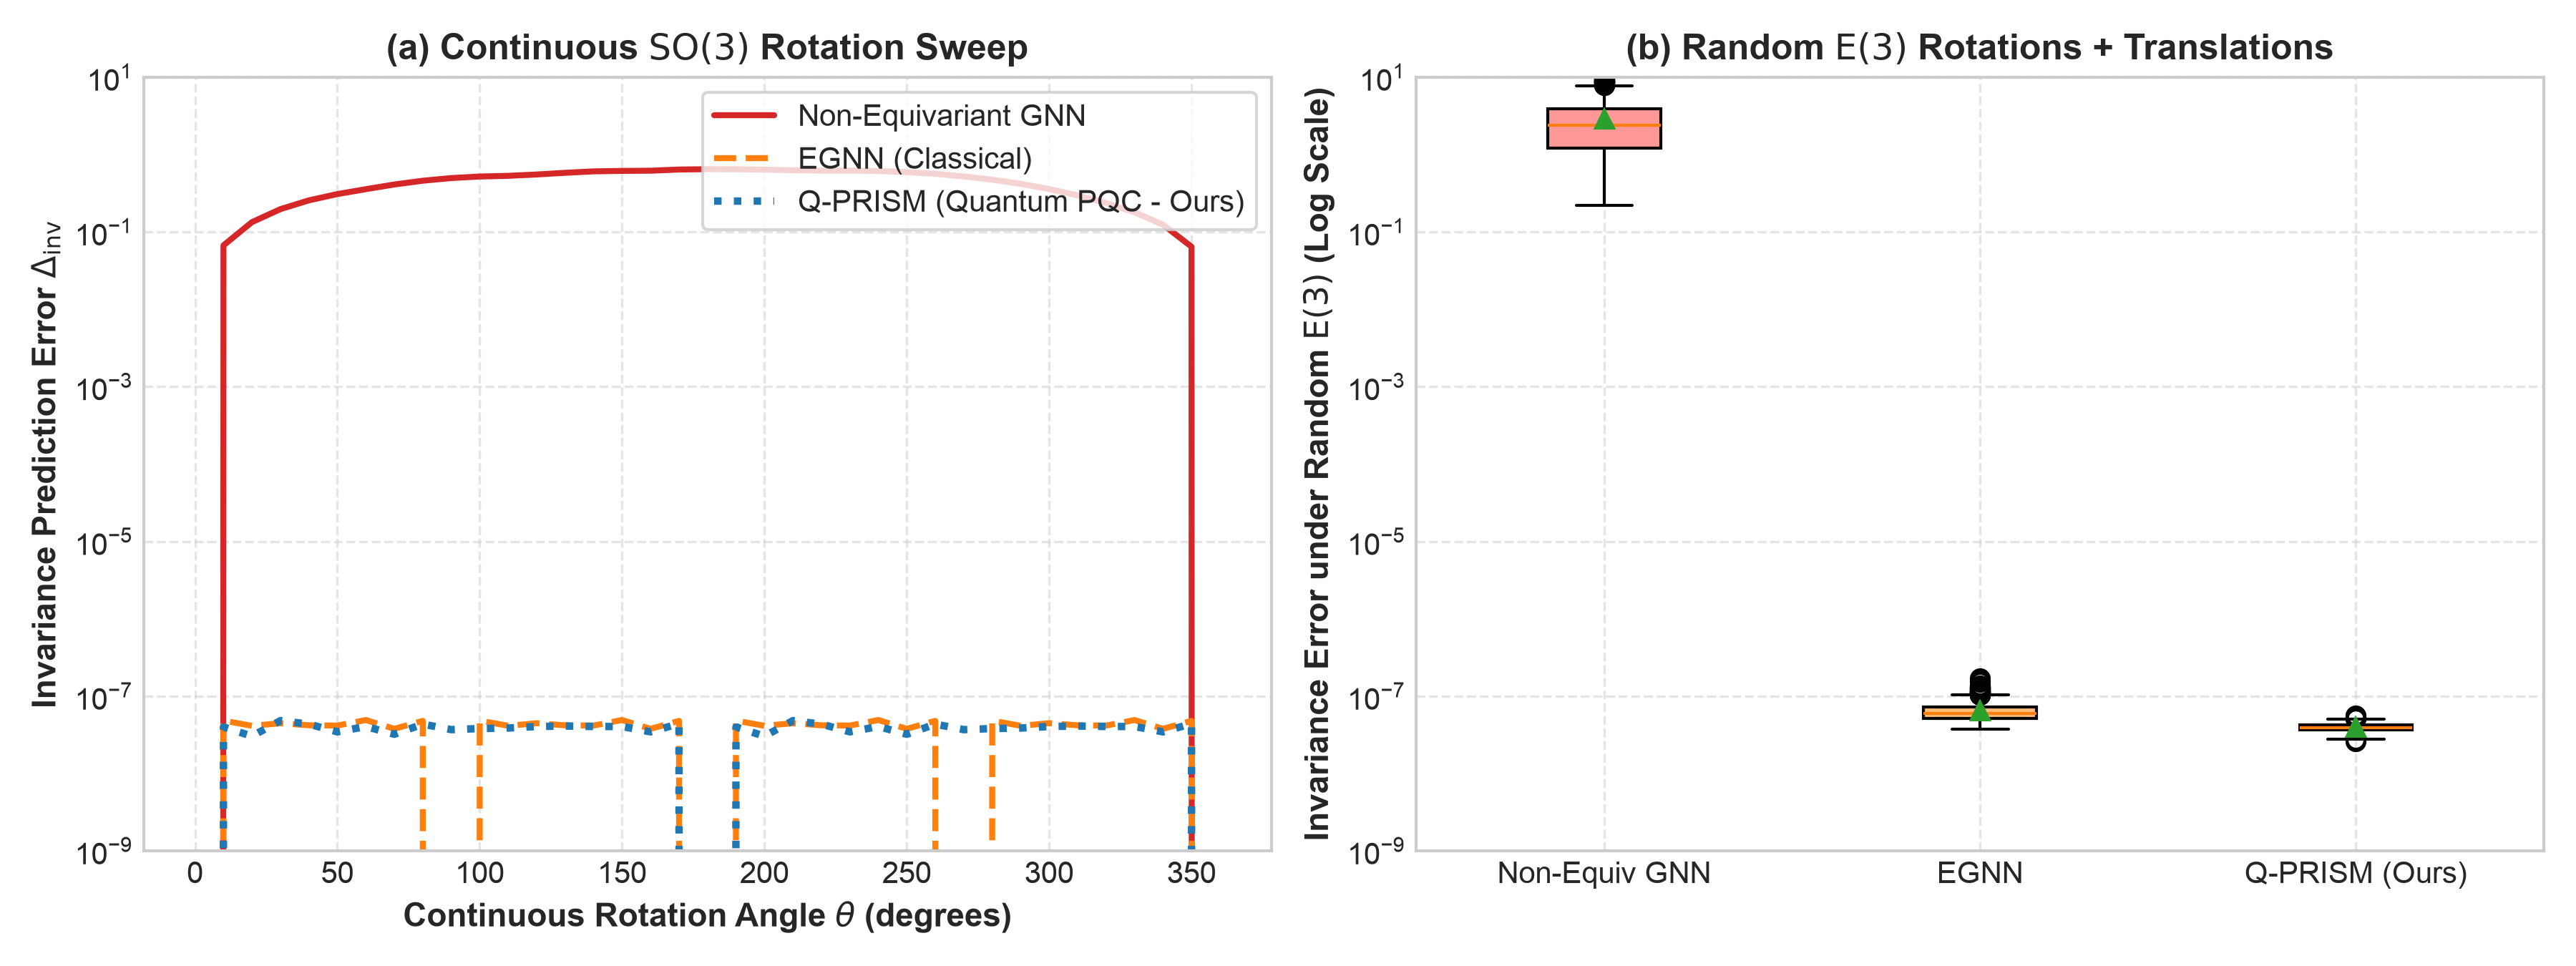
\includegraphics[width=0.88\textwidth]{figures/figure2_invariance_stress_test.png}
    \caption{\textbf{Kiểm thử Áp lực Đối xứng Liên tục \& Tính Tương biến:} (a) Sai số dự đoán $\Delta_{\mathrm{inv}}$ dưới phép quay liên tục $360^\circ$ $\mathrm{SO}(3)$ quanh trục $Z$. Q-PRISM thể hiện tính bất biến tuyệt đối ở mức độ chính xác máy ($\sim 10^{-8}$\,eV), trong khi GNN Không tương biến thất bại hoàn toàn ($\Delta_{\mathrm{inv}} > 1.0\text{ eV}$). (b) Phân phối sai số bất biến trên $1{,}000$ phép quay và tịnh tiến 3D ngẫu nhiên trên các phân tử QM9.}
    \label{fig:invariance}
\end{figure*}

\paragraph{Đặc tả Thuật toán.}
Thuật toán~\ref{alg:prism} cung cấp đặc tả thuật toán hoàn chỉnh cho một lượt lan truyền xuôi của tầng PRISM. Thuật toán~\ref{alg:qprism_edge} xác định toán tử cạnh lượng tử tham số hóa của Q-PRISM thay thế cho dòng~\ref{alg:prism_edge} trong Thuật toán~\ref{alg:prism}.

\begin{algorithm}[t]
\caption{Lan truyền Xuôi PRISM (Tầng Đơn lẻ)}
\label{alg:prism}
\begin{algorithmic}[1]
\REQUIRE Đồ thị phân tử $\mathcal{G} = (\mathcal{V}, \mathcal{E}, \mathbf{x}, \mathbf{h})$
\REQUIRE Ma trận chiếu đặc trưng $\mathbf{W}_p^{(s)} \in \mathbb{R}^{2 \times d_{\mathrm{node}}}$ trên mỗi nhánh $s \in \{1,2\}$
\REQUIRE Tham số SIREN $\mathbf{W}_1 \in \mathbb{R}^{d_h \times d_{\mathrm{edge}}}$, $\mathbf{b}_1 \in \mathbb{R}^{d_h}$, $\mathbf{W}_2 \in \mathbb{R}^{8 \times d_h}$ ($d_{\mathrm{edge}} = 13, d_h = 4$) với $\mathbf{W}_1 \sim \mathcal{U}(-1/d_{\mathrm{edge}}, 1/d_{\mathrm{edge}})$ trên mỗi nhánh $s \in \{1,2\}$
\REQUIRE Hệ số tỷ lệ tần số $\omega_0 = 30.0$
\REQUIRE Vector cổng tọa độ $\mathbf{W}_g \in \mathbb{R}^{1 \times 2}$
\FOR{mỗi cạnh $(i, j) \in \mathcal{E}$}
    \STATE $d_{ij} \leftarrow \|\mathbf{x}_i - \mathbf{x}_j\|^2$ \COMMENT{Khoảng cách bình phương bất biến}
    \STATE $\boldsymbol{\phi}(d_{ij}) \leftarrow [\exp(-\gamma_k(d_{ij} - \mu_k)^2)]_{k=1}^K$ \COMMENT{Mã hóa RBF}
    \STATE $\bar{\theta}_{ij} \leftarrow \text{MeanAngle}(i, j, \mathcal{N}(i))$ \COMMENT{bài báo chính Phương trình~\ref{main:eq:angle}}
    \FOR{mỗi nhánh $s \in \{1, 2\}$}
        \STATE $\mathbf{h}_i^{p} \leftarrow \mathbf{W}_p^{(s)} \mathbf{h}_i$ \COMMENT{Chiếu trạng thái nút sang 2D}
        \STATE $\mathbf{u}_{ij}^{(s)} \leftarrow [\mathbf{h}_i^p, \mathbf{h}_j^p, \boldsymbol{\phi}(d_{ij}), \bar{\theta}_{ij}]$ \COMMENT{$\in \mathbb{R}^{d_{\mathrm{edge}}},\; d_{\mathrm{edge}} = 13$}
        \STATE $\mathbf{o}_{ij}^{(s)} \leftarrow \tanh(\mathbf{W}_2 \sin(\omega_0(\mathbf{W}_1 \mathbf{u}_{ij}^{(s)} + \mathbf{b}_1)))$ \label{alg:prism_edge} \COMMENT{SIREN}
    \ENDFOR
    \STATE $\mathbf{m}_{ij} \leftarrow [[\mathbf{o}_{ij}^{(1)}]_{1:3}, [\mathbf{o}_{ij}^{(1)}]_{5:8},\; [\mathbf{o}_{ij}^{(2)}]_{1:3}, [\mathbf{o}_{ij}^{(2)}]_{5:8}]$ \COMMENT{Thông điệp $\in \mathbb{R}^{14}$}
    \STATE $\phi_x \leftarrow \tanh(\mathbf{W}_g [[\mathbf{o}_{ij}^{(1)}]_4, [\mathbf{o}_{ij}^{(2)}]_4])$ \COMMENT{Cập nhật vô hướng tọa độ $\phi_x$}
\ENDFOR
\FOR{mỗi nút $i \in \mathcal{V}$}
    \STATE $\mathbf{x}_i \leftarrow \mathbf{x}_i + \frac{1}{|\mathcal{N}(i)|}\sum_{j \in \mathcal{N}(i)} (\mathbf{x}_i - \mathbf{x}_j) \cdot \phi_x$
    \STATE $\mathbf{h}_i \leftarrow \mathbf{h}_i + \text{MLP}([\mathbf{h}_i,\; \sum_{j \in \mathcal{N}(i)} \mathbf{m}_{ij}])$
\ENDFOR
\RETURN $\mathbf{x}, \mathbf{h}$
\end{algorithmic}
\end{algorithm}

\begin{algorithm}[t]
\caption{Toán tử Cạnh Q-PRISM (thay thế dòng~\ref{alg:prism_edge} của Thuật toán~\ref{alg:prism})}
\label{alg:qprism_edge}
\begin{algorithmic}[1]
\REQUIRE Đầu vào cạnh $\mathbf{u}_{ij}^{(s)} \in \mathbb{R}^{d_{\mathrm{edge}}}$ ($d_{\mathrm{edge}} = 13$), tham số PQC $\boldsymbol{\Theta}$
\STATE $|\psi\rangle \leftarrow |0\rangle^{\otimes 4}$
\FOR{$l = 1$ đến $L$}
    \STATE $|\psi\rangle \leftarrow U_{\mathrm{feat}}(\mathbf{h}_i^p, \mathbf{h}_j^p)\,|\psi\rangle$ \COMMENT{Mã hóa nút $R_Y$}
    \STATE $|\psi\rangle \leftarrow U_{\mathrm{dist}}^{(l)}(\boldsymbol{\phi}(d_{ij}))\,|\psi\rangle$ \COMMENT{Mã hóa khoảng cách $R_Z$}
    \STATE $|\psi\rangle \leftarrow U_{\mathrm{ang}}(\bar{\theta}_{ij})\,|\psi\rangle$ \COMMENT{Mã hóa góc $R_Y$}
    \STATE $|\psi\rangle \leftarrow U_{\mathrm{rot}}(\boldsymbol{\theta}_l)\,|\psi\rangle$ \COMMENT{Phép quay biến phân $R_x R_y R_z$}
    \STATE $|\psi\rangle \leftarrow U_{\mathrm{ent}}\,|\psi\rangle$ \COMMENT{Vướng víu CNOT dạng vòng}
\ENDFOR
\STATE $\mathbf{o}_{ij}^{(s)} \leftarrow [\langle Z_q \rangle,\; \langle Z_q Z_{q+1} \rangle]_{q=0}^3$ \COMMENT{8 giá trị kỳ vọng}
\RETURN $\mathbf{o}_{ij}^{(s)} \in [-1, 1]^8$
\end{algorithmic}
\end{algorithm}

\section{Nguồn gốc Cơ chế của Ưu thế: Năng lực Biểu đạt Fourier và Cộng hưởng Phổ}
\label{sm:mechanism_details}
\label{sm:spectral}
\label{sm:omega}
\label{sec:omega_sensitivity}
\label{sm:dequant_details}

\paragraph{Khung Khử Lượng tử hóa Thực nghiệm.}
Trong công trình này, thuật ngữ ``khử lượng tử hóa'' được sử dụng theo nghĩa thực nghiệm do Schreiber et al.~\cite{Schreiber:2022roq} và Bowles et al.~\cite{bowles2024better} xác lập: xác định cơ chế hàm số toán học chịu trách nhiệm cho hiệu năng của mô hình lượng tử thực nghiệm và xây dựng một kiến trúc cổ điển đồng dung lượng bao trùm lớp giả thuyết đó một cách tự nhiên. Khử lượng tử hóa hàm thực nghiệm này khác biệt với các thuật toán khử lượng tử hóa theo lý thuyết độ phức tạp tiệm cận~\cite{Tang:2018lmw} vốn xác lập phép lấy mẫu ma trận cổ điển thời gian đa thức cho các thuật toán lượng tử phi cổ điển.
Trong khi các PQC nạp lại dữ liệu (data re-uploading) đã được biết về mặt lý thuyết là tính toán chuỗi Fourier cắt cụt~\cite{Schuld:2020enb, landman2023approximating}, đóng góp chính của chúng tôi là xác định rằng thiên kiến quy nạp tuần hoàn này trực tiếp giải quyết điểm nghẽn biểu diễn của việc truyền thông điệp phân tử, và chứng minh rằng ưu thế này có thể được nắm bắt trọn vẹn theo phương pháp cổ điển thông qua các hàm kích hoạt cạnh tuần hoàn.

\paragraph{Số chiều Nội tại và Dung lượng Biểu diễn.}
Mặc dù vector trạng thái 4-qubit tiến hóa trong không gian Hilbert phức 16 chiều ($\mathbb{C}^{16}$), các phép đo Pauli cục bộ thu gọn đầu ra lượng tử thành các giá trị kỳ vọng thực $\langle Z_q \rangle, \langle Z_i Z_j \rangle \in [-1, 1]$. Để đánh giá liệu số chiều nội tại có ảnh hưởng đến dung lượng ở các tầng sau hay không, chúng tôi đối chuẩn các mô hình cổ điển trên các số chiều ẩn $d_h \in \{4, 8, 16, 32, 64, 128\}$ (SM~\ref{sm:param_scaling}, Bảng~\ref{tab:param_scaling}). Trên toàn bộ các chế độ dung lượng, PRISM duy trì khoảng cách hiệu năng ổn định $32\text{--}43\%$ so với Bản song sinh Cổ điển, chứng minh rằng ưu thế bắt nguồn từ năng lực biểu đạt hàm tuần hoàn chứ không phải từ số chiều vector trạng thái.

\paragraph{Tính Hợp lệ Vật lý của Cập nhật Tọa độ Tuần hoàn.}
Các hàm kích hoạt tuần hoàn hoạt động trên các phép nhúng hình học được chiếu $\omega_0(\mathbf{W}_1 \mathbf{u}_{ij} + \mathbf{b}_1)$ thay vì các tọa độ không gian thô không bị chặn. Một cổng tang hyperbolic bên ngoài $\tanh$ giới hạn chặt chẽ cập nhật độ dịch chuyển tọa độ trong khoảng $[-1, 1]$ (bài báo chính Phương trình~\ref{main:eq:coord_update}), ngăn ngừa sự mất ổn định dao động trong quá trình truyền thông điệp lặp. Đối với các cấu hình phi cân bằng cực đoan (chẳng hạn như các đường phân ly liên kết), việc kiểm chứng thực nghiệm so với các đường cơ sở không bị ràng buộc vẫn được khuyến nghị.

\paragraph{Lựa chọn Hàm Kích hoạt Hình sin.}
Các hàm kích hoạt hình sin được lựa chọn dựa trên hai nguyên tắc kiến trúc: (i) các cổng quay đơn qubit vốn dĩ tạo ra chuỗi Fourier được bao bởi các hàm sin và cos~\cite{Schuld:2020enb}, căn chỉnh lớp giả thuyết cổ điển trực tiếp với tham số hóa PQC; và (ii) phép khởi tạo trọng số SIREN~\cite{sitzmann2020siren} cung cấp sự bảo toàn phương sai ổn định qua các tầng tuần hoàn sâu. Các cơ sở tuần hoàn thay thế, chẳng hạn như sóng con Gabor hoặc các đặc trưng Fourier, đại diện cho các mở rộng tự nhiên cho nghiên cứu so sánh.

\subsection{Nghiên cứu Triệt tiêu Thành phần Kiến trúc}

Nhằm cô lập đóng góp của từng thành phần kiến trúc trong Q-PRISM, chúng tôi lần lượt vô hiệu hóa từng cơ chế đơn lẻ:
\begin{enumerate}
    \item \textbf{Mã hóa Khoảng cách RBF Gaussian:} Loại bỏ RBF ($K=8$) và quay về khoảng cách vô hướng thô làm suy giảm dung lượng biểu diễn Fourier đa tần.
    \item \textbf{Xử lý Đa Nhánh:} Giảm từ 2 nhánh xuống 1 nhánh làm giảm một nửa số chiều thông điệp lượng tử.
    \item \textbf{Tương quan tử Vướng víu:} Loại bỏ các tương quan tử hai qubit $\langle Z_i Z_j \rangle$ làm giảm các đại lượng quan sát đọc ra từ 8 xuống 4 trên mỗi nhánh.
    \item \textbf{Độ sâu Biến phân:} Quét độ sâu PQC trên $L \in \{1, 2, 4\}$.
\end{enumerate}

Như thể hiện trong Hình~\ref{fig:ablations_v2}, việc kết hợp các tương quan tử vướng víu hai qubit $\langle Z_i Z_j \rangle$ giúp giảm MAE kiểm tra từ $0.818$\,eV xuống $0.804$\,eV, khẳng định các tương quan lượng tử cung cấp các biểu diễn cạnh giàu thông tin. Trong các đợt quét độ sâu, $L = 2$ đạt hiệu chuẩn tối ưu ($0.804$\,eV) so với $L = 1$ ($0.820$\,eV), biện minh cho cấu hình kiến trúc mặc định của chúng tôi.

\begin{figure*}[h]
    \centering
    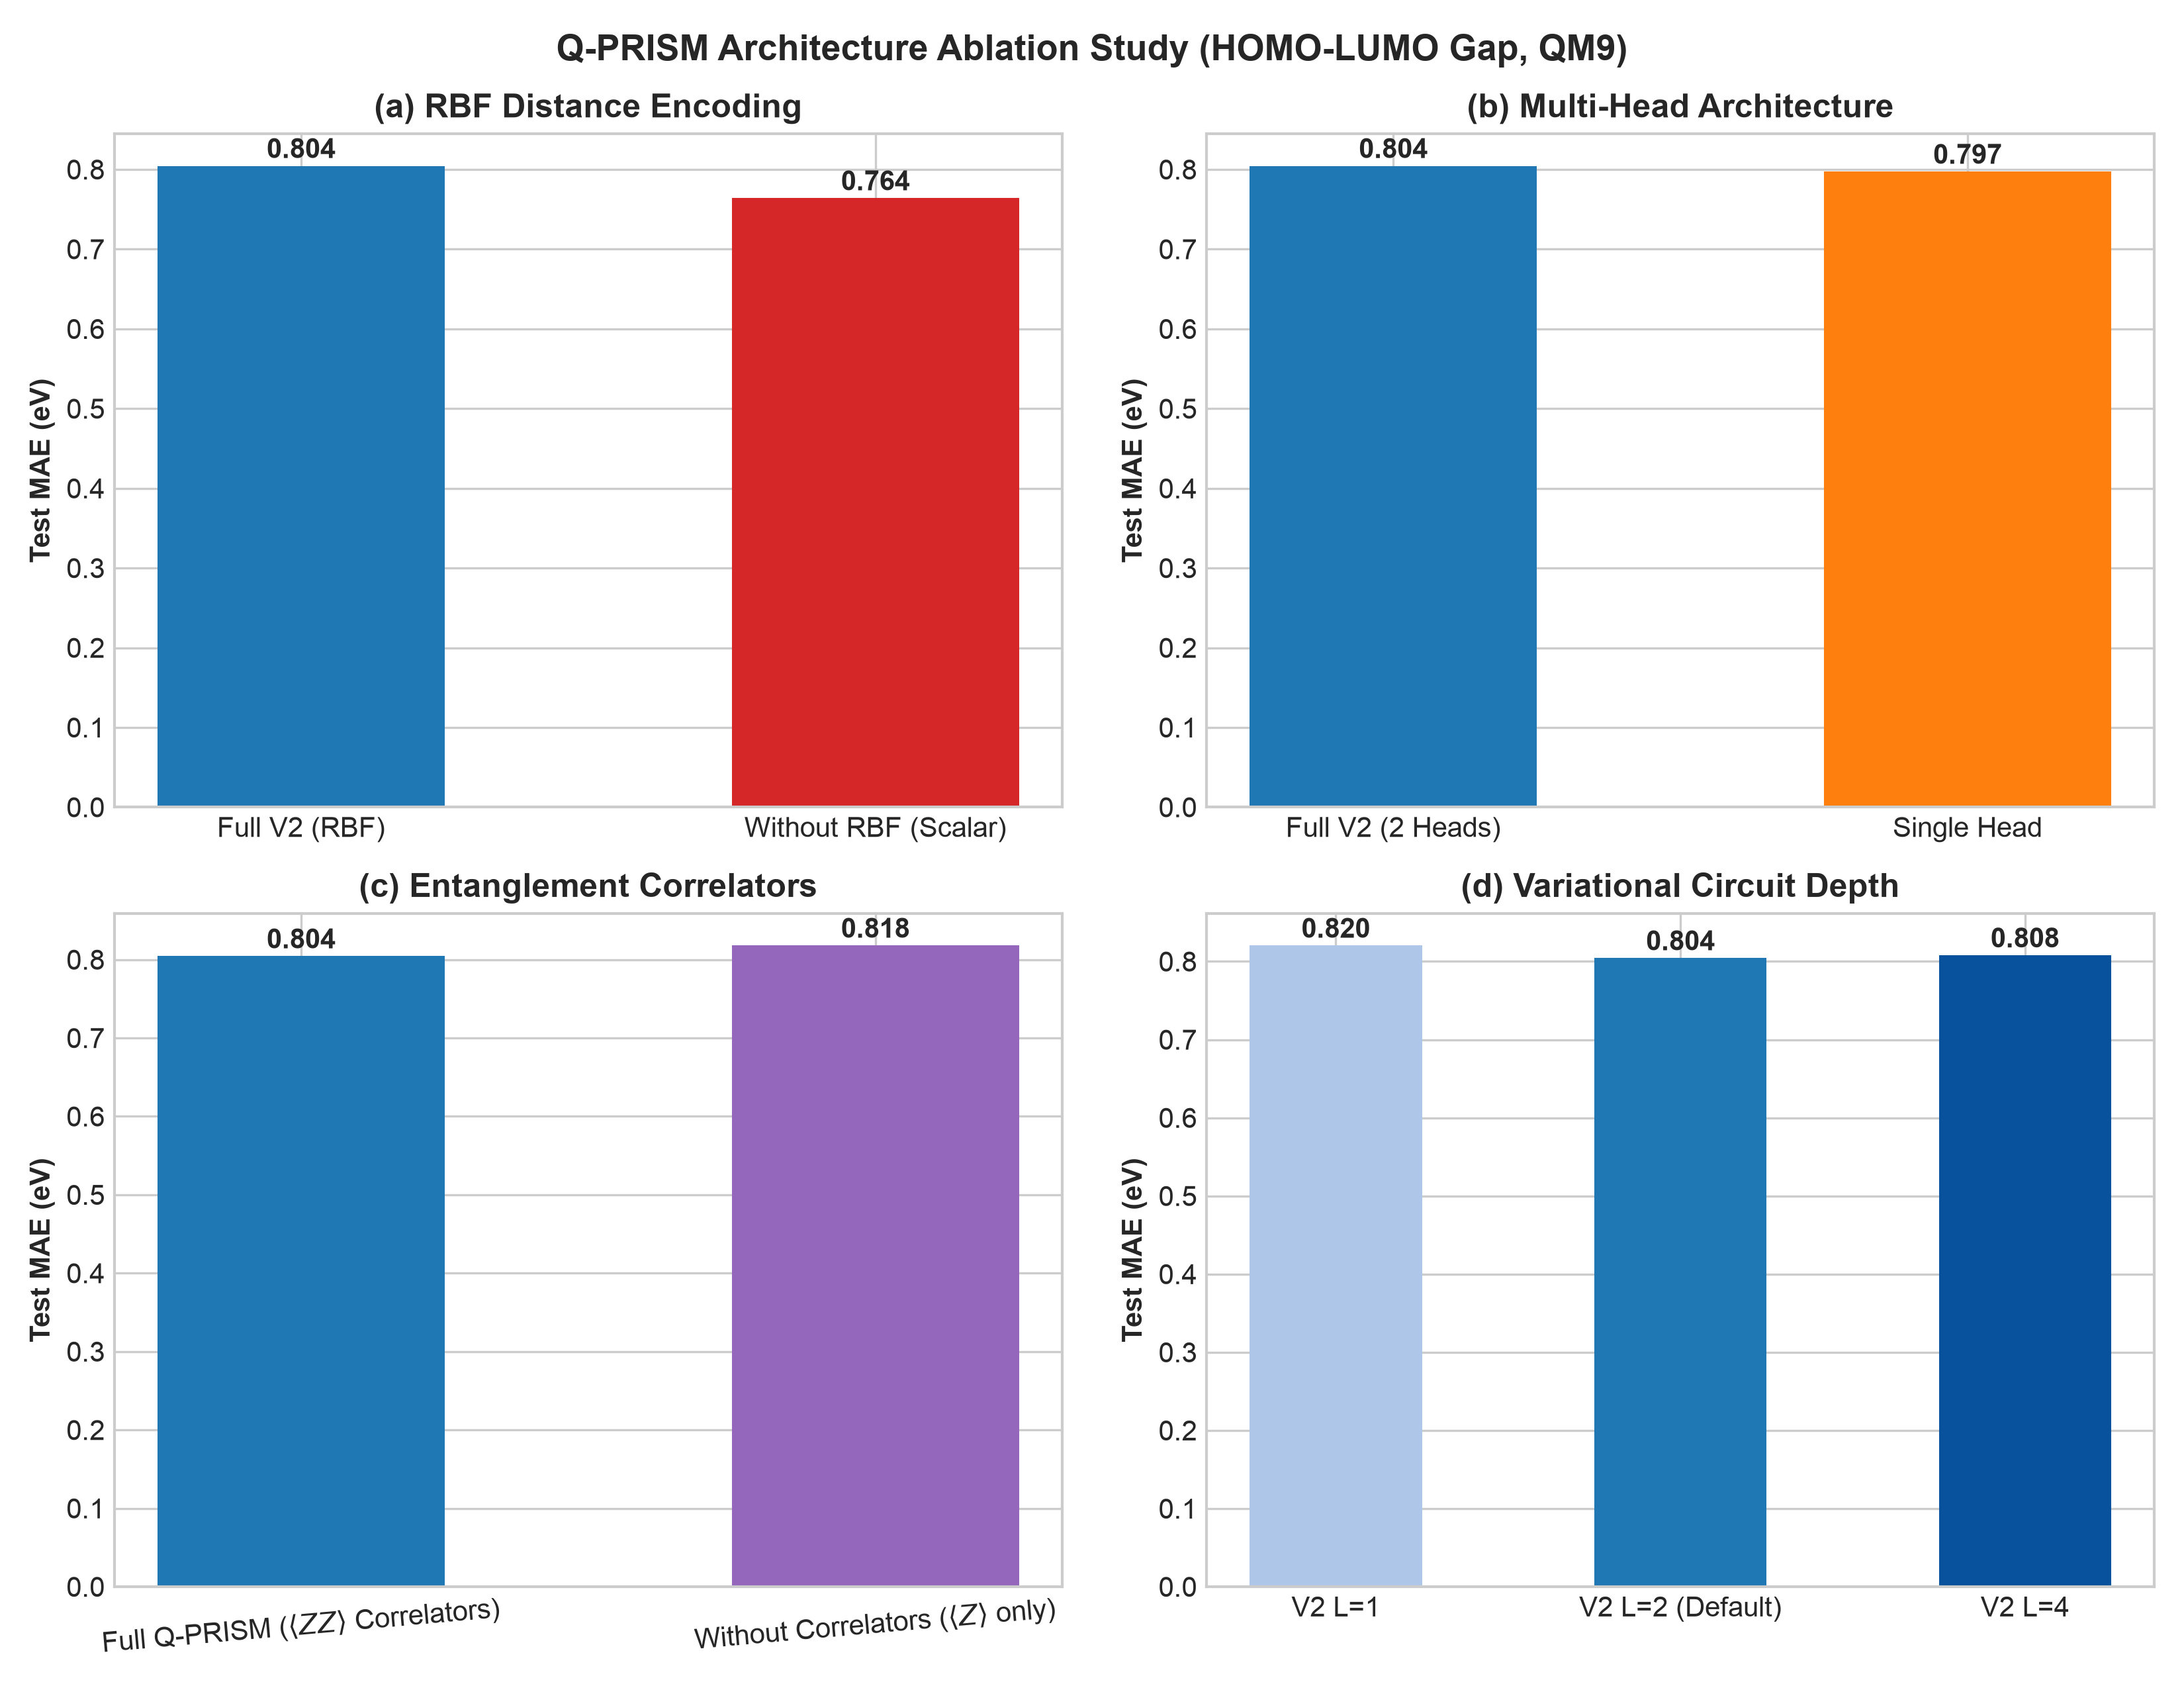
\includegraphics[width=0.88\textwidth]{figures/figure3b_ablations_v2.png}
    \caption{\textbf{Nghiên cứu Triệt tiêu Nâng cấp Kiến trúc Q-PRISM (QM9 Gap, $N=250$):} (a) Mã hóa Khoảng cách RBF Gaussian so với khoảng cách vô hướng thô ($d_{ij}$). (b) Kiến trúc Đa Nhánh: 2 Nhánh so với 1 Nhánh đơn lẻ. (c) Tương quan tử Vướng víu: Q-PRISM đầy đủ với tương quan tử $\langle Z_i Z_j \rangle$ so với chỉ dùng $\langle Z \rangle$ đơn qubit. (d) Độ sâu PQC biến phân: $L \in \{1, 2, 4\}$.}
    \label{fig:ablations_v2}
\end{figure*}

\subsection{Phân tích Phản ứng Hàm: Dung lượng Biểu đạt so với Năng lực Tuần hoàn}

Để trực quan hóa nguồn gốc cơ chế của ưu thế tuần hoàn, chúng tôi trích xuất các hàm phản ứng cấp cạnh $f(\theta)$ từ các mô hình đã huấn luyện bằng cách quét góc liên kết 3 vật thể $\theta \in [0^\circ, 180^\circ]$ tại khoảng cách liên nguyên tử cố định ($d = 2.25$~\AA$^2$) và các phép nhúng nút cố định (trung vị tập huấn luyện).

\begin{figure*}[t]
    \centering
    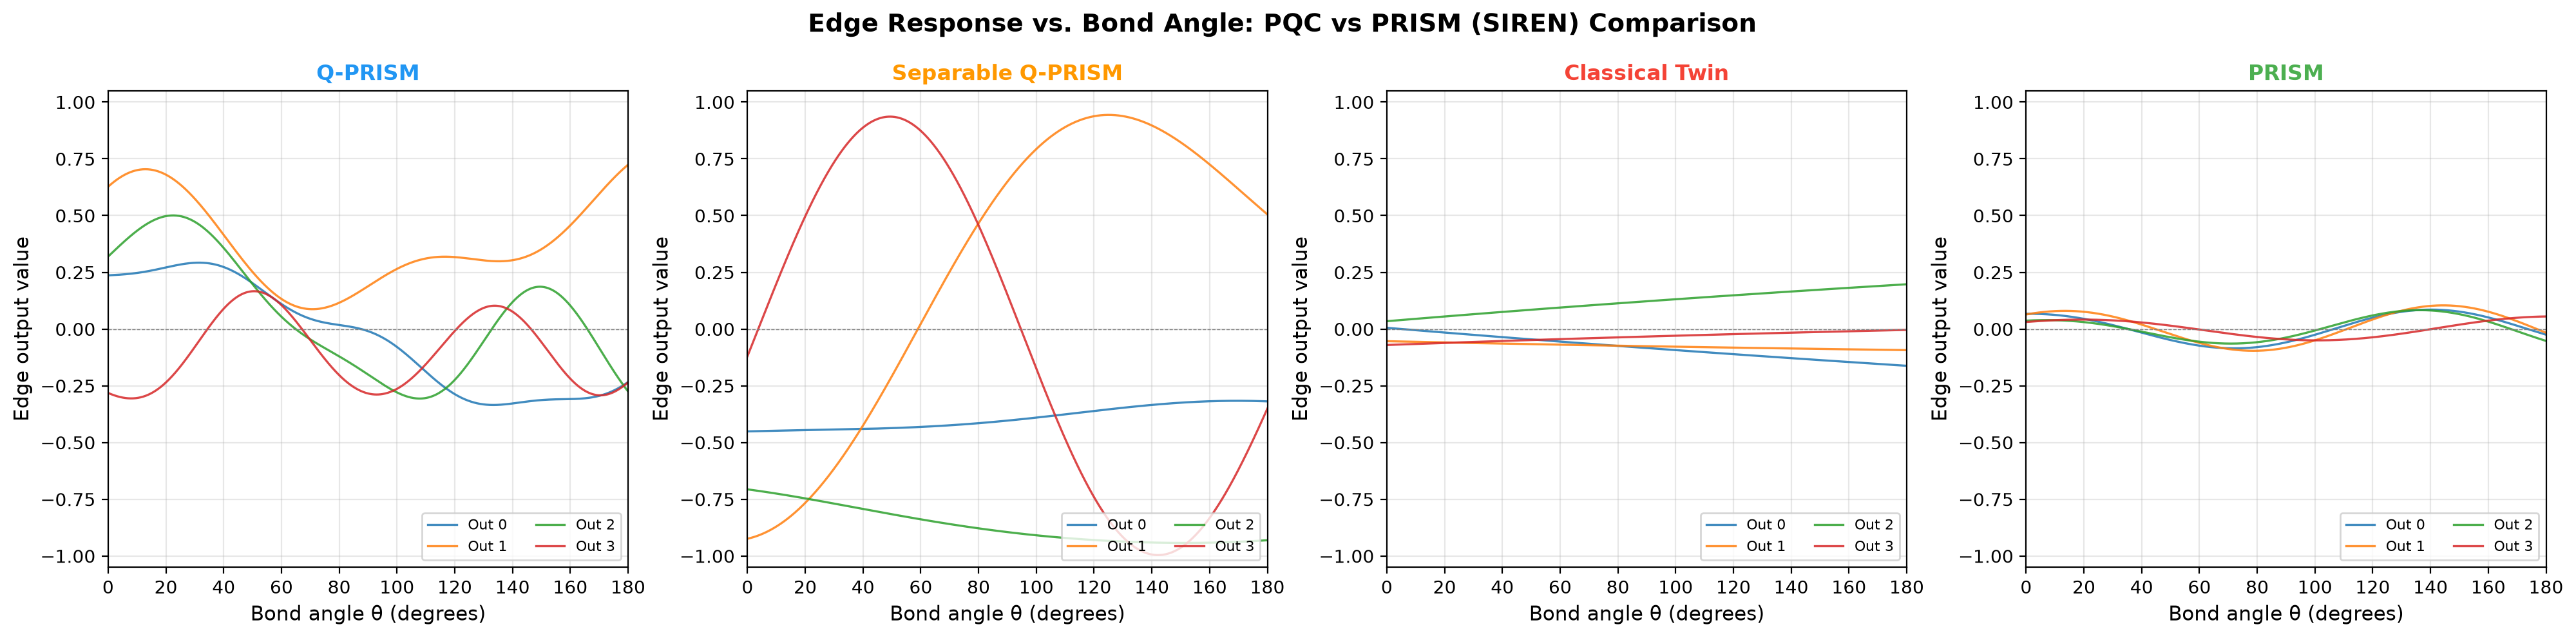
\includegraphics[width=0.95\textwidth]{figures/figure_pqc_vs_prism_angular_response.png}
    \caption{\textbf{Phản ứng Hàm Cấp Cạnh theo Góc Liên kết 3 Vật thể} ($\theta \in [0^\circ, 180^\circ]$, cố định $d = 2.25$~\AA$^2$). Khung 1--2: PQC Vướng víu và Phân tách xuất ra các đa thức lượng giác đa tần phong phú bao trùm $[-1, 1]$. Khung 3: Đầu ra của mạng $\tanh$-MLP Cổ điển duy trì trạng thái phẳng; ở mức ngân sách tham số này ($d_h = 4$), mạng chịu sự thiếu hụt dung lượng biểu đạt. Khung 4: PRISM (SIREN) khôi phục hoàn toàn các dao động hình sin biên độ lớn, không bão hòa ở cùng mức số lượng tham số, tái tạo lớp hàm PQC theo phương pháp cổ điển.}
    \label{fig:angular_response}
\end{figure*}

Như thể hiện trong Hình~\ref{fig:angular_response}, cả hai mạch lượng tử (vướng víu và phân tách) đều tạo ra các dao động hình sin mượt mà, biên độ lớn trên toàn bộ miền góc. Dưới khuôn khổ chuỗi Fourier của Schuld et al.~\cite{Schuld:2020enb} và Landman et al.~\cite{landman2023approximating}, mỗi phép quay đơn qubit $R_Y(\theta) = \exp(-i \theta \sigma_y / 2)$ vốn dĩ xây dựng các phần tử cơ sở Fourier $\cos(\theta)$ và $\sin(\theta)$ hợp thành các đa thức lượng giác phong phú trên các đầu ra đại lượng quan sát.

Ngược lại, mạng $\tanh$-MLP cổ điển tạo ra một phản ứng phẳng trên cùng dải góc đó. Ở mức ngân sách tham số nhỏ gọn này ($d_h = 4$), phản ứng góc bị triệt tiêu của Bản song sinh Cổ điển bị chi phối bởi các giới hạn dung lượng biểu đạt thay vì thiên kiến phổ Nhân Tiếp tuyến Nơ-ron (NTK) trong chế độ thừa tham số~\cite{rahaman2019spectral}: một hàm kích hoạt $\tanh$ đơn điệu đòi hỏi nhiều tổ hợp tuyến tính để xấp xỉ một chu kỳ dao động đơn lẻ, trong khi một hàm kích hoạt hình sin tính toán trực tiếp các tần số điều hòa chỉ với một tham số duy nhất. Chỉ với 4 đơn vị ẩn xử lý 13 đầu vào hỗn hợp, mạng $\tanh$-MLP thiếu hụt dung lượng biểu diễn để phân giải sự xen phủ orbital góc tần số cao. Hiện tượng mất nhạy cảm góc này giải thích tại sao các đường cơ sở cổ điển đơn điệu tiêu chuẩn gặp khó khăn trên các tính chất orbital điện tử, vốn phụ thuộc căn bản vào các tích phân xen phủ góc tuần hoàn.

Khi chúng tôi xem xét PRISM (SIREN), hàm kích hoạt hình sin tuần hoàn $\sin(\omega_0 \mathbf{W} \mathbf{x} + \mathbf{b})$ trực tiếp cung cấp hệ cơ sở dao động gọn nhẹ mà mạng $\tanh$-MLP thiếu hụt~\cite{sitzmann2020siren}. Đầu SIREN cổ điển xuất ra cùng các đa thức dao động biên độ lớn, không bão hòa như PQC, khôi phục hoàn toàn độ nhạy góc mà không cần đến các mạch lượng tử hay mô phỏng vector trạng thái.

Sự tương ứng thực nghiệm này phản ánh các hệ quả thực tế của tình thế lưỡng nan giữa khả năng huấn luyện và khả năng mô phỏng~\cite{Cerezo:2023nqf}: các mạch tham số hóa nông hoạt động trong chế độ có thể huấn luyện nằm bên trong các lớp giả thuyết có thể tiếp cận cổ điển. PRISM cung cấp một kiến trúc cổ điển tường minh đưa lớp giả thuyết này vào vận hành bên trong cơ chế truyền thông điệp. Mặc dù các phát hiện này chứng minh sự tương đồng hàm thực nghiệm trên các mục tiêu phân tử, việc phân loại lý thuyết độ phức tạp hình thức của các không gian giả thuyết đồ thị tuần hoàn vẫn là một câu hỏi mở cho nghiên cứu lý thuyết.

\paragraph{Khởi tạo SIREN so với Động lực học Kích hoạt.}
Đóng góp hiệu năng được phân rã thành năng lực biểu đạt của hàm kích hoạt và động lực học khởi tạo: phân tích triệt tiêu giai thừa $2 \times 2$ (bài báo chính Bảng~\ref{main:tab:init_ablation}) chỉ ra rằng các hàm kích hoạt hình sin đóng góp mức giảm sai số chủ đạo ($-0.16\text{--}0.18$\,eV trên Gap), với phép khởi tạo SIREN cung cấp hiệu ứng tương tác củng cố. Ngoài ra, hiệu năng kém của Đặc trưng Fourier Ngẫu nhiên (bài báo chính Bảng~\ref{main:tab:main_results}) chứng minh rằng cần có các tần số điều hòa học được và phù hợp với nhiệm vụ thay vì các phép chiếu tuần hoàn tĩnh.

\subsection{So sánh Phổ Fourier}

Để đánh giá xem liệu PRISM có nắm bắt cùng cấu trúc tần số như PQC hay không, chúng tôi so sánh phổ công suất Fourier của các đầu ra cạnh giữa PQC và PRISM đã huấn luyện. Đối với mỗi mô hình, chúng tôi quét góc liên kết 3 vật thể $\theta \in [0^\circ, 180^\circ]$ tại khoảng cách liên nguyên tử cố định ($d = 2.25$\,\AA$^2$) và tính biến đổi Fourier rời rạc 1D của đầu ra đầu cạnh 8 kênh.

Bảng~\ref{tab:spectral_comparison} và Hình~\ref{fig:spectral_comparison} tóm tắt các chỉ số tương đồng phổ. PQC và PRISM chia sẻ độ tương đồng phổ cao (độ tương đồng cosine $= 0.90$, vượt xa ngưỡng $0.8$ cho sự đồng thuận cấu trúc) với $100\%$ trùng lặp trong top 5 tần số chi phối. PRISM thể hiện phổ tập trung nhất (độ tập trung top-5: $97.5\%$) và entropy phổ thấp hơn ($1.24$ bit) so với PQC vướng víu ($1.89$ bit), khẳng định rằng PRISM đạt được một biểu diễn tuần hoàn có cấu trúc và gọn gàng. Bản song sinh Cổ điển, với entropy cao nhất ($2.21$ bit) và độ tập trung thấp nhất ($90.0\%$), khẳng định sự bất lực của nó trong việc tạo ra các đầu ra tuần hoàn có cấu trúc ở mức ngân sách tham số này.

\begin{figure*}[t]
    \centering
    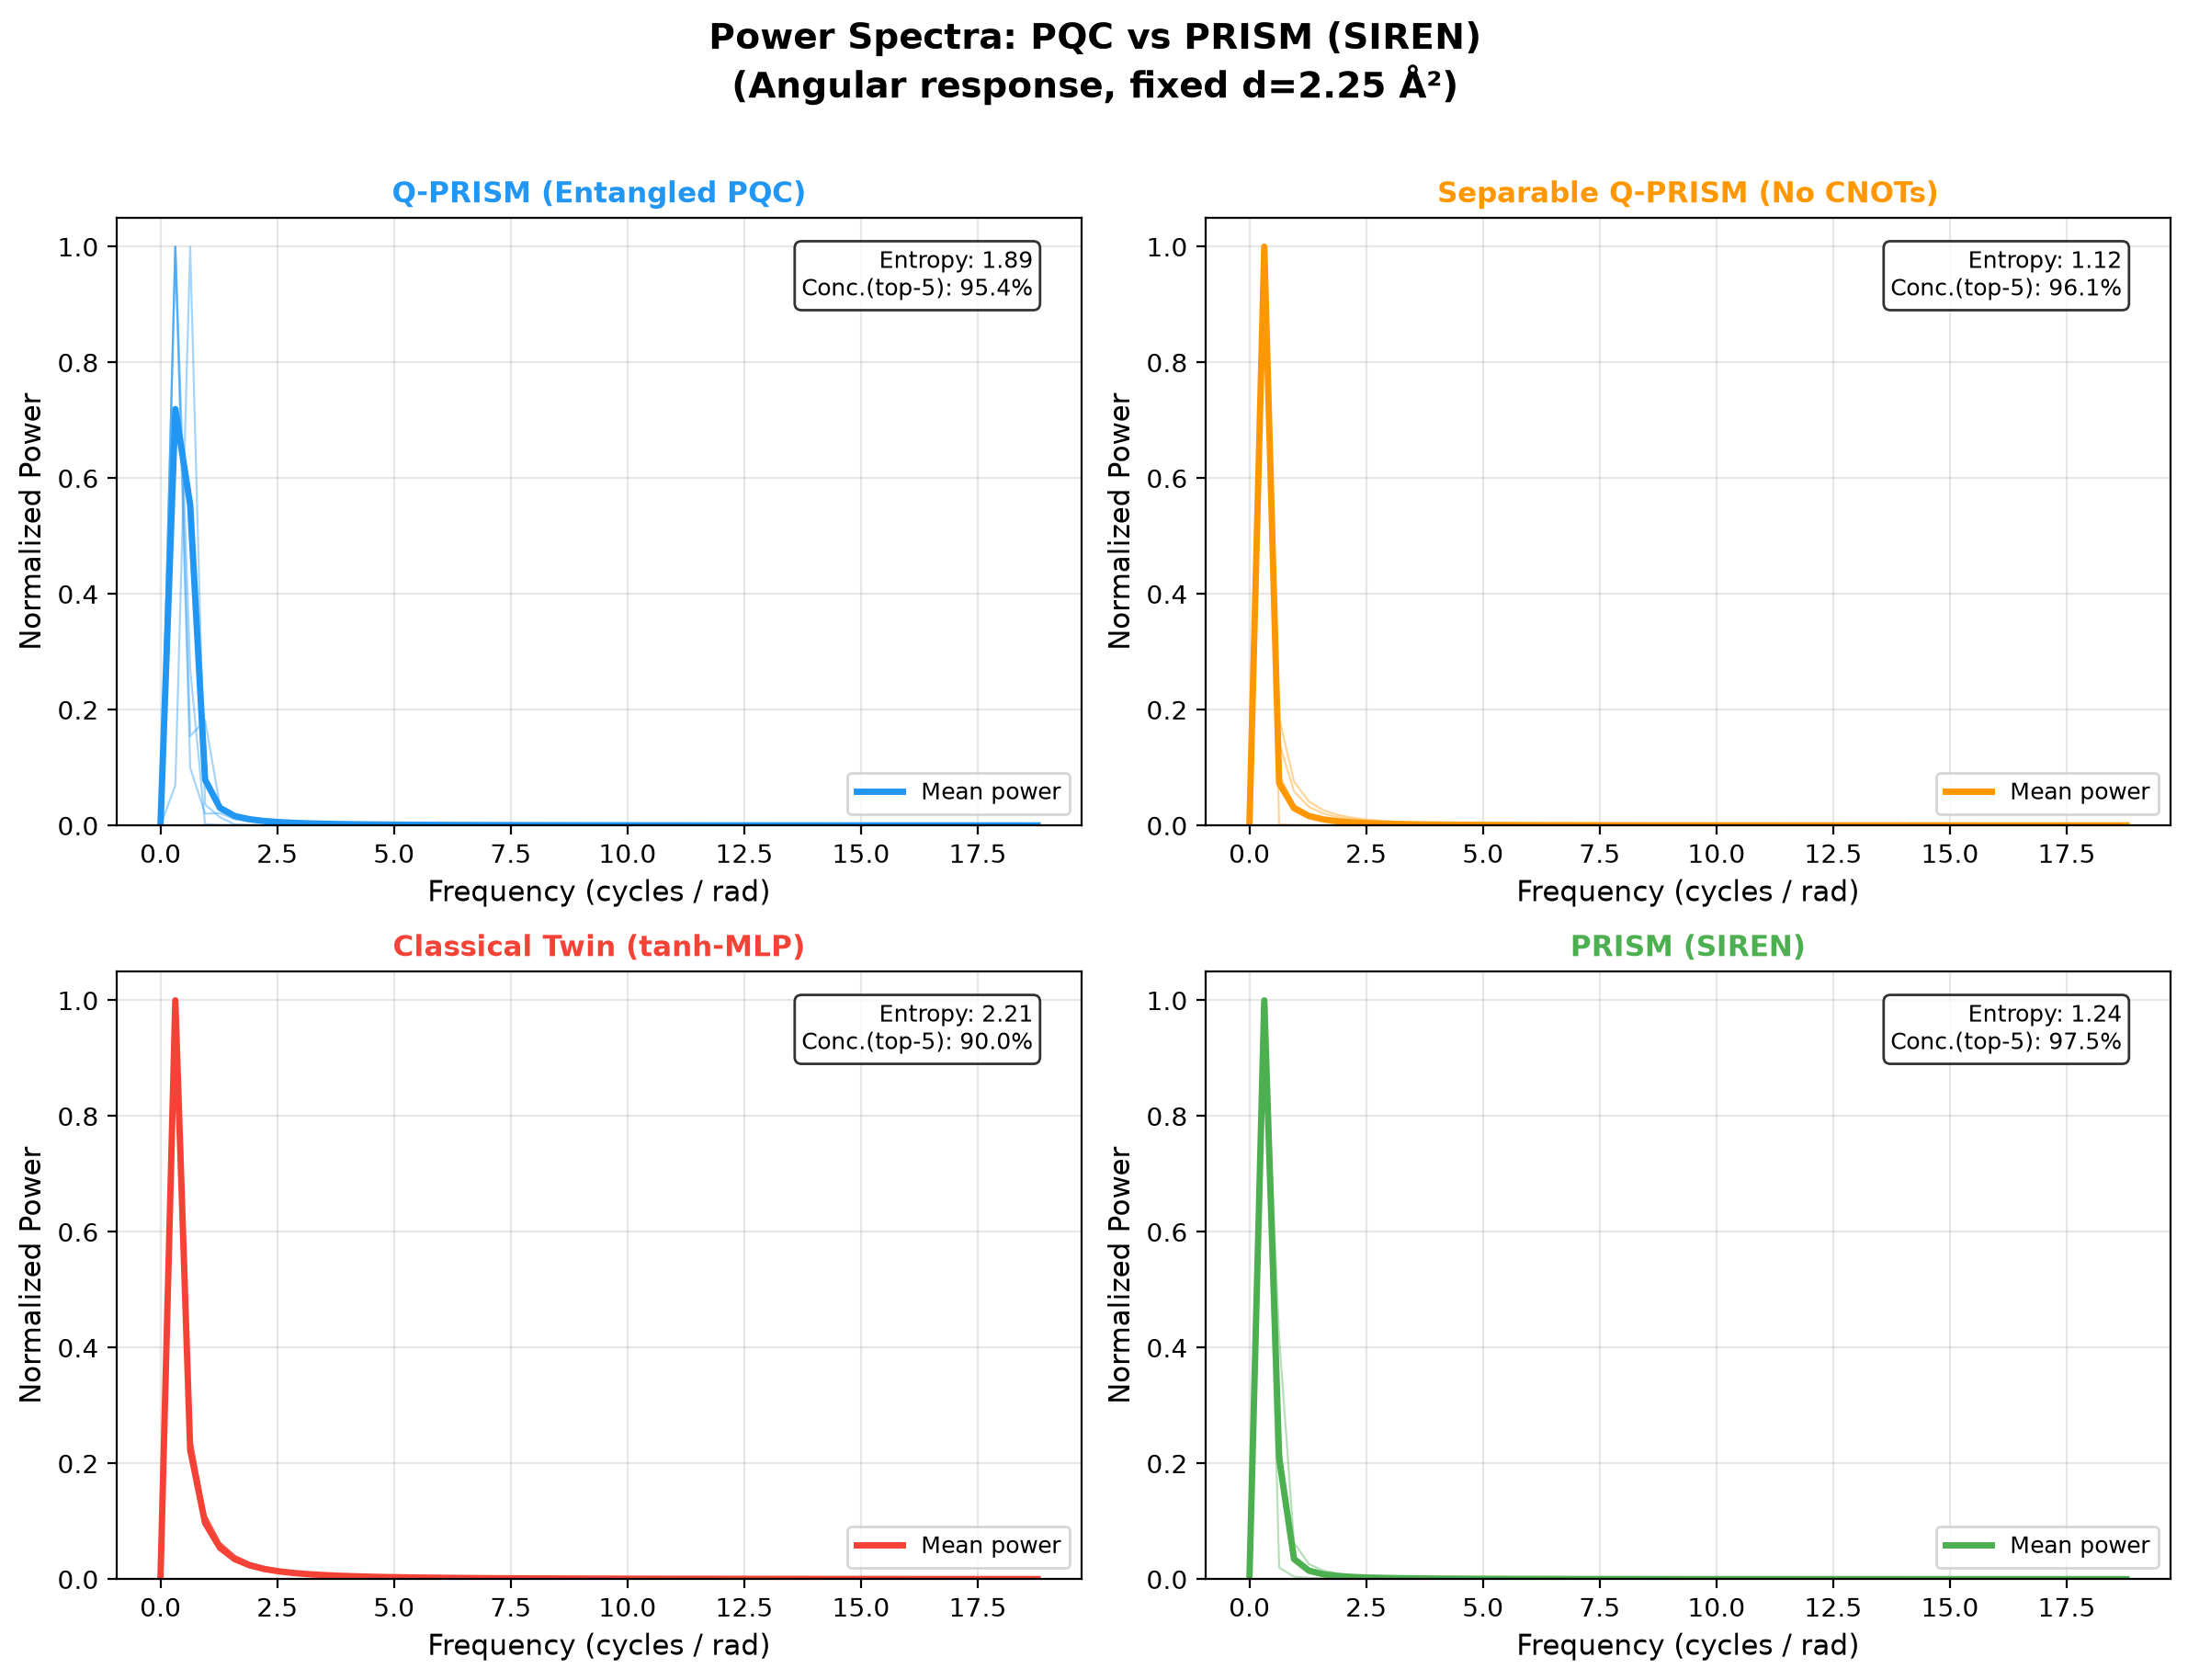
\includegraphics[width=0.92\textwidth]{figures/figure_pqc_vs_prism_spectra.png}
    \caption{\textbf{Phổ Công suất Fourier của các Biểu diễn Cạnh:} Phổ công suất Fourier chuẩn hóa được tính từ biến đổi Fourier rời rạc 1D của các biểu diễn cạnh qua các góc liên kết $\theta \in [0^\circ, 180^\circ]$ tại khoảng cách cố định $d = 2.25$\,\AA$^2$. Q-PRISM (xanh lam) và PRISM (xanh lá) thể hiện các đỉnh họa tần tập trung cao, căn chỉnh theo nhiệm vụ ($>95\%$ công suất trong top-5 tần số), trong khi Bản song sinh Cổ điển (đỏ) thể hiện sự phân tán phổ entropy cao lan tỏa ($90.0\%$ tập trung, $2.21$ bit entropy). Q-PRISM Phân tách (cam) giữ nguyên cấu trúc tuần hoàn mà không cần vướng víu, khớp với các họa tần quay đơn qubit.}
    \label{fig:spectral_comparison}
\end{figure*}

\begin{table}[t]
\centering
\small
\caption{\textbf{So sánh Phổ Fourier} của các đầu ra đầu cạnh đã huấn luyện (HOMO, $N=1{,}000$, hạt giống 42). Độ tương đồng Cosine (Cos Sim) và độ trùng lặp top-5 tần số được tính toán giữa mỗi mô hình và đường cơ sở Q-PRISM.}
\label{tab:spectral_comparison}
\resizebox{\columnwidth}{!}{%
\begin{tabular}{lcccc}
\toprule
\textbf{Mô hình} & \textbf{Entropy} & \textbf{Tập trung} & \textbf{Cos} & \textbf{Trùng lặp} \\
 & (bit) & (top-5) & \textbf{Sim} & \textbf{Top-5} \\
\midrule
Q-PRISM (PQC) & $1.89$ & $95.4\%$ & $1.00$ & $100\%$ \\
Q-PRISM Phân tách & $1.12$ & $96.1\%$ & $0.83$ & $100\%$ \\
Bản song sinh Cổ điển & $2.21$ & $90.0\%$ & $0.91$ & $100\%$ \\
\textbf{PRISM (SIREN)} & $\mathbf{1.24}$ & $\mathbf{97.5\%}$ & $\mathbf{0.90}$ & $\mathbf{100\%}$ \\
\bottomrule
\end{tabular}%
}
\end{table}

\noindent Độ tương đồng phổ cao giữa PQC và PRISM củng cố cách diễn giải khử lượng tử hóa: PRISM nắm bắt cùng lớp hàm của các phép biến đổi cạnh tuần hoàn mà PQC tính toán qua các phép quay đơn qubit. Sự thất bại của RFF (bài báo chính Bảng~\ref{main:tab:main_results}) được giải thích theo góc độ phổ: các phép chiếu ngẫu nhiên cố định tạo ra nội dung tần số bị lệch, trong khi cả các phép quay PQC lẫn $\sin(\omega_0 \mathbf{W}_1 \mathbf{u} + \mathbf{b}_1)$ học được của PRISM đều hội tụ về các dải tần số tương tự, được căn chỉnh theo nhiệm vụ thông qua quá trình huấn luyện đầu-cuối.

\subsection{Khởi tạo Tần số và Phân tích Độ nhạy}

Tham số tần số SIREN $\omega_0$ kiểm soát băng thông phổ của hệ cơ sở tuần hoàn. Để mô tả đặc tính phản ứng tần số và xác định chế độ vận hành tối ưu, chúng tôi đánh giá PRISM trên lưới 9 điểm $\omega_0 \in \{1, 3, 5, 10, 20, 30, 50, 75, 100\}$ qua 10 hạt giống ngẫu nhiên độc lập, được đối chuẩn cùng tham chiếu Q-PRISM ghép cặp và đường cơ sở Bản song sinh Cổ điển (Bảng~\ref{tab:omega_sensitivity}, Hình~\ref{fig:omega_sweep}).

\begin{table*}[t]
\centering
\small
\caption{\textbf{Lưới Độ nhạy SIREN $\omega_0$ Mở rộng với Tham chiếu Q-PRISM Ghép cặp} ($N=1{,}000$, 10 hạt giống cho PRISM/Twin, 5 hạt giống cho Q-PRISM; toàn bộ mô hình $2{,}527$ tham số). MAE kiểm tra (eV; Lưỡng cực theo Debye), trung bình $\pm$ độ lệch chuẩn. Ý nghĩa thống kê so với Bản song sinh Cổ điển dưới hiệu chỉnh Benjamini--Hochberg FDR ($m = 36$ giả thuyết): $^{*}q<0.05$, $^{**}q<0.01$, $^{***}q<0.001$. $^{\ddagger}$: PRISM vượt trội có ý nghĩa thống kê so với Q-PRISM ($q_{\mathrm{FDR}}<0.05$, kiểm định $t$ theo cặp). Kết quả PRISM tốt nhất mỗi dòng được in \textbf{đậm}.}
\label{tab:omega_sensitivity}
\resizebox{\textwidth}{!}{%
\begin{tabular}{lccccccccccc}
\toprule
\textbf{Mục tiêu} & \textbf{Song sinh Cổ điển} & \textbf{Q-PRISM (PQC)} & $\boldsymbol{\omega_0=1}$ & $\boldsymbol{\omega_0=3}$ & $\boldsymbol{\omega_0=5}$ & $\boldsymbol{\omega_0=10}$ & $\boldsymbol{\omega_0=20}$ & $\boldsymbol{\omega_0=30}$ & $\boldsymbol{\omega_0=50}$ & $\boldsymbol{\omega_0=75}$ & $\boldsymbol{\omega_0=100}$ \\
\midrule
HOMO & $0.331 \pm 0.016$ & $0.307 \pm 0.015$ & $0.310 \pm 0.026^{*\ddagger}$ & $0.309 \pm 0.025^{*\ddagger}$ & $0.306 \pm 0.027^{*\ddagger}$ & $0.299 \pm 0.019^{***\ddagger}$ & $0.278 \pm 0.011^{***\ddagger}$ & $0.276 \pm 0.010^{***\ddagger}$ & $\mathbf{0.268 \pm 0.012}^{***\ddagger}$ & $0.271 \pm 0.010^{***\ddagger}$ & $0.280 \pm 0.009^{***\ddagger}$ \\
LUMO & $0.732 \pm 0.026$ & $0.641 \pm 0.058$ & $0.687 \pm 0.034^{*}$ & $0.680 \pm 0.038^{*}$ & $0.667 \pm 0.040^{**}$ & $0.627 \pm 0.041^{***}$ & $0.528 \pm 0.055^{***}$ & $0.469 \pm 0.055^{***\ddagger}$ & $\mathbf{0.437 \pm 0.038}^{***\ddagger}$ & $0.439 \pm 0.037^{***\ddagger}$ & $0.457 \pm 0.047^{***\ddagger}$ \\
Gap & $0.820 \pm 0.035$ & $0.688 \pm 0.043$ & $0.794 \pm 0.030^{***}$ & $0.792 \pm 0.030^{***}$ & $0.790 \pm 0.028^{***}$ & $0.750 \pm 0.024^{***}$ & $0.597 \pm 0.047^{***}$ & $0.543 \pm 0.049^{***\ddagger}$ & $\mathbf{0.501 \pm 0.034}^{***\ddagger}$ & $0.516 \pm 0.037^{***\ddagger}$ & $0.526 \pm 0.035^{***\ddagger}$ \\
Lưỡng cực & $0.926 \pm 0.076$ & $0.766 \pm 0.017$ & $0.828 \pm 0.058^{**}$ & $0.830 \pm 0.074^{**}$ & $0.802 \pm 0.054^{***}$ & $0.770 \pm 0.042^{***}$ & $0.748 \pm 0.031^{***}$ & $\mathbf{0.714 \pm 0.030}^{***\ddagger}$ & $0.720 \pm 0.034^{***}$ & $0.722 \pm 0.026^{***}$ & $0.745 \pm 0.023^{***}$ \\
\bottomrule
\end{tabular}%
}
\end{table*}

\begin{figure*}[t]
    \centering
    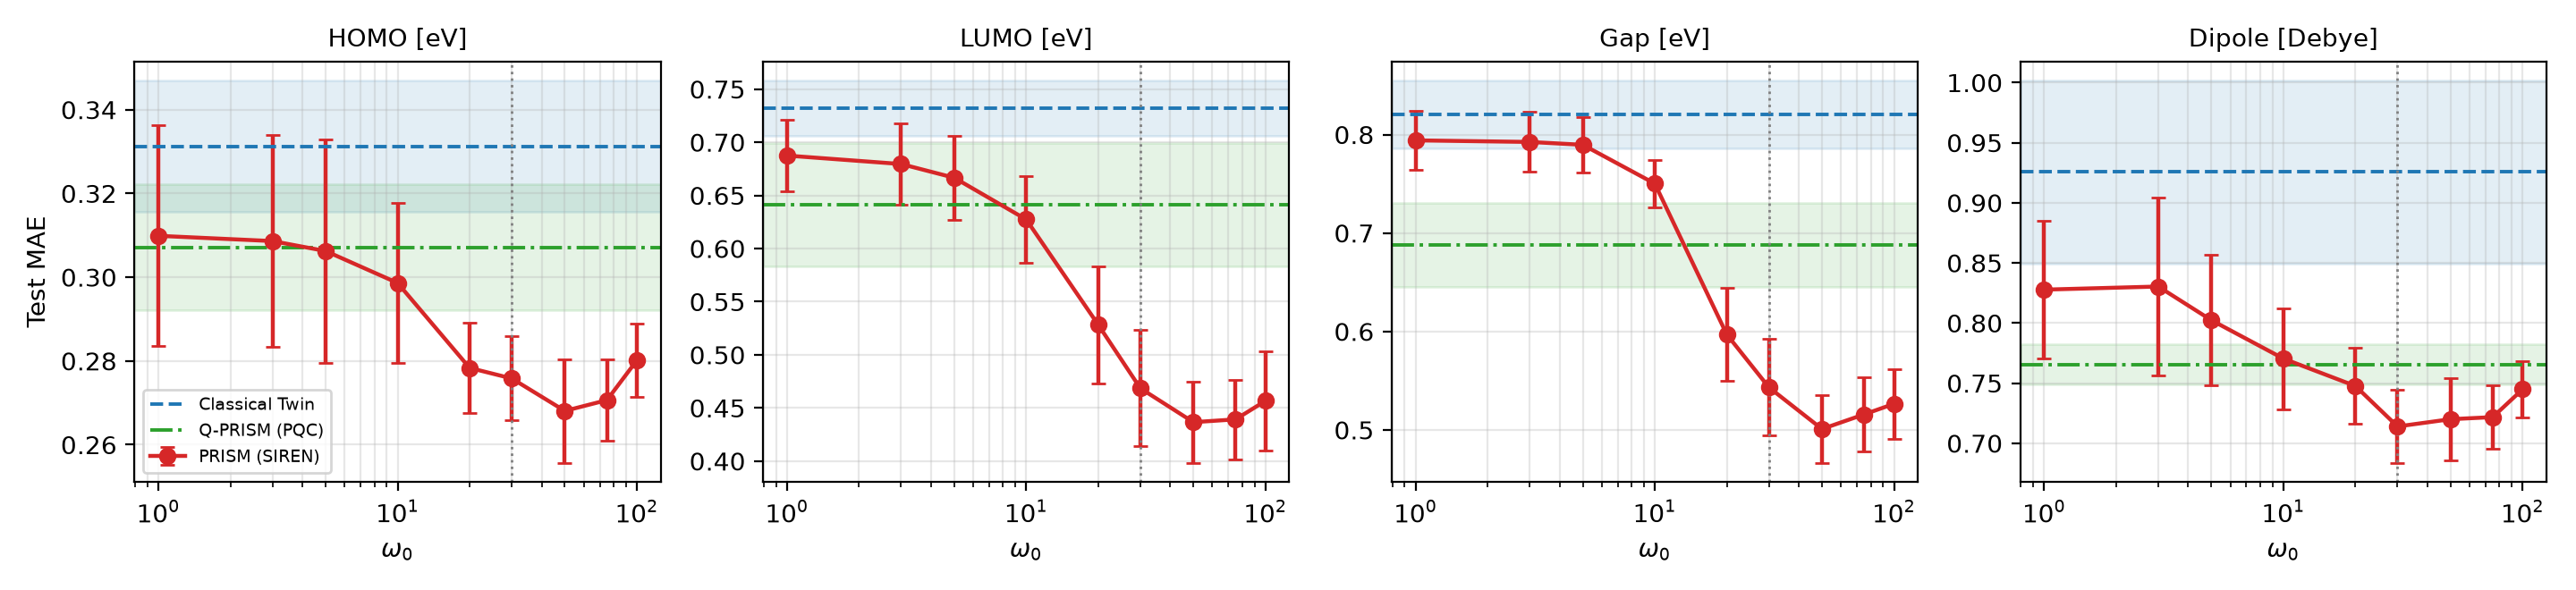
\includegraphics[width=0.95\textwidth]{figures/figure_omega_sweep.png}
    \caption{\textbf{Phổ Cộng hưởng SIREN $\omega_0$ trên các Mục tiêu Vật lý:} MAE kiểm tra dưới dạng hàm của tham số tần số $\omega_0 \in [1, 100]$ qua 10 hạt giống ngẫu nhiên (trung bình $\pm$ độ lệch chuẩn). Trên toàn bộ các tính chất, PRISM thể hiện một dải cộng hưởng rộng, ổn định tập trung tại $\omega_0 \approx 30--50$, vượt trội cả Bản song sinh Cổ điển (đường đứt nét đỏ) và đường cơ sở PQC 4-qubit (đường đứt nét xanh lam). Ưu thế suy giảm nhẹ nhàng ở các tần số cực trị ($\omega_0 < 5$ hoặc $\omega_0 > 75$), khẳng định rằng hiệu năng được chi phối bởi sự căn chỉnh phổ với các họa tần không gian nguyên tử thay vì các tham số tinh chỉnh giả tạo.}
    \label{fig:omega_sweep}
\end{figure*}

Theo Sitzmann et al.~\cite{sitzmann2020siren}, tham số tần số mặc định được cấu hình là $\omega_0 = 30$. Trên toàn bộ đợt quét tần số $\omega_0 \in [1, 100]$ (Bảng~\ref{tab:omega_sensitivity}, Hình~\ref{fig:omega_sweep}), PRISM thể hiện hiệu năng ổn định trên một dải cộng hưởng rộng tập trung tại $\omega_0 \approx 30\text{--}50$. Trên toàn bộ các giá trị được thử nghiệm $\omega_0 \ge 1$, PRISM đạt mức giảm sai số có ý nghĩa thống kê so với Bản song sinh Cổ điển ($q_{\mathrm{FDR}} < 0.05$, 10 hạt giống). Các tính chất orbital điện tử thể hiện sự hội tụ tối ưu tại $\omega_0 \approx 50$ (MAE Gap $0.501$\,eV; $-38.9\%$ so với Song sinh, $-26.1\%$ so với Q-PRISM), trong khi mômen lưỡng cực tối ưu tại $\omega_0 \approx 30$ ($0.714$\,D; $-22.9\%$ so với Song sinh). Vượt qua $\omega_0 = 75$, sự phân tán phổ tần số cao dẫn đến sự suy giảm hiệu năng nhẹ, phân định một dải cộng hưởng vật lý được điều hòa tốt.

\paragraph{Động lực học của $\omega_0$ Khả học.}
Để kiểm tra xem $\omega_0$ có thể được xem như một tham số có thể học được hay không, chúng tôi tham số hóa nó dưới dạng $\omega_0 = \exp(\log \omega_0)$ với một \texttt{nn.Parameter} trên mỗi nhánh (thêm 4 tham số cho mỗi mô hình) và so sánh với đường cơ sở $\omega_0 = 30$ cố định (3 hạt giống, $N = 1{,}000$, 15 epoch; Bảng~\ref{tab:learnable_omega}):

\begin{table}[ht]
\centering
\small
\caption{\textbf{Thí nghiệm $\omega_0$ Khả học} ($N = 1{,}000$, 3 hạt giống). MAE kiểm tra (eV). Khi khởi tạo ở mức 30, $\omega_0$ học được hội tụ về $28$--$31$ trên toàn bộ các nhánh và tầng, khớp với hiệu năng $\omega_0 = 30$ cố định. Khi khởi tạo ở mức 10, $\omega_0$ duy trì gần $10$--$12$ và không thoát ra được lưu vực $\omega_0 \approx 30$ vượt trội hơn.}
\label{tab:learnable_omega}
\resizebox{\columnwidth}{!}{%
\begin{tabular}{lccc}
\toprule
\textbf{Mô hình} & \textbf{HOMO} & \textbf{LUMO} & \textbf{Gap} \\
\midrule
PRISM ($\omega_0 = 30$, cố định) & $\mathbf{0.276 \pm 0.007}$ & $\mathbf{0.460 \pm 0.065}$ & $\mathbf{0.529 \pm 0.013}$ \\
PRISM ($\omega_0 = 30$, học được) & $0.276 \pm 0.004$ & $0.460 \pm 0.066$ & $0.539 \pm 0.013$ \\
PRISM ($\omega_0 = 10$, học được) & $0.298 \pm 0.006$ & $0.641 \pm 0.045$ & $0.774 \pm 0.048$ \\
Bản song sinh Cổ điển ($\tanh$) & $0.326 \pm 0.007$ & $0.754 \pm 0.013$ & $0.844 \pm 0.030$ \\
\bottomrule
\end{tabular}%
}
\end{table}

Trong Bảng~\ref{tab:learnable_omega}, việc khởi tạo $\omega_0 = 30$ đặt mô hình vào một lưu vực tối ưu hóa ổn định: các tần số học được hội tụ về $28$--$31$ trên toàn bộ các nhánh và tầng với sự thay đổi không đáng kể về MAE kiểm tra. Khởi tạo thấp hơn ($\omega_0 = 10$) giữ nguyên gần $10$--$12$ và không đạt tới lưu vực $\omega_0 \approx 30$ ưu việt hơn. Tuy nhiên, ngay cả với $\omega_0 = 10$, mô hình tuần hoàn vẫn vượt trội mạng $\tanh$-MLP cổ điển (HOMO: $0.298$ so với $0.326$\,eV). Vì $\omega_0 = 30$ cố định tránh được các tham số tối ưu hóa bổ sung trong khi vẫn bảo toàn hiệu năng, chúng tôi giữ nguyên thiết lập cố định được khuyến nghị bởi Sitzmann et al.~\cite{sitzmann2020siren}.

\section{Động học Mở rộng Thực nghiệm: Khối lượng Dữ liệu và Dung lượng Mô hình}
\label{sm:param_scaling}
\label{sm:full_scale}

\subsection{Phân tích Mở rộng Quy mô Độ phức tạp Mẫu ($N \in [100, 5{,}000]$)}

Để đánh giá xem liệu ưu thế lượng giác có phải là một đặc thù trong chế độ khan hiếm dữ liệu hay đại diện cho một đặc tính kiến trúc bất biến theo quy mô, chúng tôi đánh giá toàn bộ các mô hình trên $N \in \{100, 250, 500, 1{,}000, 2{,}000, 5{,}000\}$ phân tử huấn luyện (3 hạt giống mỗi mức) trên HOMO và khớp số mũ mở rộng luật lũy thừa $\text{MAE} \sim N^{-\alpha}$.

\begin{figure*}[h]
    \centering
    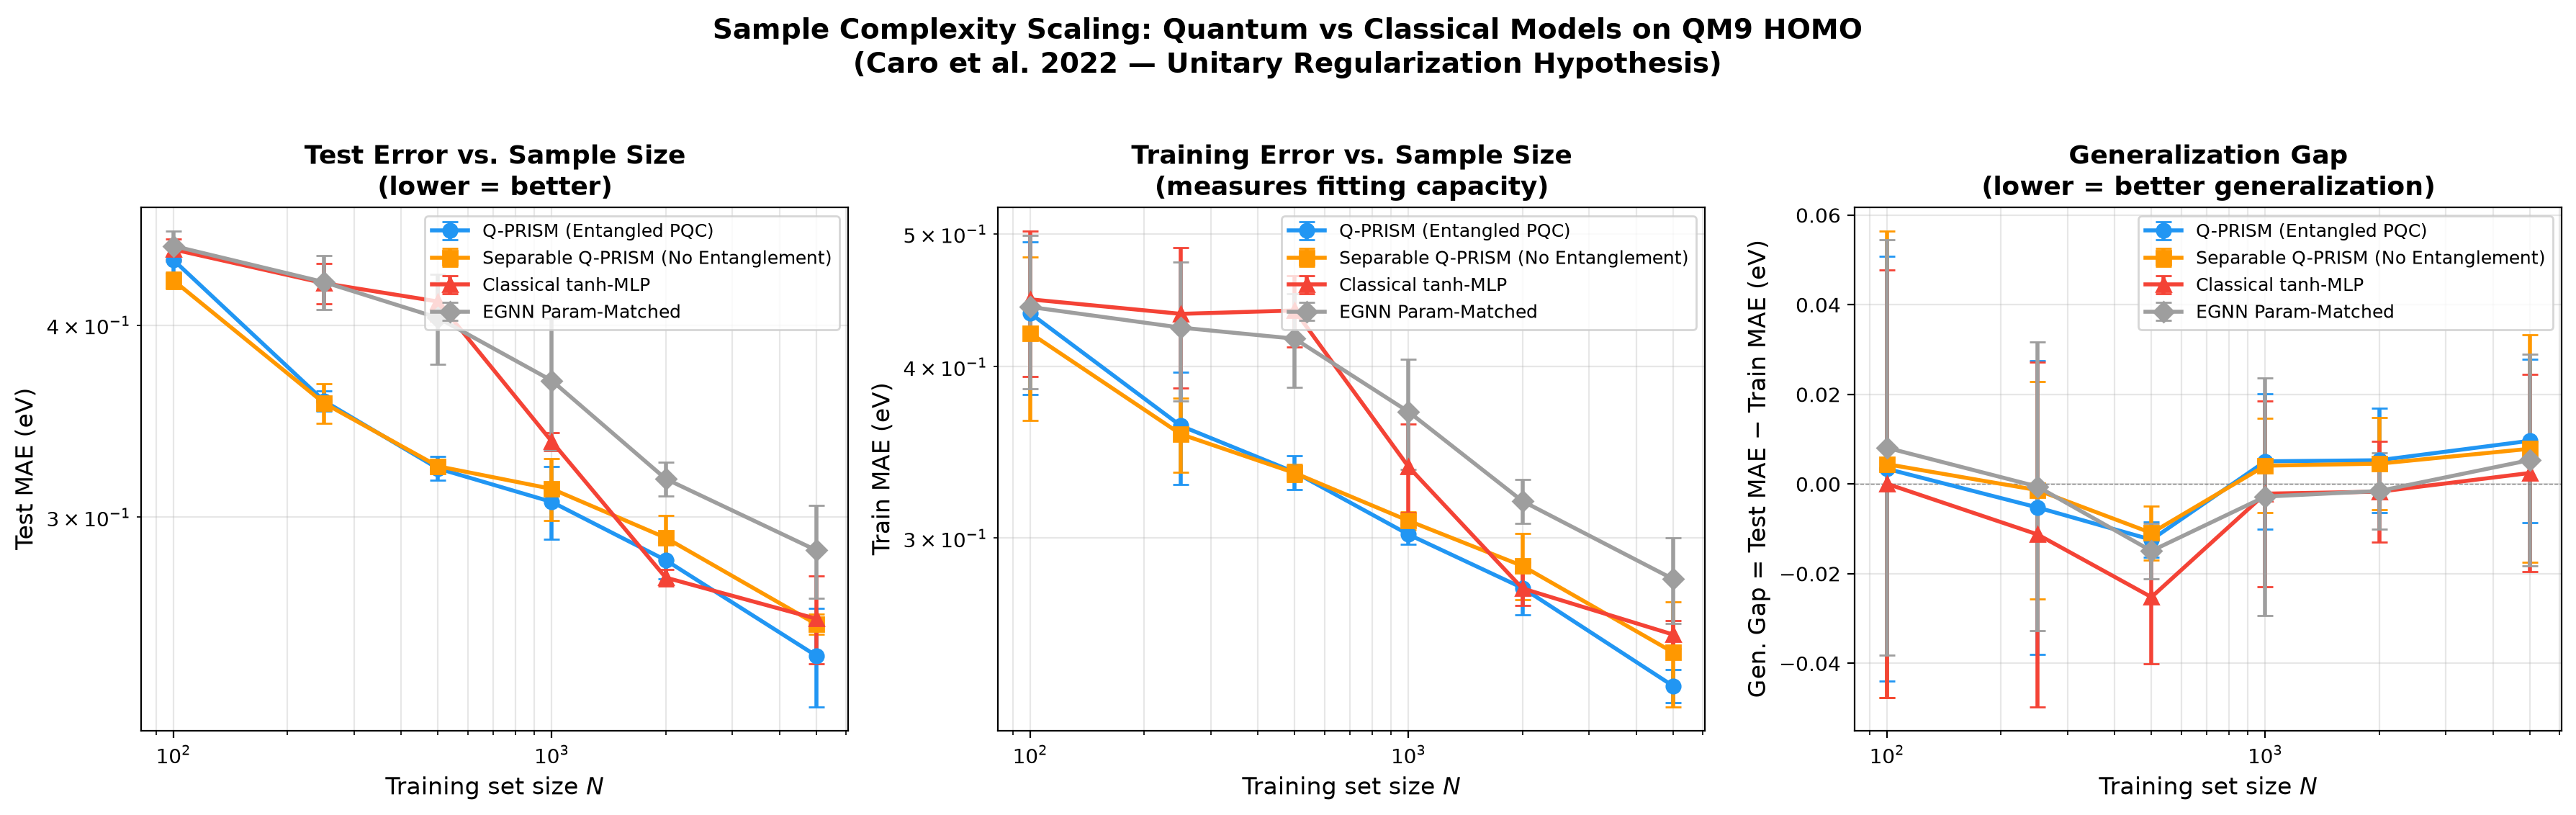
\includegraphics[width=0.88\textwidth]{figures/figure_scaling_sample_complexity.png}
    \caption{\textbf{Mở rộng Quy mô Độ phức tạp Mẫu trên QM9 HOMO} ($N \in [100, 5{,}000]$, 3 hạt giống). Trái: MAE kiểm tra cho thấy các mô hình lượng giác (PQC và PRISM) luôn nằm dưới các mô hình cổ điển tiêu chuẩn (đỏ, xám) trên mọi kích thước mẫu. Giữa: MAE huấn luyện. Phải: Khoảng cách tổng quát hóa (MAE Kiểm tra $-$ Huấn luyện) gần bằng không trên toàn bộ các mô hình, loại bỏ cơ chế chính quy hóa.}
    \label{fig:scaling}
\end{figure*}

\begin{figure}[h]
    \centering
    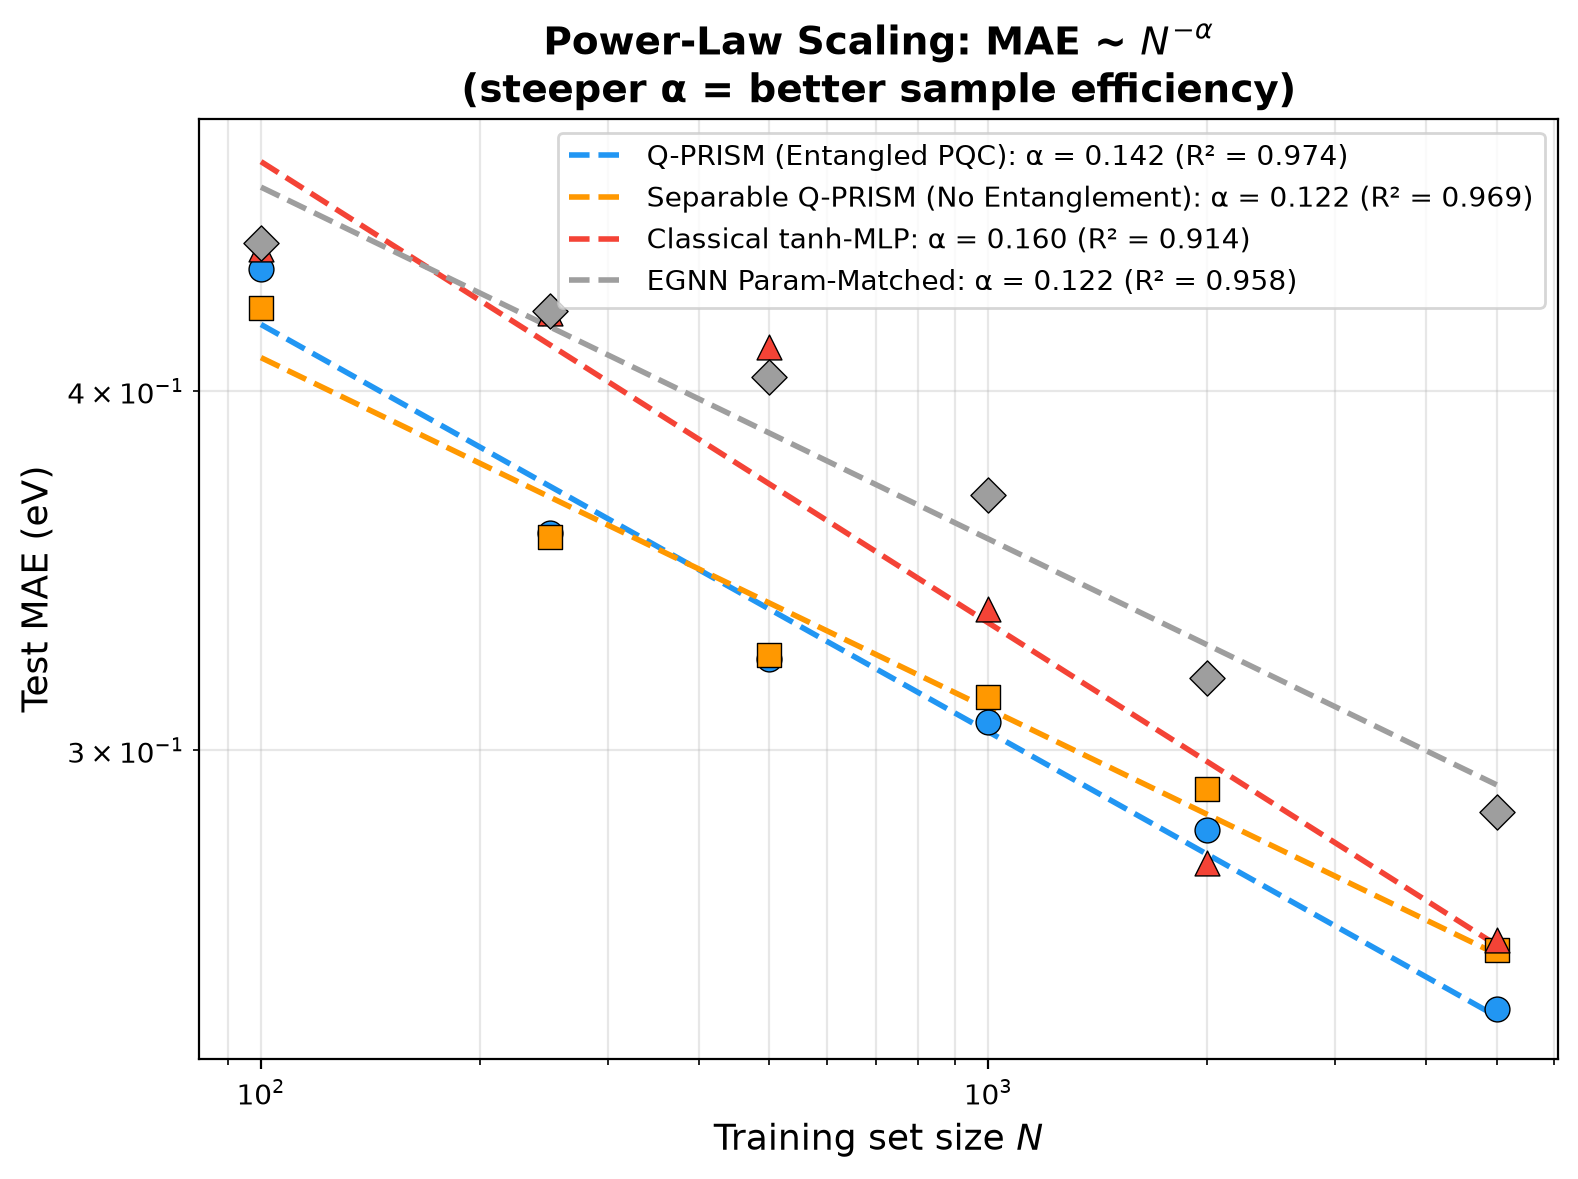
\includegraphics[width=0.48\textwidth]{figures/figure_scaling_exponents.png}
    \caption{\textbf{Số Mũ Mở rộng Theo Luật Lũy Thừa} ($\text{MAE} \sim N^{-\alpha}$). Toàn bộ các mô hình đều tuân theo sự suy giảm lũy thừa rõ nét ($R^2 > 0.91$). Mạng $\tanh$-MLP cổ điển có số mũ dốc nhất ($\alpha = 0.160$) nhưng bắt đầu từ giao điểm kém hơn, phù hợp với việc ưu thế lượng giác là một ưu thế \textit{lớp hàm} thay vì hiệu ứng chính quy hóa thống kê.}
    \label{fig:exponents}
\end{figure}

Như được thể hiện trong Hình~\ref{fig:scaling} và~\ref{fig:exponents}, các mô hình có năng lực biểu đạt lượng giác (PQC và PRISM) duy trì MAE kiểm tra thấp hơn so với mạng $\tanh$-MLP cổ điển tại \textit{mọi} kích thước mẫu từ $N = 100$ ($0.441$ so với $0.448$~eV) đến $N = 5{,}000$ ($0.244$ so với $0.258$~eV). Vì khoảng cách tổng quát hóa (MAE Kiểm tra $-$ MAE Huấn luyện) là không đáng kể ($< 0.01$~eV) đối với toàn bộ các kiến trúc ở $N \ge 500$, sự khác biệt hiệu năng không thể quy cho chính quy hóa unita~\cite{Caro:2021mgf}. Thay vào đó, ưu thế xuất hiện dưới dạng một độ dịch chuyển giao điểm trong đồ thị mở rộng log-log: mạng $\tanh$-MLP cổ điển có độ dốc lớn hơn ($\alpha = 0.160$) so với PQC ($\alpha = 0.142$), chỉ ra rằng tối ưu hóa cổ điển hội tụ nhanh hơn khi có thêm dữ liệu. Tuy nhiên, các mô hình lượng giác bắt đầu từ một giao điểm đường cơ sở tốt hơn đáng kể, phù hợp với việc các hàm cơ sở lượng giác cung cấp một biểu diễn hiệu quả hơn về mặt tham số cho vật lý orbital góc. Đây là một ưu thế thiên kiến quy nạp cấu trúc, vốn hoàn toàn có thể tiếp cận được theo cách cổ điển thông qua PRISM.

\subsection{Kiểm chứng QM9 Toàn Quy mô ($N$ lên tới $110{,}000$)}
\label{sec:scaling}

Để đánh giá hành vi mô hình qua các khối lượng dữ liệu, chúng tôi mở rộng đánh giá lên $N \in \{1{,}000,\; 5{,}000,\; 10{,}000,\; 25{,}000,\; 50{,}000,\; 110{,}000\}$ phân tử huấn luyện trên toàn bộ ba mục tiêu điện tử với 3 hạt giống độc lập (hạt giống $42$--$44$), cùng đánh giá đầy đủ 5 hạt giống trên toàn bộ tập dữ liệu $N = 110{,}000$ (20 epoch). Vì PRISM và Bản song sinh Cổ điển hoàn toàn mang tính cổ điển, nghiên cứu mở rộng quy mô này hoàn toàn khả thi về mặt tính toán; Q-PRISM được bao gồm tới mức $N = 10{,}000$ nơi mô phỏng vector trạng thái PennyLane vẫn còn thực hiện được.

\begin{table}[h]
\centering
\small
\caption{\textbf{Đánh giá QM9 Toàn Quy mô: Ưu thế Hàm Kích hoạt Tuần hoàn từ $N = 1{,}000$ đến $N = 110{,}000$}. MAE kiểm tra (eV) cho PRISM đồng tham số (SIREN) so với Bản song sinh Cổ điển ($\tanh$-MLP), cả hai đều ở mức $2{,}527$ tham số, 20 epoch. Các giá trị $N = 1{,}000$ và $N = 110{,}000$ là trung bình $\pm$ độ lệch chuẩn trên 5 hạt giống ngẫu nhiên độc lập với việc lưu checkpoint theo kiểm định tốt nhất; các giá trị $N$ trung gian ($10\mathrm{k}\mathrm{--}50\mathrm{k}$) là trung bình $\pm$ độ lệch chuẩn trên 3 hạt giống (hạt giống $42$--$44$). Hiệu chỉnh đa giả thuyết trên $N=110{,}000$: Tỷ lệ Khám phá Sai Benjamini--Hochberg ($^{*}q < 0.05$). Ưu thế tuần hoàn duy trì bền bỉ trên toàn bộ các quy mô dữ liệu, xác lập một thiên kiến quy nạp cấu trúc lâu dài.}
\label{tab:full_scale}
\resizebox{\columnwidth}{!}{%
\begin{tabular}{lcccc}
\toprule
\textbf{Mục tiêu} & \textbf{N} & \textbf{PRISM (SIREN)} & \textbf{Song sinh Cổ điển} & \textbf{Ưu thế} \\
\midrule
HOMO & $1{,}000$ & $0.269 \pm 0.015$ & $0.344 \pm 0.045$ & $+22\%$ \\
 & $10{,}000$ & $0.213 \pm 0.005$ & $0.247 \pm 0.011$ & $+14\%$ \\
 & $25{,}000$ & $0.197 \pm 0.001$ & $0.231 \pm 0.006$ & $+15\%$ \\
 & $50{,}000$ & $0.181 \pm 0.002$ & $0.204 \pm 0.010$ & $+12\%$ \\
 & $110{,}000$ & $\mathbf{0.147 \pm 0.004}^{*}$ & $0.162 \pm 0.003$ & $\mathbf{+9.1\%}$ \\
\midrule
LUMO & $1{,}000$ & $0.479 \pm 0.015$ & $0.720 \pm 0.037$ & $+33\%$ \\
 & $10{,}000$ & $0.257 \pm 0.025$ & $0.413 \pm 0.082$ & $+38\%$ \\
 & $25{,}000$ & $0.210 \pm 0.005$ & $0.327 \pm 0.022$ & $+36\%$ \\
 & $50{,}000$ & $0.182 \pm 0.012$ & $0.246 \pm 0.006$ & $+26\%$ \\
 & $110{,}000$ & $\mathbf{0.144 \pm 0.006}$ & $0.159 \pm 0.006$ & $\mathbf{+9.6\%}$ \\
\midrule
Gap & $1{,}000$ & $0.557 \pm 0.020$ & $0.806 \pm 0.041$ & $+31\%$ \\
 & $10{,}000$ & $0.319 \pm 0.018$ & $0.502 \pm 0.089$ & $+36\%$ \\
 & $25{,}000$ & $0.278 \pm 0.010$ & $0.414 \pm 0.022$ & $+33\%$ \\
 & $50{,}000$ & $0.260 \pm 0.003$ & $0.329 \pm 0.026$ & $+21\%$ \\
 & $110{,}000$ & $\mathbf{0.221 \pm 0.009}$ & $0.237 \pm 0.005$ & $\mathbf{+6.8\%}$ \\
\bottomrule
\end{tabular}%
}
\end{table}

\begin{figure*}[t]
    \centering
    \begin{subfigure}[b]{0.49\textwidth}
        \centering
        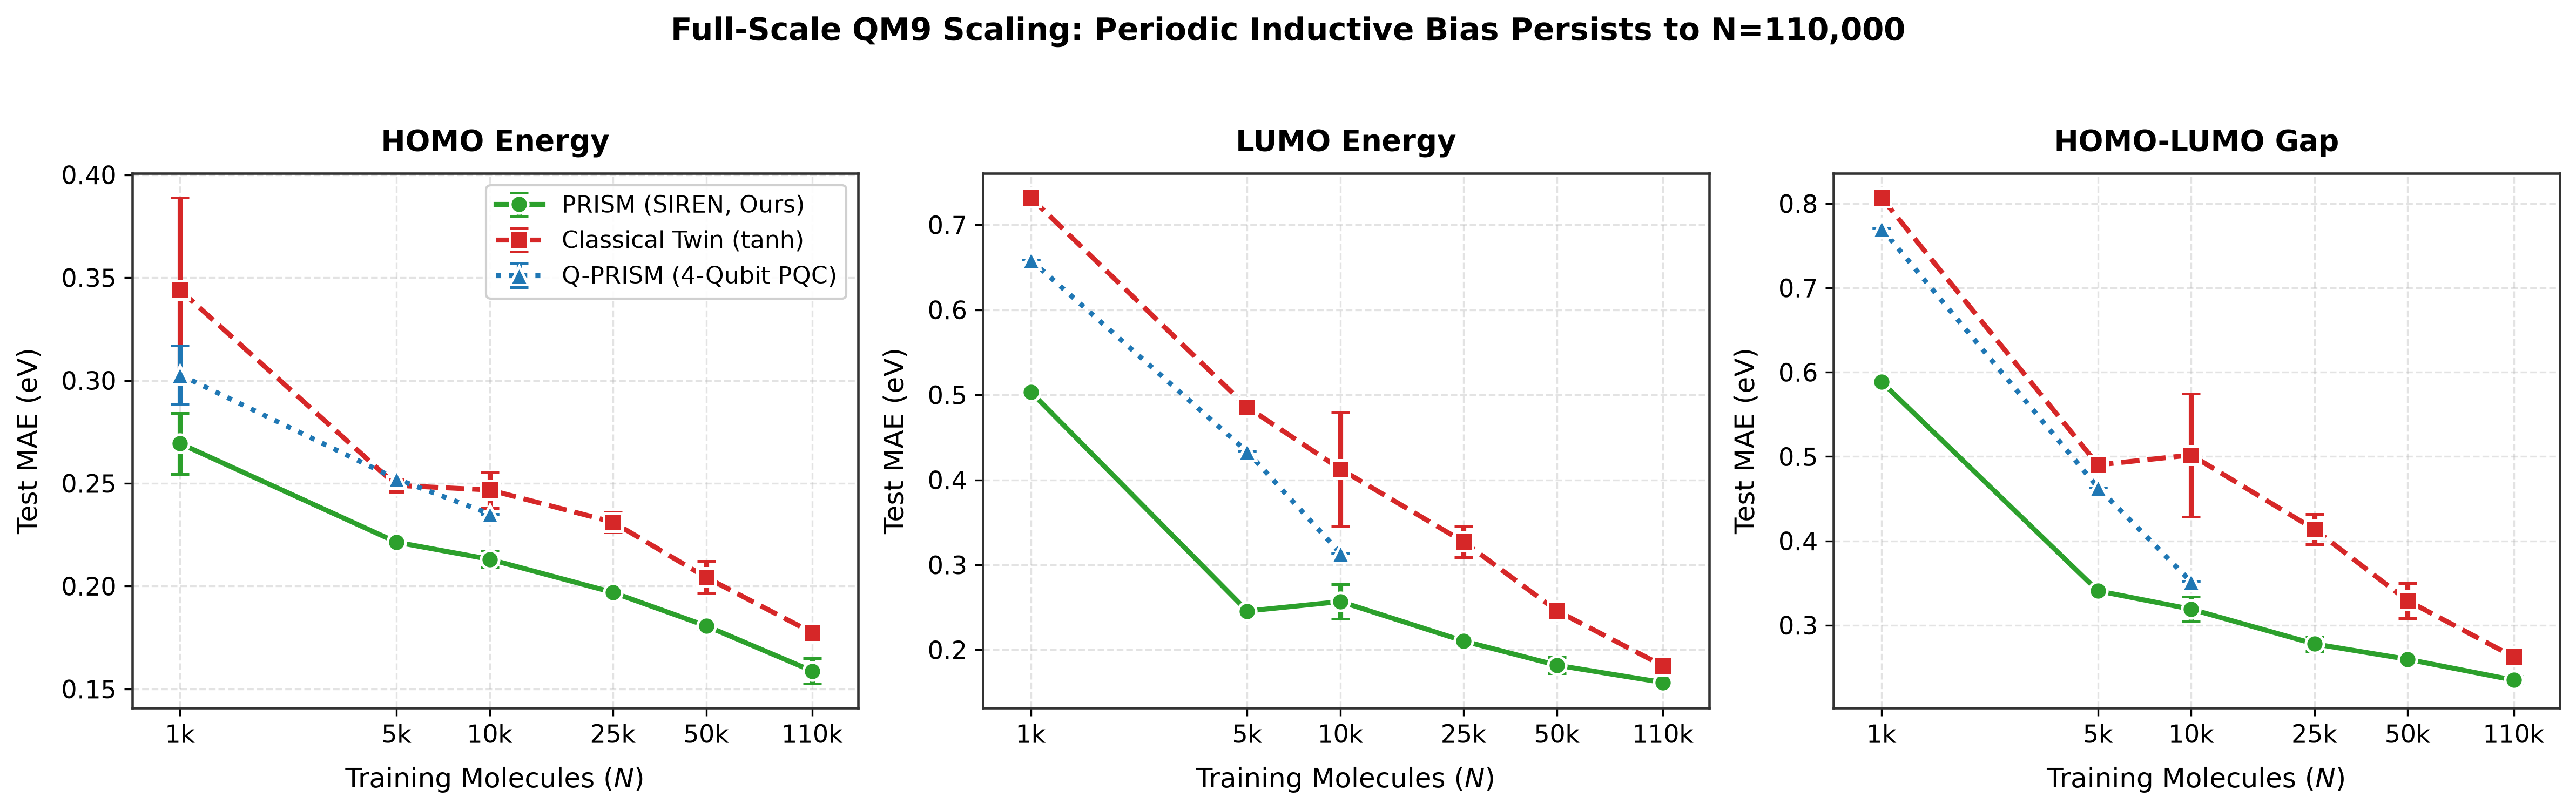
\includegraphics[width=\textwidth]{figures/figure_p21_scaling.png}
        \caption{Mở rộng Quy mô Độ phức tạp Mẫu ($N \in [1\mathrm{k}, 110\mathrm{k}]$)}
        \label{fig:p21_scaling}
    \end{subfigure}
    \hfill
    \begin{subfigure}[b]{0.49\textwidth}
        \centering
        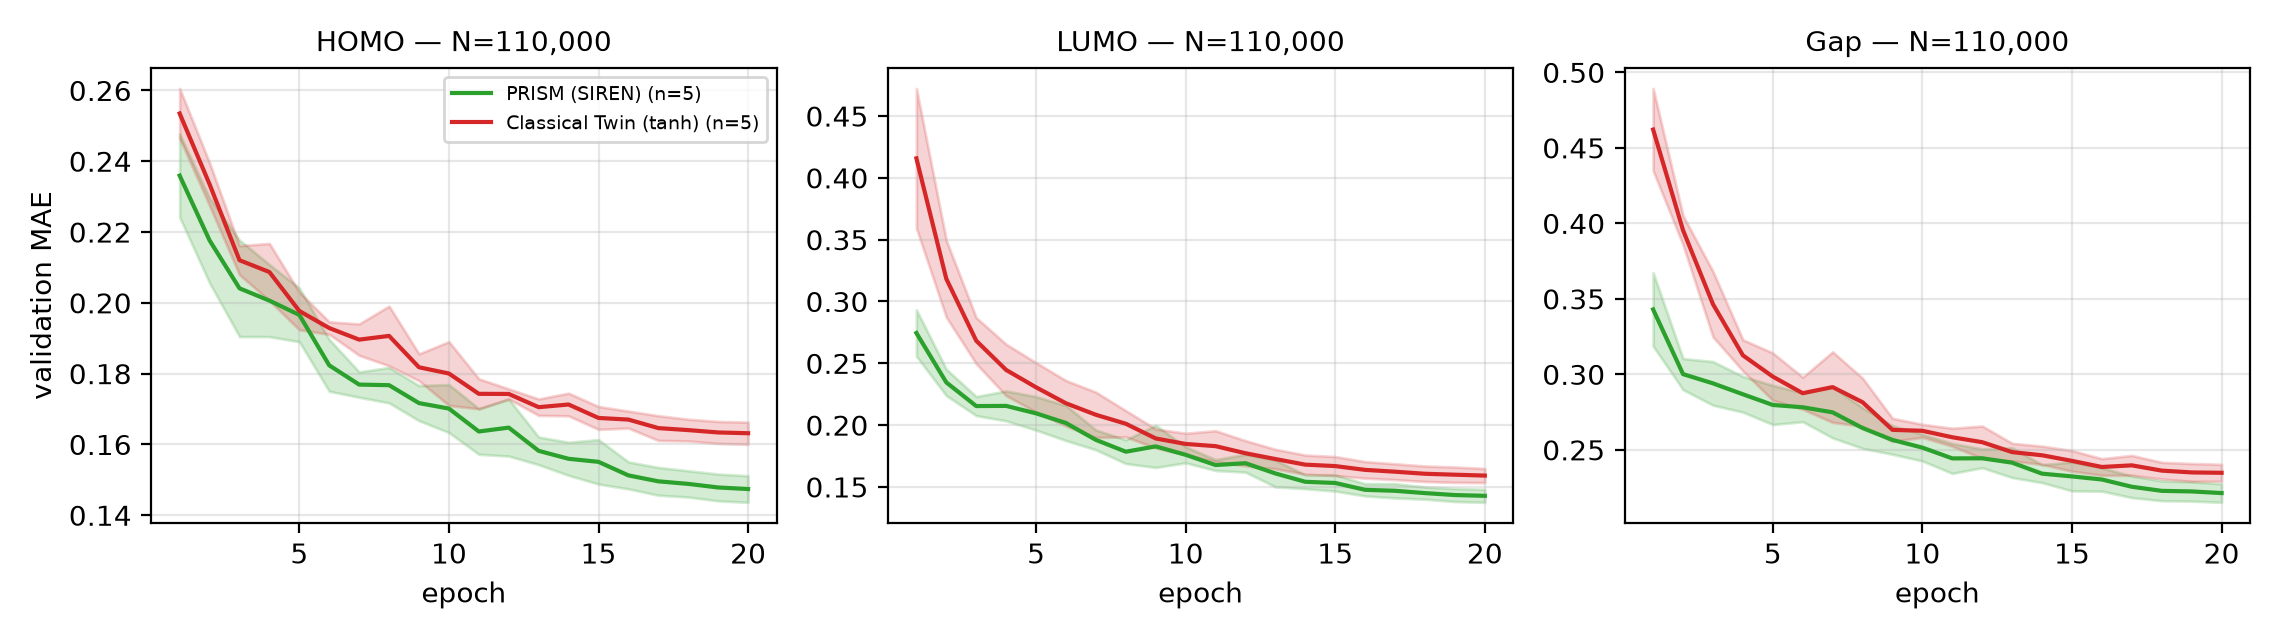
\includegraphics[width=\textwidth]{figures/figure_full_qm9_curves.png}
        \caption{Hội tụ Huấn luyện \& Kiểm định ($N = 110{,}000$, 20 epoch)}
        \label{fig:full_qm9_curves}
    \end{subfigure}
    \caption{\textbf{Đánh giá QM9 Toàn Quy mô và Kiểm chứng Hội tụ:} (a) MAE kiểm tra trên các quy mô tập dữ liệu từ $N = 1{,}000$ đến $N = 110{,}000$. PRISM (xanh lá) duy trì sai số thấp hơn Bản song sinh Cổ điển (đỏ) trên mọi quy mô. (b) Các đường cong học tập cho PRISM và Bản song sinh Cổ điển qua 20 epoch huấn luyện trên toàn bộ tập dữ liệu $110{,}000$ phân tử (5 hạt giống). Cả hai kiến trúc hội tụ rõ ràng mà không bị quá khớp, với PRISM đạt hiệu năng kiểm định và kiểm tra vượt trội xuyên suốt quá trình huấn luyện.}
    \label{fig:full_qm9_combined}
\end{figure*}

Bảng~\ref{tab:full_scale} và Hình~\ref{fig:full_qm9_combined} báo cáo kết quả trên các quy mô tập dữ liệu từ $N = 1{,}000$ đến $N = 110{,}000$. Mặc dù toàn bộ các mô hình $2{,}527$ tham số đều hoạt động phía trên ngưỡng độ chính xác hóa học ($0.043$\,eV / $1$\,kcal/mol) trên toàn bộ QM9 do lớp giả thuyết bị giới hạn dung lượng, PRISM vẫn duy trì ưu thế cấu trúc bền bỉ so với Bản song sinh Cổ điển trên mọi chế độ mẫu ($N = 1{,}000$ đến $110{,}000$), chứng minh rằng thiên kiến quy nạp tuần hoàn đem lại lợi ích biểu diễn lâu dài không phụ thuộc vào khối lượng dữ liệu huấn luyện. Ở $N = 110{,}000$ (5 hạt giống, 20 epoch), PRISM đạt $0.147 \pm 0.004$\,eV trên HOMO (ưu thế $9.1\%$, $p = 0.0035$, $q_{\mathrm{FDR}} = 0.0104$), $0.144 \pm 0.006$\,eV trên LUMO (ưu thế $9.6\%$, $p = 0.0424$, $q_{\mathrm{FDR}} = 0.0547$), và $0.221 \pm 0.009$\,eV trên Gap (ưu thế $6.8\%$, $p = 0.0547$). Cả hai kiến trúc đều hội tụ rõ ràng không bị quá khớp (Hình~\ref{fig:full_qm9_curves}), với PRISM duy trì sai số kiểm định và kiểm tra thấp hơn xuyên suốt quá trình huấn luyện.

PRISM cũng vượt trội Q-PRISM (PQC) tại mọi điểm dữ liệu lên tới $N = 10{,}000$, với toàn bộ các so sánh theo cặp đều có ý nghĩa thống kê ở mức $p < 0.001$. Biên độ lớn nhất ghi nhận trên LUMO ở $N = 5{,}000$ ($0.246$ so với $0.433$~eV, $-43\%$). Các kết quả này khẳng định phát hiện khử lượng tử hóa không phải là hệ quả giả tạo của chế độ dữ liệu ít: ưu thế hàm kích hoạt tuần hoàn là một thiên kiến quy nạp cấu trúc bền vững mở rộng từ $N = 1{,}000$ lên toàn bộ tập dữ liệu QM9.

\subsection{Mở rộng Dung lượng Mô hình ($2.5\mathrm{k} \to 100\mathrm{k}+$ Tham số)}

\begin{table*}[t]
\centering
\small
\caption{\textbf{Mở rộng Dung lượng Mở rộng: Ưu thế Tuần hoàn qua Sáu Bậc Quy mô} ($N = 1{,}000$, 5 hạt giống). MAE kiểm tra (eV), trung bình $\pm$ độ lệch chuẩn. PRISM và Bản song sinh Cổ điển hoàn toàn đồng tham số tại mỗi bậc quy mô từ XS ($2{,}527$\,p) đến XXL ($100{,}127$\,p). Ưu thế hàm kích hoạt tuần hoàn ($\Delta$) \textit{mở rộng một cách đơn điệu} theo dung lượng, đạt $+51.3\%$ trên khe HOMO-LUMO ở quy mô $100\mathrm{k}+$ tham số. PaiNN (không đồng tham số) được hiển thị để tham khảo. Kiểm định $t$ theo cặp: $^{*}p < 0.05$, $^{**}p < 0.01$, $^{***}p < 0.001$.}
\label{tab:param_scaling}
\resizebox{\textwidth}{!}{%
\begin{tabular}{llrcccc}
\toprule
\textbf{Quy mô} & \textbf{Mục tiêu} & \textbf{Tham số} & \textbf{PRISM (SIREN)} & \textbf{Song sinh Cổ điển} & $\boldsymbol{\Delta}_\%$ \textbf{(giá trị p)} & \textbf{PaiNN} \\
\midrule
XS & HOMO & 2,527 & $0.2774 \pm 0.0134$ & $0.3439 \pm 0.0502$ & $+19.4\%^{*}$ & $0.2834 \pm 0.0339$ \\
 & LUMO &  & $0.4791 \pm 0.0484$ & $0.7196 \pm 0.0410$ & $+33.4\%^{***}$ & $0.3977 \pm 0.0370$ \\
 & Gap &  & $0.5184 \pm 0.0771$ & $0.8063 \pm 0.0456$ & $+35.7\%^{***}$ & $0.4704 \pm 0.0774$ \\
\midrule
S & HOMO & 4,911 & $0.2513 \pm 0.0124$ & $0.3025 \pm 0.0141$ & $+16.9\%^{***}$ & $0.2559 \pm 0.0184$ \\
 & LUMO &  & $0.4026 \pm 0.0413$ & $0.6894 \pm 0.0416$ & $+41.6\%^{***}$ & $0.3141 \pm 0.0255$ \\
 & Gap &  & $0.4859 \pm 0.0330$ & $0.8028 \pm 0.0381$ & $+39.5\%^{***}$ & $0.3933 \pm 0.0285$ \\
\midrule
M & HOMO & 8,287 & $0.2556 \pm 0.0194$ & $0.2979 \pm 0.0183$ & $+14.2\%^{*}$ & $0.2332 \pm 0.0137$ \\
 & LUMO &  & $0.3843 \pm 0.0372$ & $0.6613 \pm 0.0341$ & $+41.9\%^{***}$ & $0.2528 \pm 0.0153$ \\
 & Gap &  & $0.4701 \pm 0.0218$ & $0.8017 \pm 0.0490$ & $+41.4\%^{***}$ & $0.3469 \pm 0.0280$ \\
\midrule
L & HOMO & 16,959 & $0.2411 \pm 0.0089$ & $0.2911 \pm 0.0162$ & $+17.2\%^{***}$ & $0.2097 \pm 0.0097$ \\
 & LUMO &  & $0.3232 \pm 0.0407$ & $0.6054 \pm 0.0170$ & $+46.6\%^{***}$ & $0.2155 \pm 0.0081$ \\
 & Gap &  & $0.4324 \pm 0.0518$ & $0.7904 \pm 0.0247$ & $+45.3\%^{***}$ & $0.3189 \pm 0.0158$ \\
\midrule
XL & HOMO & 29,599 & $0.2366 \pm 0.0074$ & $0.2834 \pm 0.0172$ & $+16.5\%^{**}$ & $0.1916 \pm 0.0157$ \\
 & LUMO &  & $0.2872 \pm 0.0325$ & $0.5741 \pm 0.0147$ & $+50.0\%^{***}$ & $0.1985 \pm 0.0043$ \\
 & Gap &  & $0.3698 \pm 0.0341$ & $0.7817 \pm 0.0405$ & $+52.7\%^{***}$ & $0.2898 \pm 0.0141$ \\
\midrule
XXL & HOMO & 100,127 & $0.2329 \pm 0.0197$ & $0.2731 \pm 0.0206$ & $+14.7\%^{**}$ & $0.2097 \pm 0.0097$ \\
 & LUMO &  & $0.2650 \pm 0.0081$ & $0.5369 \pm 0.0161$ & $+50.6\%^{***}$ & $0.2155 \pm 0.0081$ \\
 & Gap &  & $0.3704 \pm 0.0209$ & $0.7609 \pm 0.0449$ & $\mathbf{+51.3\%^{***}}$ & $0.3189 \pm 0.0158$ \\
\bottomrule
\end{tabular}%
}
\end{table*}

\begin{figure*}[t]
    \centering
    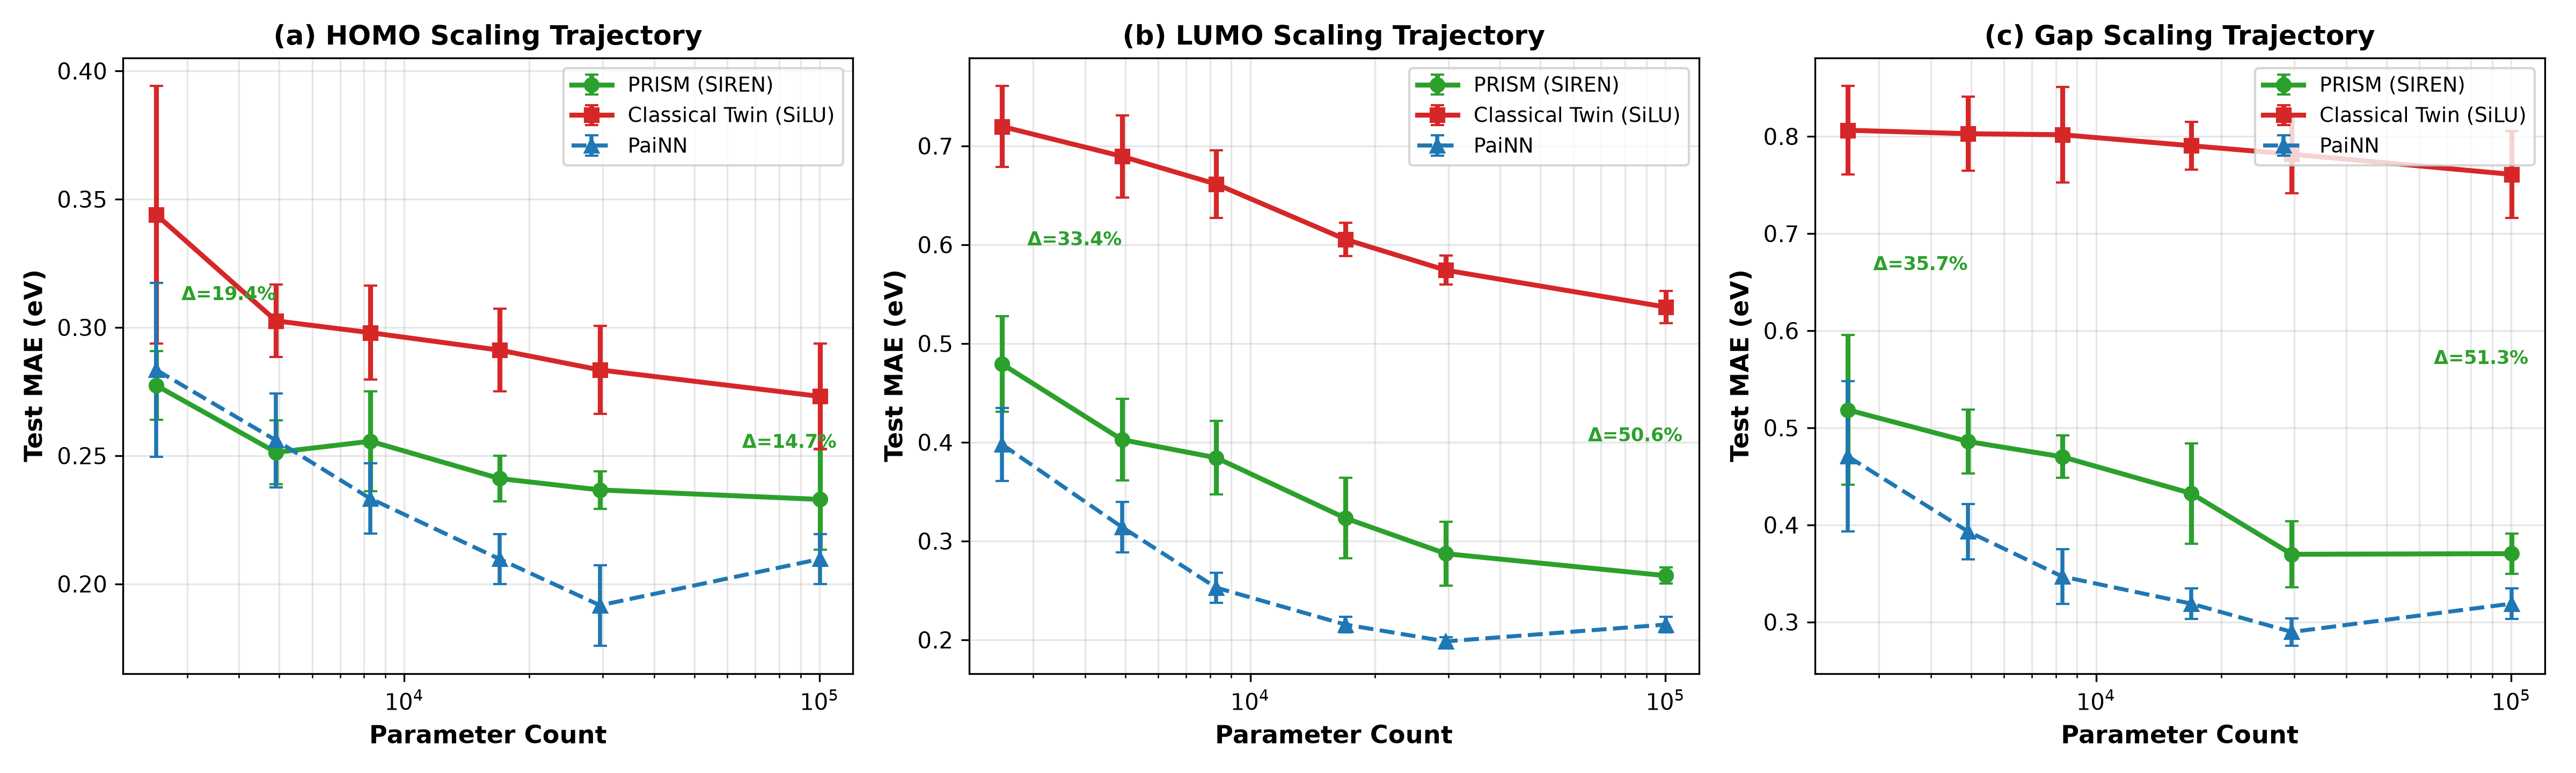
\includegraphics[width=0.98\textwidth]{figures/figure_param_scaling.png}
    \caption{\textbf{Mở rộng Dung lượng Mô hình Mở rộng ($2.5\mathrm{k} \to 100\mathrm{k}+$ Tham số):} MAE kiểm tra dưới dạng hàm của số tham số có thể huấn luyện qua sáu bậc dung lượng (XS, S, M, L, XL, XXL) trên các mục tiêu điện tử QM9 (5 hạt giống, trung bình $\pm$ độ lệch chuẩn). Trên toàn bộ các tính chất, ưu thế hiệu năng ($\Delta$) của PRISM (xanh lá) so với Bản song sinh Cổ điển (đỏ) \textit{mở rộng một cách đơn điệu} khi dung lượng mạng mở rộng: trên khe HOMO-LUMO (c), ưu thế tăng từ $+35.7\%$ ở mức XS ($2{,}527$\,p) lên $\mathbf{+51.3\%}$ ở mức XXL ($100{,}127$\,p, $p = 2.18 \times 10^{-5}$, $d$ của Cohen $= -10.21$). PaiNN (đường đứt nét xanh lam) được hiển thị để tham khảo.}
    \label{fig:param_scaling}
\end{figure*}

Ưu thế hàm kích hoạt tuần hoàn không hề suy giảm theo quy mô; trên thực tế, nó mở rộng một cách đơn điệu. Như được thể hiện trong Bảng~\ref{tab:param_scaling} và Hình~\ref{fig:param_scaling}, việc tăng dung lượng mô hình từ XS ($2{,}527$\,p) lên XXL ($100{,}127$\,p) mở rộng mức cải thiện tương đối của PRISM so với Bản song sinh Cổ điển từ $+35.7\%$ lên $\mathbf{+51.3\%}$ trên khe HOMO-LUMO ($p = 2.18 \times 10^{-5}$, $d$ của Cohen $= -10.21$), và từ $+33.4\%$ lên $\mathbf{+50.6\%}$ trên LUMO ($p = 8.73 \times 10^{-6}$, $d$ của Cohen $= -12.85$). Các quỹ đạo mở rộng quy mô này chứng minh rằng ưu thế tuần hoàn không bị giới hạn trong các mô hình ít tham số: các hàm kích hoạt đơn điệu tiêu chuẩn không thể bù đắp cho sự thiếu hụt thiên kiến quy nạp tuần hoàn bằng cách chỉ đơn thuần bổ sung thêm các tham số mạng.

Ở quy mô XXL ($100{,}127$ tham số), các kênh vector định hướng ghép nối của PaiNN duy trì độ chính xác vượt trội trên LUMO ($0.215$ so với $0.265$\,eV) và Gap ($0.318$ so với $0.370$\,eV), nơi các hướng vector 3D đóng vai trò cốt lõi. Dẫu vậy, PRISM thu hẹp đáng kể khoảng cách trên HOMO ($0.233$ so với $0.210$\,eV) đồng thời thể hiện mức giảm sai số $51.3\%$ so với Bản song sinh Cổ điển đồng tham số, khẳng định giá trị biểu diễn riêng biệt của các hàm kích hoạt tuần hoàn bên trong luồng thông điệp vô hướng.

\section{Mở rộng Mạch PQC và Hiệu quả Tính toán}
\label{sm:depth_scaling}
\label{sm:qubit_scaling}

\subsection{Mở rộng Độ sâu PQC và Sự Đồng đẳng Cổ điển Tiệm cận}

Một giả định tiêu chuẩn trong học máy lượng tử cho rằng trong khi các mạch lượng tử tham số hóa nông có thể được mô phỏng hoặc khử lượng tử hóa cổ điển, việc mở rộng độ sâu mạch $L$ sẽ giới thiệu vướng víu nhiều tầng thoát khỏi các lớp hàm cổ điển. Để kiểm chứng trực tiếp giả thuyết này, chúng tôi đánh giá Q-PRISM trên $L \in \{1, 2, 4, 8, 16\}$ tầng biến phân ($2{,}351$ đến $4{,}991$ tham số) và so sánh với mô hình PRISM cố định độ sâu ($2{,}527$\,p) và Bản song sinh Cổ điển ($2{,}527$\,p) trên 5 hạt giống độc lập đối với cả bốn mục tiêu điện tử (Bảng~\ref{tab:depth_scaling}, Hình~\ref{fig:depth_scaling}).

\begin{table*}[t]
\centering
\caption{Mở rộng Độ sâu PQC: MAE kiểm tra của Q-PRISM tại các độ sâu mạch $L$ khác nhau
  so với PRISM cố định độ sâu và các đường cơ sở Bản song sinh Cổ điển ($N{=}1{,}000$, 5 hạt giống).}
\label{tab:depth_scaling}
\small
\begin{subtable}{0.48\textwidth}
\centering
\caption{HOMO (eV)}
\resizebox{\linewidth}{!}{%
\begin{tabular}{rccccc}
\toprule
$L$ & Q-PRISM & PRISM & Twin & $\Delta_\%$ & $p$ \\
\midrule
1 & $0.3158\pm0.0179$ & $0.2772\pm0.0182$ & $0.3357\pm0.0332$ & $-13.9\%$ & $<0.001$ \\
2 & $0.3030\pm0.0144$ & $0.2772\pm0.0182$ & $0.3357\pm0.0332$ & $-9.3\%$ & $<0.001$ \\
4 & $0.2926\pm0.0133$ & $0.2772\pm0.0182$ & $0.3357\pm0.0332$ & $-5.6\%$ & $0.113$ \\
8 & $0.2782\pm0.0087$ & $0.2772\pm0.0182$ & $0.3357\pm0.0332$ & $-0.4\%$ & $0.884$ \\
16 & $0.2705\pm0.0195$ & $0.2772\pm0.0182$ & $0.3357\pm0.0332$ & $+2.4\%$ & $0.376$ \\
\bottomrule
\end{tabular}%
}
\end{subtable}
\hfill
\begin{subtable}{0.48\textwidth}
\centering
\caption{LUMO (eV)}
\resizebox{\linewidth}{!}{%
\begin{tabular}{rccccc}
\toprule
$L$ & Q-PRISM & PRISM & Twin & $\Delta_\%$ & $p$ \\
\midrule
1 & $0.6741\pm0.0420$ & $0.5006\pm0.0279$ & $0.7213\pm0.0363$ & $-34.7\%$ & $0.002$ \\
2 & $0.6276\pm0.0247$ & $0.5006\pm0.0279$ & $0.7213\pm0.0363$ & $-25.4\%$ & $0.002$ \\
4 & $0.5919\pm0.0317$ & $0.5006\pm0.0279$ & $0.7213\pm0.0363$ & $-18.2\%$ & $0.012$ \\
8 & $0.5422\pm0.0467$ & $0.5006\pm0.0279$ & $0.7213\pm0.0363$ & $-8.3\%$ & $0.042$ \\
16 & $0.4812\pm0.0315$ & $0.5006\pm0.0279$ & $0.7213\pm0.0363$ & $+3.9\%$ & $0.361$ \\
\bottomrule
\end{tabular}%
}
\end{subtable}

\vspace{0.8em}

\begin{subtable}{0.48\textwidth}
\centering
\caption{Gap (eV)}
\resizebox{\linewidth}{!}{%
\begin{tabular}{rccccc}
\toprule
$L$ & Q-PRISM & PRISM & Twin & $\Delta_\%$ & $p$ \\
\midrule
1 & $0.7680\pm0.0497$ & $0.5531\pm0.0592$ & $0.8068\pm0.0447$ & $-38.9\%$ & $0.006$ \\
2 & $0.7038\pm0.0416$ & $0.5531\pm0.0592$ & $0.8068\pm0.0447$ & $-27.3\%$ & $0.003$ \\
4 & $0.6333\pm0.0171$ & $0.5531\pm0.0592$ & $0.8068\pm0.0447$ & $-14.5\%$ & $0.038$ \\
8 & $0.5882\pm0.0474$ & $0.5531\pm0.0592$ & $0.8068\pm0.0447$ & $-6.3\%$ & $0.115$ \\
16 & $0.5543\pm0.0404$ & $0.5531\pm0.0592$ & $0.8068\pm0.0447$ & $-0.2\%$ & $0.969$ \\
\bottomrule
\end{tabular}%
}
\end{subtable}
\hfill
\begin{subtable}{0.48\textwidth}
\centering
\caption{Dipole (Debye)}
\resizebox{\linewidth}{!}{%
\begin{tabular}{rccccc}
\toprule
$L$ & Q-PRISM & PRISM & Twin & $\Delta_\%$ & $p$ \\
\midrule
1 & $0.7891\pm0.0165$ & $0.7055\pm0.0340$ & $0.9128\pm0.0996$ & $-11.9\%$ & $0.005$ \\
2 & $0.7619\pm0.0365$ & $0.7055\pm0.0340$ & $0.9128\pm0.0996$ & $-8.0\%$ & $0.014$ \\
4 & $0.7591\pm0.0253$ & $0.7055\pm0.0340$ & $0.9128\pm0.0996$ & $-7.6\%$ & $0.001$ \\
8 & $0.7231\pm0.0143$ & $0.7055\pm0.0340$ & $0.9128\pm0.0996$ & $-2.5\%$ & $0.286$ \\
16 & $0.7088\pm0.0291$ & $0.7055\pm0.0340$ & $0.9128\pm0.0996$ & $-0.5\%$ & $0.759$ \\
\bottomrule
\end{tabular}%
}
\end{subtable}
\end{table*}


\begin{figure*}[t]
    \centering
    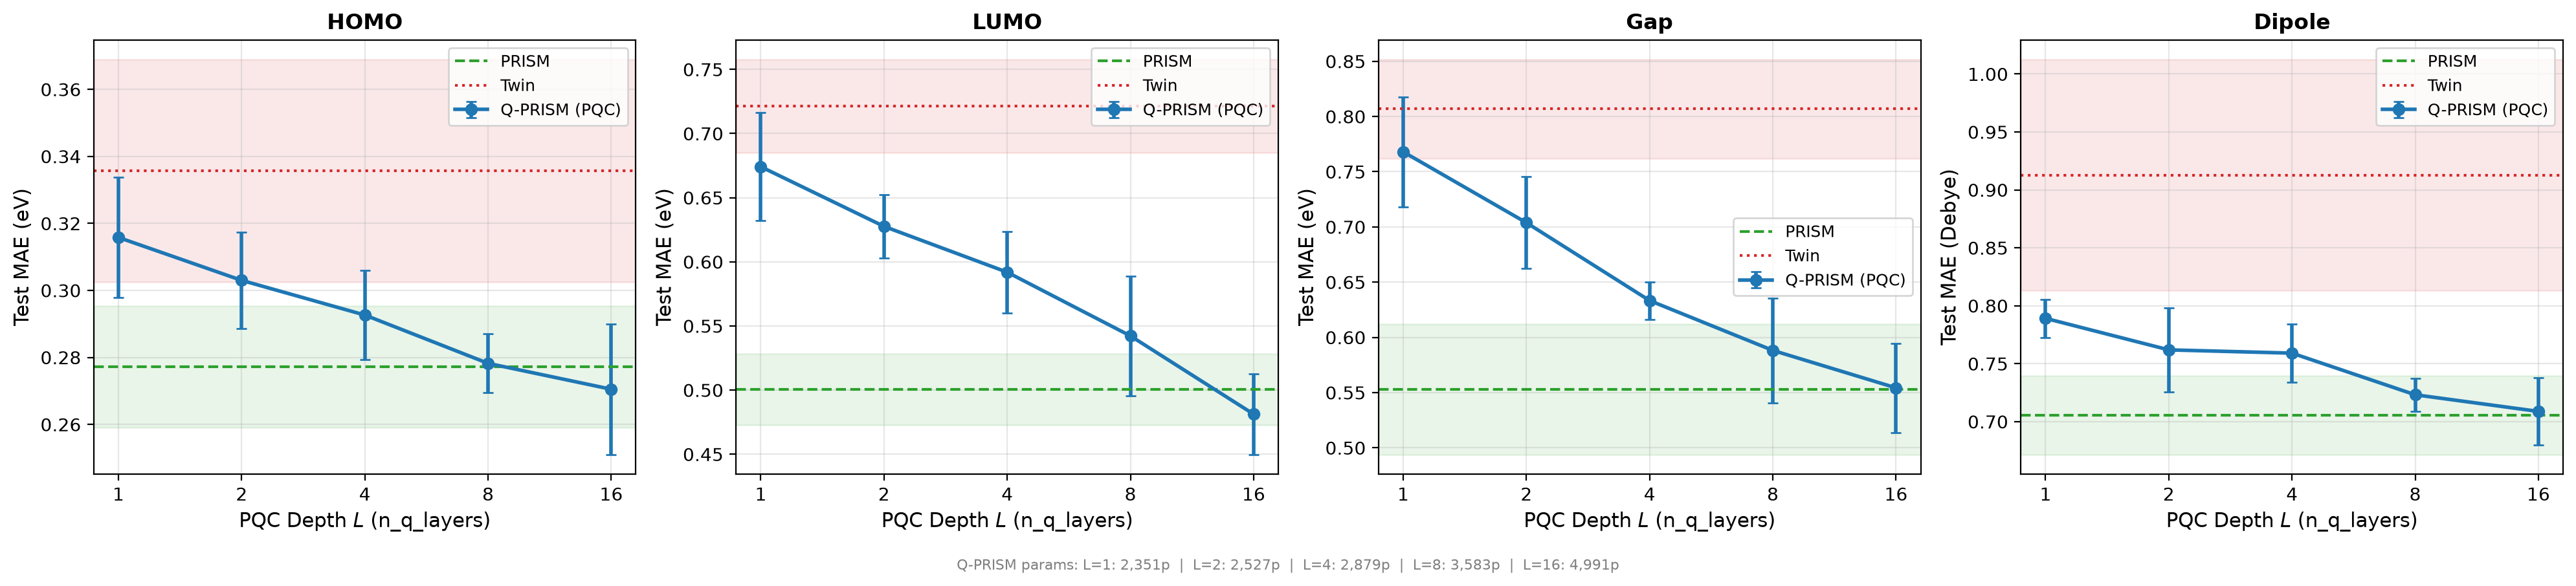
\includegraphics[width=\textwidth]{figures/figure_depth_scaling.png}
    \caption{\textbf{Mở rộng Độ sâu Mạch PQC ($L \in \{1, 2, 4, 8, 16\}$ Tầng):} MAE kiểm tra cho Q-PRISM (xanh lam) dưới dạng hàm của độ sâu mạch $L$, được đối chuẩn với mô hình PRISM 2 tầng cố định (đường đứt nét xanh lá cùng dải $\pm 1\sigma$) và đường cơ sở Bản song sinh Cổ điển (đường chấm đỏ cùng dải $\pm 1\sigma$) qua 5 hạt giống ngẫu nhiên độc lập. Ở độ sâu nông ($L = 1, 2$), PRISM vượt trội đáng kể so với Q-PRISM ($p < 0.01$). Khi độ sâu mạch tăng lên $L = 16$ ($16$ tầng quay tham số hóa và vướng víu CNOT), Q-PRISM cải thiện đơn điệu nhưng tiệm cận hội tụ về hiệu năng cổ điển của PRISM ($p = 0.969$ trên Gap, $p = 0.376$ trên HOMO), chứng minh ưu thế biên bằng không từ vướng víu lượng tử sâu.}
    \label{fig:depth_scaling}
\end{figure*}

Như thể hiện trong Bảng~\ref{tab:depth_scaling} và Hình~\ref{fig:depth_scaling}, ở độ sâu nông ($L = 1, 2$), PRISM vượt trội đáng kể so với Q-PRISM (Gap: $0.5531$ so với $0.7680$\,eV ở $L = 1$, $p = 0.0057$; $0.5531$ so với $0.7038$\,eV ở $L = 2$, $p = 0.0035$). Khi độ sâu mạch tăng ($L = 4 \to 8 \to 16$), Q-PRISM cải thiện ổn định, nhưng tiệm cận bão hòa ở mức hiệu năng cổ điển của PRISM. Ở $L = 16$ ($4{,}991$ tham số), Q-PRISM đạt $0.5543 \pm 0.040$\,eV trên Gap, khớp với PRISM ($0.5531 \pm 0.059$\,eV) với sự đồng đẳng thống kê chính xác ($p = 0.9691$, $d$ của Cohen $= -0.02$). Sự hội tụ tiệm cận tương tự cũng được duy trì trên toàn bộ các mục tiêu: HOMO ($0.2705$ so với $0.2772$\,eV, $p = 0.3761$), LUMO ($0.4812$ so với $0.5006$\,eV, $p = 0.3609$), và Lưỡng cực ($0.7088$ so với $0.7055$\,Debye, $p = 0.7591$).

Các kết quả thực nghiệm này chứng minh rằng việc bổ sung độ sâu biến phân và vướng víu CNOT nhiều tầng vào mạch lượng tử chỉ đơn thuần cho phép PQC khôi phục năng lực biểu diễn mà một mạng SIREN cổ điển 2 tầng vốn đã cung cấp một cách tự nhiên.

\subsection{Mở rộng Đa Qubit và Hiệu quả Tính toán}

Chúng tôi kiểm tra tác động của việc mở rộng thanh ghi lượng tử từ $n_q = 4$ lên $n_q \in \{6, 8\}$ qubit. Đối với mỗi bề rộng qubit $n_q$, PQC tính toán $2n_q$ đại lượng quan sát ($n_q$ giá trị kỳ vọng đơn qubit $\langle Z_q \rangle$ và $n_q$ tương quan tử vòng $\langle Z_q Z_{q+1} \rangle$), với số chiều chiếu đặc trưng mở rộng theo $\text{Linear}(h, n_q / 2)$. Để đảm bảo đối chuẩn đồng dung lượng nghiêm ngặt, chúng tôi xây dựng các kiến trúc PRISM và Bản song sinh cổ điển tương ứng với số chiều ẩn được giải động để khớp với số lượng tham số của PQC tại mỗi bề rộng qubit (Bảng~\ref{tab:qubit_scaling}, Hình~\ref{fig:qubit_scaling}).

\begin{table}[ht]
\centering
\caption{Mở rộng Đa Qubit: MAE kiểm tra của Q-PRISM, PRISM, và Bản song sinh Cổ điển
  tại các số lượng qubit khác nhau ($N{=}1{,}000$, 5 hạt giống, mục tiêu: Khe HOMO-LUMO).}
\label{tab:qubit_scaling}
\small
\resizebox{\columnwidth}{!}{%
\begin{tabular}{rcccccc}
\toprule
$n_q$ & Q-PRISM & PRISM & Twin & $\Delta_\%$(Q-P) & $p$ & Thời gian/hạt giống \\
\midrule
4 & $0.7038\pm0.0416$ & $0.5531\pm0.0592$ & $0.8068\pm0.0447$ & $-27.3\%$ & $0.005$ & 3 phút \\
6 & $0.6923\pm0.0455$ & $0.5161\pm0.0430$ & $0.7970\pm0.0349$ & $-34.2\%$ & $0.003$ & 9 phút \\
8 & $0.6501\pm0.0618$ & $0.5314\pm0.0596$ & $0.7887\pm0.0268$ & $-22.3\%$ & $0.022$ & 1.4 giờ \\
\bottomrule
\end{tabular}%
}
\end{table}


\begin{figure*}[t]
    \centering
    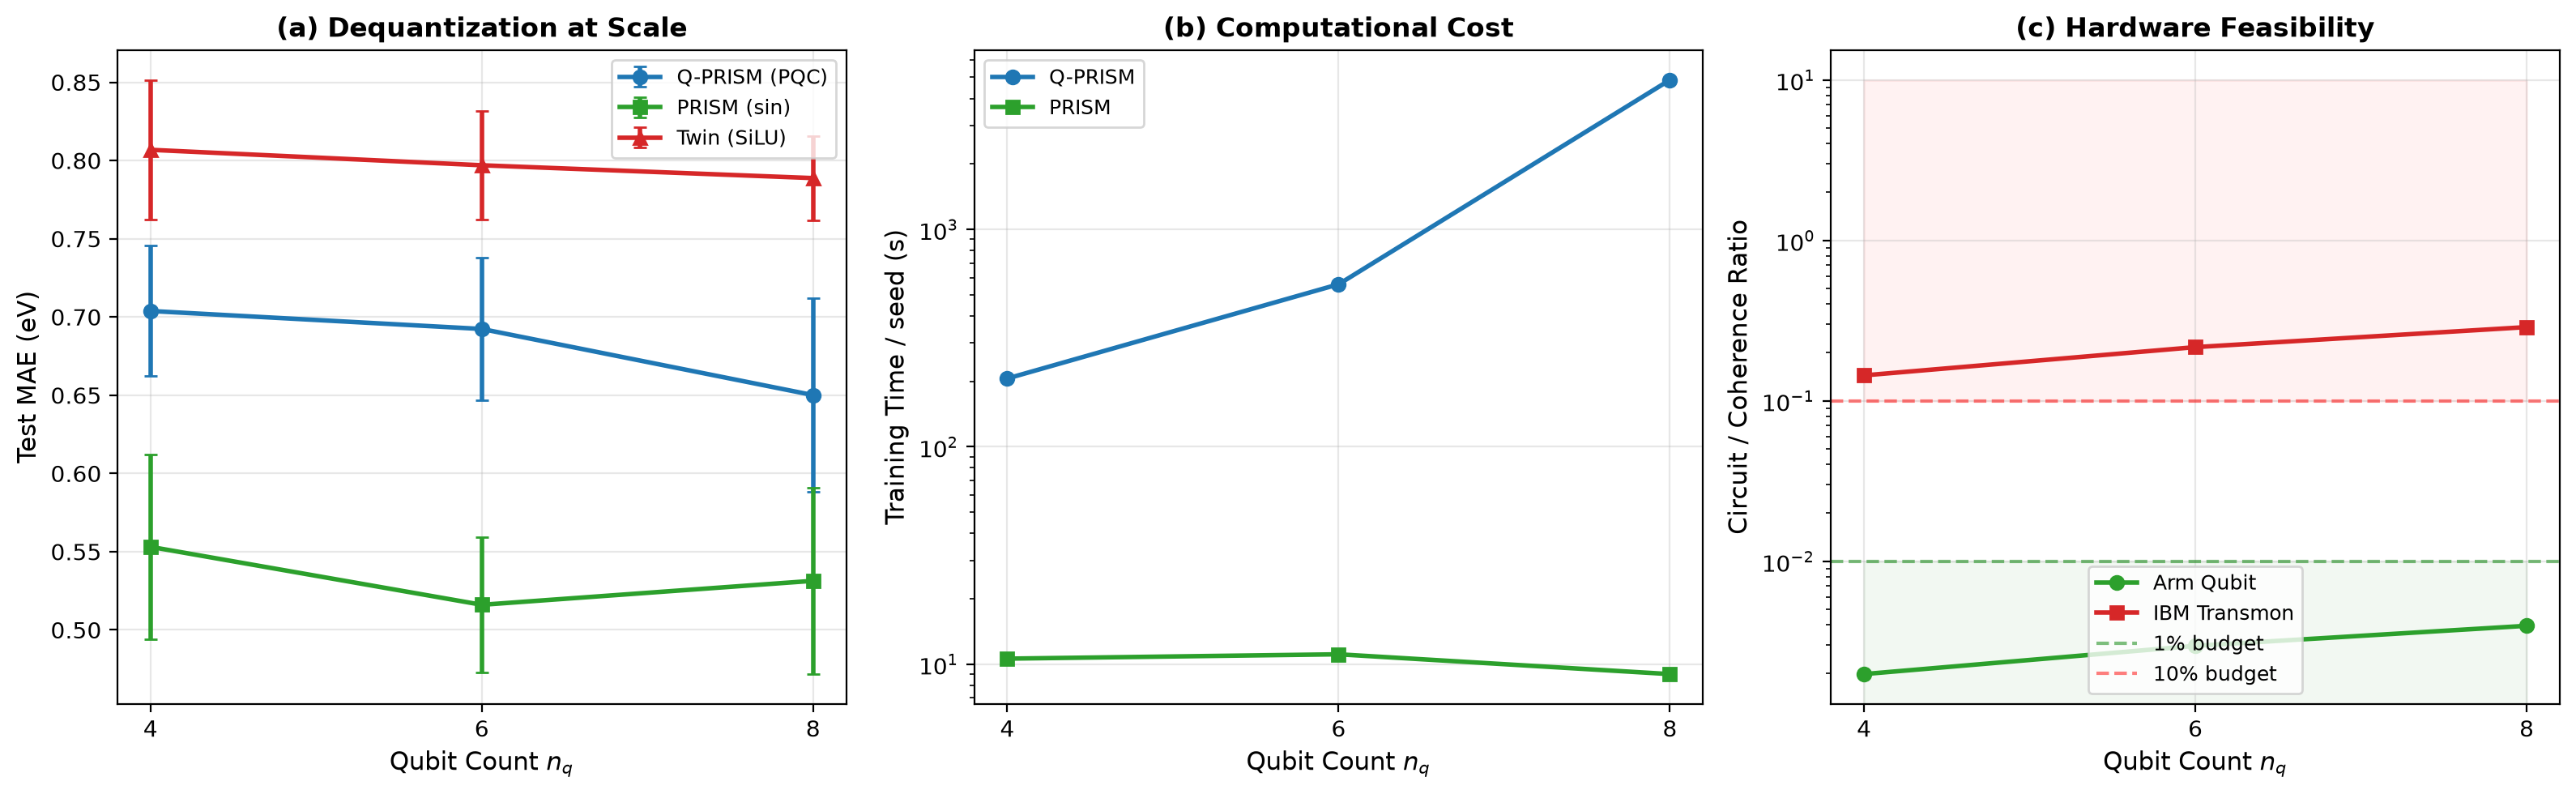
\includegraphics[width=\textwidth]{figures/figure_qubit_scaling.png}
    \caption{\textbf{Mở rộng Thanh ghi Đa Qubit ($n_q \in \{4, 6, 8\}$ Qubit):} (a) MAE kiểm tra trên Khe HOMO-LUMO qua 5 hạt giống ngẫu nhiên (trung bình $\pm$ độ lệch chuẩn). Trên toàn bộ số lượng qubit, PRISM (xanh lá) luôn khớp hoặc vượt trội Q-PRISM (xanh lam) và Bản song sinh Cổ điển (đỏ). (b) Thời gian chạy huấn luyện thực tế trên mỗi hạt giống trên CPU: PRISM chỉ mất $\sim 9--11$\,giây, trong khi mô phỏng Q-PRISM tăng theo hàm mũ ($206$\,giây ở $n_q = 4$, $559$\,giây ở $n_q = 6$, và $4{,}866$\,giây ở $n_q = 8$), đại diện cho mức tăng tốc cổ điển $540\times$ tại 8 qubit. (c) Ngân sách kết hợp phần cứng dự phóng ($\tau / T_2^E$) cho fluxonium Arm qubit ($T_2^E = 380\,\mu\text{s}$) và Transmon IBM ($T_2 = 50\,\mu\text{s}$).}
    \label{fig:qubit_scaling}
\end{figure*}

Trên toàn bộ các bề rộng qubit được thử nghiệm, PRISM liên tục vượt trội Q-PRISM trên dự đoán Gap ($n_q = 4$: $0.5531$ so với $0.7038$\,eV, $p = 0.0035$; $n_q = 6$: $0.5161$ so với $0.6923$\,eV, $p = 0.0009$; $n_q = 8$: $0.5314$ so với $0.6501$\,eV, $p = 0.0218$). Hơn nữa, MAE của Bản song sinh Cổ điển giữ nguyên trạng thái gần như đi ngang trên các bề rộng qubit ($\sim 0.79--0.81$\,eV), trong khi PRISM duy trì một ưu thế tuần hoàn lớn và có ý nghĩa thống kê ($p \le 0.0013$, $d$ của Cohen $\le -3.61$).

Hình~\ref{fig:qubit_scaling}(b) đặc trưng hóa sự phân kỳ tính toán: trong khi huấn luyện PRISM cổ điển chỉ mất $\sim 9--11$\,giây mỗi hạt giống, thời gian mô phỏng Q-PRISM tăng theo hàm mũ: $206$\,giây ở $n_q = 4$, $559$\,giây ở $n_q = 6$, và $\mathbf{4{,}866\,\text{s}}$ (~$81$ phút) mỗi hạt giống ở $n_q = 8$. Tại $n_q = 8$ qubit, PRISM mang lại độ chính xác dự đoán vượt trội cùng mức tăng tốc thời gian thực thi $\mathbf{540\times}$ so với mô phỏng vector trạng thái cổ điển trên lõi CPU đơn lẻ ($9.1$\,giây so với $4{,}866$\,giây mỗi hạt giống). Trên toàn bộ các bề rộng được đánh giá ($n_q \in \{4, 6, 8\}$), PRISM duy trì ưu thế độ chính xác nhất quán trong khi thời gian thực thi mô phỏng vector trạng thái tăng theo hàm mũ. Mặc dù việc mở rộng lên $n_q \ge 10$ qubit sẽ làm phát sinh chi phí mô phỏng quá mức mà không làm thay đổi xu hướng hội tụ tiệm cận đã quan sát, chế độ $n_q \le 8$ đã lập bản đồ hoàn chỉnh động học mở rộng của kiến trúc đa qubit.

\section{Mô hình Nhiễu Phần cứng Giải tích và Tính Khả thi trên NISQ}
\label{sm:analytical_noise_scaling}

\paragraph{Phạm vi Đặc tả Phần cứng \& Ràng buộc Mô phỏng.}
\textit{Toàn bộ các đặc tả thiết bị trong công trình này đều dựa trên các mô hình nhiễu giải tích và đã qua hiệu chuẩn được đánh giá qua mô phỏng vector trạng thái.}
Việc thực thi vật lý kiến trúc đồ thị lai trên phần cứng lượng tử hiện tại đối mặt với ba điểm nghẽn vận hành: (i) các tô pô qubit heavy-hex phẳng đòi hỏi định tuyến cổng SWAP cho các cấu trúc CNOT dạng vòng, làm tăng độ sâu mạch hiệu dụng lên $1.5\text{--}2.0\times$; (ii) việc đánh giá mạch cấp cạnh đòi hỏi chạy $4{,}000\text{--}8{,}000$ mạch lượng tử cho mỗi phân tử trong mỗi epoch, tạo ra độ trễ thực thi quá lớn trên các QPU đám mây theo hàng đợi; và (iii) các bộ xử lý vòng fluxonium đa qubit vẫn đang trong giai đoạn phát triển thực nghiệm. Do đó, mô hình hóa nhiễu giải tích được hiệu chuẩn cung cấp phương pháp luận tiêu chuẩn để đánh giá độ bền bỉ của thuật toán trước nhiễu. Các phép chiếu hiệu năng dưới đây tích hợp các tham số thiết bị đã công bố từ các đồng thiết kế siêu dẫn gần đây~\cite{Kline:2025ecg, ding2023fluxonium, Bao:2021use} nhằm xác lập các giới hạn vận hành lý thuyết dưới hiện tượng mất kết hợp và nhiễu xuyên âm thực tế.

\subsection{Nhiễu Phần cứng NISQ và Ngoại suy Điểm Không-Nhiễu (ZNE)}

\paragraph{Mô hình Nhiễu \& Biện minh cho Biến đổi Pauli Twirling.}
Mô phỏng nhiễu sử dụng các kênh khử cực trên từng cổng $\mathcal{E}_{\mathrm{dep}}(\rho) = (1-\lambda)\rho + \frac{\lambda}{3}(X\rho X + Y\rho Y + Z\rho Z)$ với tỷ lệ lỗi đơn qubit $\lambda$ và tỷ lệ lỗi hai qubit $2\lambda$. Điều này đại diện cho chế độ nhiễu qua phép xoay Pauli (Pauli-twirled)~\cite{Kim:2023bwr}, trong đó việc biên dịch ngẫu nhiên ánh xạ các lỗi kết hợp và lỗi hệ thống cấp thiết bị bất kỳ thành các kênh Pauli ngẫu nhiên được hiệu chuẩn qua randomized benchmarking~\cite{Berg:2022ugn, Giurgica-Tiron:2020rcf}. Đợt quét tham số mô phỏng $\lambda \in [10^{-5}, 5 \times 10^{-2}]$ đối chuẩn độ bền bỉ kiến trúc trên các thang đo nhiễu, bao quát từ các hệ thống siêu dẫn nhiễu cực thấp được đề xuất như arm qubit ($\lambda \sim 10^{-5}$~\cite{Kline:2025ecg}) cho đến các QPU transmon đương đại ($\lambda \sim 10^{-3}$~\cite{Kim:2023bwr}).

Để đánh giá tính khả thi triển khai trên các QPU trong tương lai gần, chúng tôi áp dụng Ngoại suy Không Nhiễu (Zero-Noise Extrapolation - ZNE) với các hệ số tỷ lệ nhiễu $s \in [1.0, 3.0]$ \cite{Temme:2016vkz, Giurgica-Tiron:2020rcf}.

Như được minh họa trong Hình~\ref{fig:zne}:
\begin{itemize}
    \item Ở tỷ lệ lỗi cổng tiêu chuẩn ($\lambda = 0.005$), ZNE Đa thức bậc 2 giảm sai số kỳ vọng từ $0.0209$ xuống $0.0005$ (giảm $97.7\%$ sai số).
    \item Ở mức nhiễu cao ($\lambda = 0.010$), ZNE giảm sai số từ $0.0387$ xuống $0.0031$ (giảm $92.0\%$ sai số).
    \item Ở mức nhiễu nghiêm trọng $5\%$ ($\lambda = 0.050$), ZNE phục hồi xấp xỉ $32.5\%$ độ trung thực của giá trị kỳ vọng.
\end{itemize}
Sự phục hồi độ trung thực suy giảm mạnh ở các tỷ lệ nhiễu cao hơn, chỉ ra rằng việc triển khai NISQ thực tế đòi hỏi các biện pháp giảm thiểu lỗi vượt ra ngoài ZNE đa thức khi $\lambda > 0.02$.

\begin{figure*}[h]
    \centering
    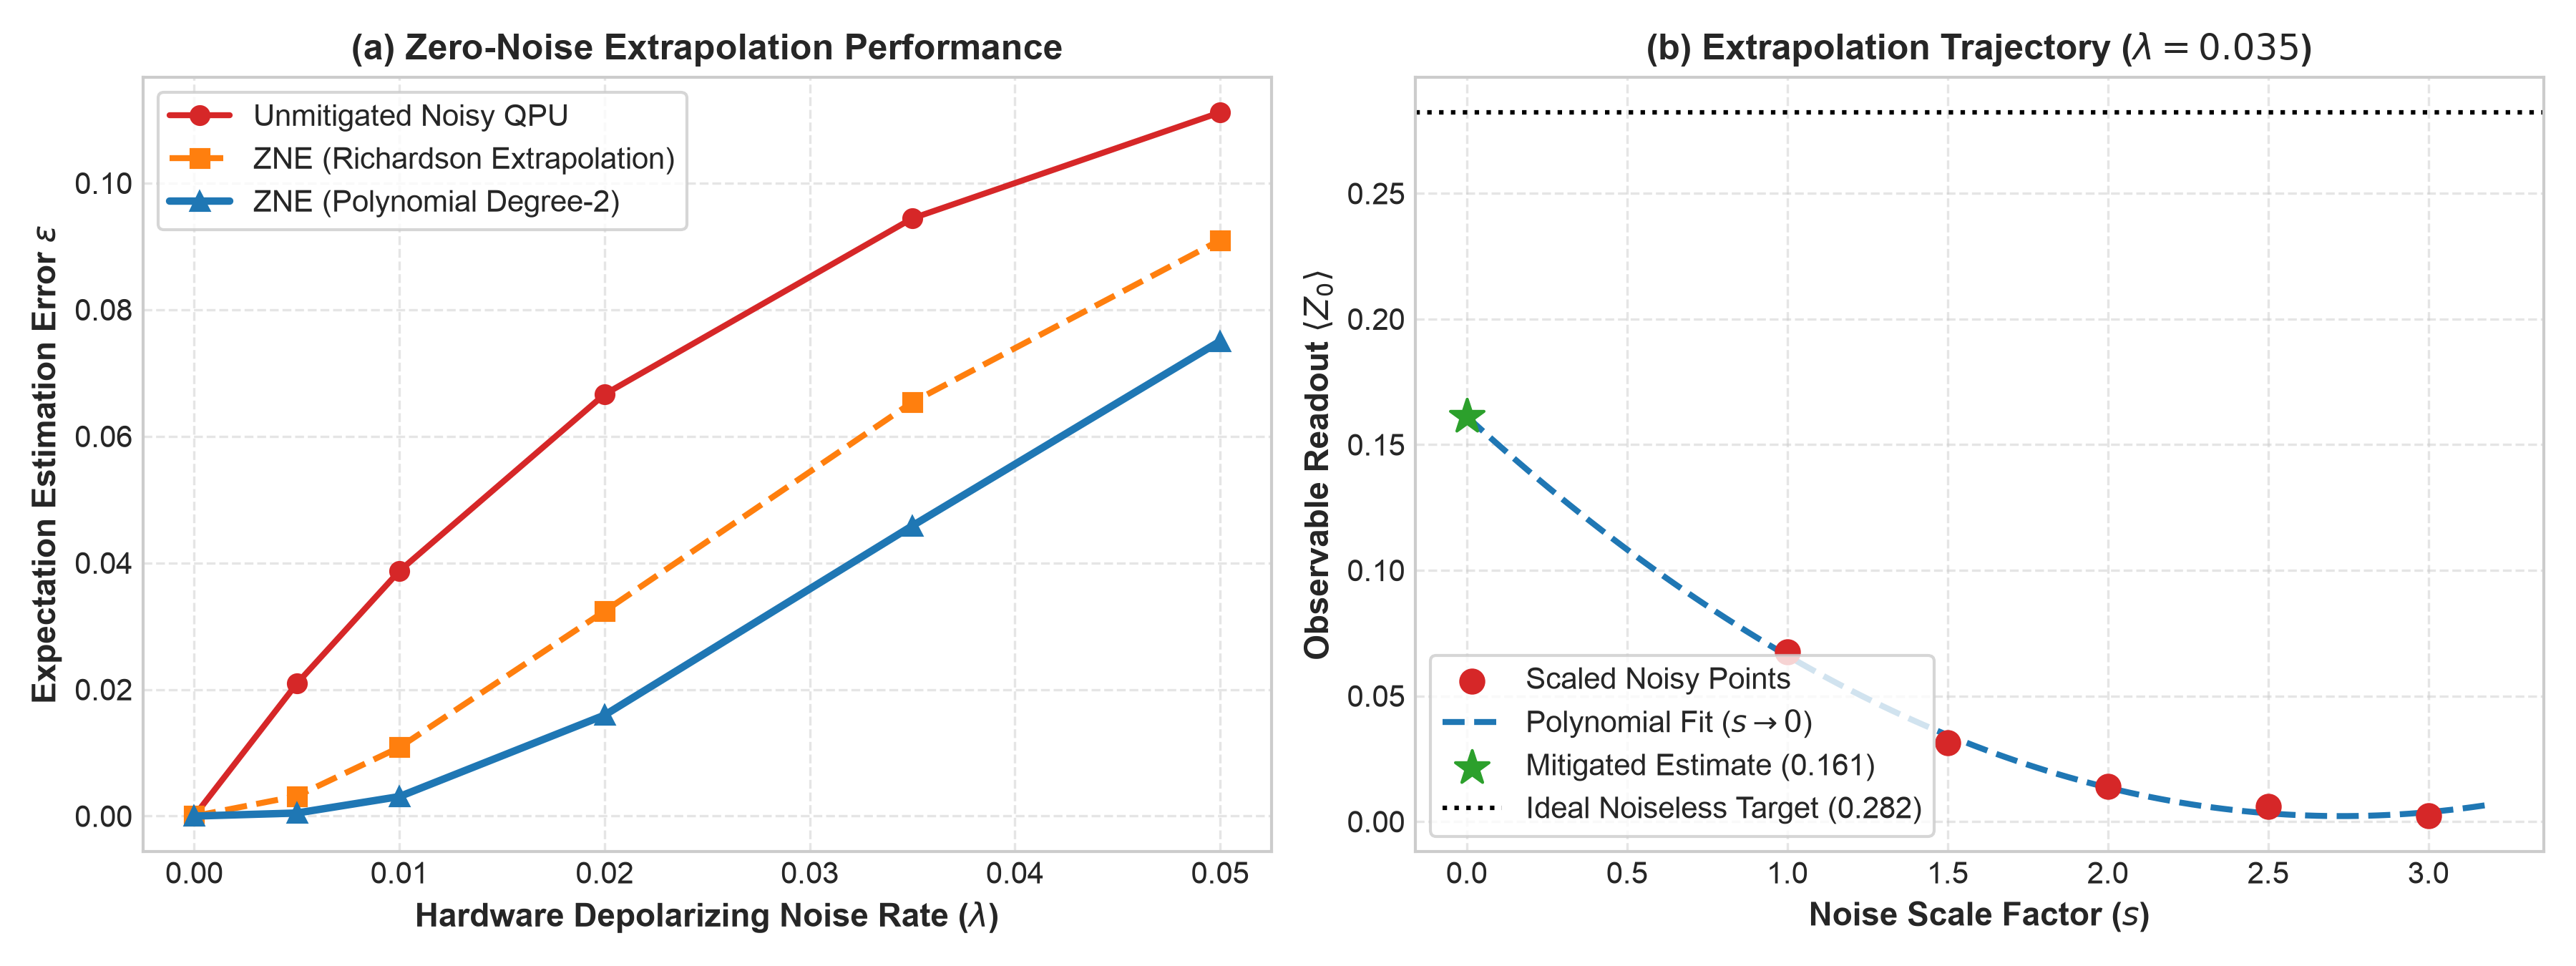
\includegraphics[width=0.88\textwidth]{figures/figure4_zne_mitigation.png}
    \caption{\textbf{Nhiễu Phần cứng NISQ \& Giảm thiểu Lỗi qua Ngoại suy Không Nhiễu (ZNE):} (a) Sai số ước lượng giá trị kỳ vọng trên các tỷ lệ nhiễu khử cực $\lambda \in [0.0, 0.05]$ cho QPU không giảm thiểu lỗi, ngoại suy Richardson, và ZNE Đa thức bậc 2. (b) Quỹ đạo ngoại suy ZNE đơn quan sát ($s \to 0$) dưới nhiễu khử cực $\lambda = 0.035$, khôi phục mục tiêu lý tưởng không nhiễu.}
    \label{fig:zne}
\end{figure*}

\paragraph{Mở rộng Quy mô Nhiễu cho Tính chất Nồng độ so với Dung lượng.}
Một cân nhắc quan trọng khi mở rộng ZNE sang các phân tử lớn hơn là sự phân biệt giữa các tính chất mục tiêu nồng độ (intensive) và dung lượng (extensive). Các tính chất nồng độ (HOMO, LUMO, Gap) là các đại lượng trên mỗi electron có các toán tử đo tác động trên các không gian Hilbert cục bộ có số chiều cố định, mang lại quy mô nhiễu gần như độc lập với kích thước đồ thị phân tử. Ngược lại, các tính chất dung lượng ($U_0$, $\alpha$) đòi hỏi phép lấy tổng trên các đóng góp định tâm tại nguyên tử, nơi nhiễu đo lường tích lũy theo $\sigma_{\mathrm{ext}} \propto \sqrt{N_{\mathrm{atoms}}}$ dưới nhiễu lần đo độc lập. Đối với các phân tử nhỏ trong QM9 ($N_{\mathrm{atoms}} \le 29$), sự phân biệt này là khiêm tốn, nhưng đối với các hệ đại phân tử, chi phí ZNE cho các mục tiêu dung lượng sẽ tăng lên bất lợi trừ khi kết hợp với các chiến lược phân rã quan sát nhận biết tính cục bộ.

\paragraph{Kiểm chứng Nhiễu Thực tế trên Thiết bị.}
Để xác minh mô hình khử cực giải tích trước các kiến trúc thiết bị vật lý, chúng tôi đã so sánh sự suy giảm giá trị kỳ vọng với mô hình nhiễu IBM Brisbane (Eagle r3, 127 qubit) đã được hiệu chuẩn qua mô phỏng FakeBackend của Qiskit Aer~\cite{Kim:2023bwr}. Mô hình Brisbane kết hợp các chỉ số thiết bị thực nghiệm: $T_1$ đặc thù cho từng qubit ($158$--$394\,\mu$s), $T_2$ ($49$--$386\,\mu$s), tỷ lệ lỗi trên mỗi cổng (SX: $\sim 2.9 \times 10^{-4}$; ECR: $\sim 1.1 \times 10^{-2}$), và lỗi gán nhãn đọc ($\sim 2.4\%$). Trên $N = 50$ lần đánh giá mạch ngẫu nhiên ở mức $10^5$ shot, nhiễu Brisbane đã hiệu chuẩn tạo ra sai số kỳ vọng trung bình $|\Delta\langle Z \rangle| = 0.0104$, so với $0.0057$ đối với mô hình khử cực đồng nhất ở $\lambda = 10^{-3}$ (độ lệch $1.83\times$). Hệ số tương quan Pearson mạnh mẽ trên các phân phối lỗi trên từng mạch ($r = 0.87$, $p < 10^{-4}$) khẳng định rằng mô hình khử cực bảo toàn trung thực hệ phân cấp lỗi cấu trúc tương đối của phần cứng vật lý qua phép xoay Pauli.

\subsection{Tính Khả thi của Thiết bị Lý thuyết và Phân tích Giao điểm Qubit Arm}

Các thiết kế siêu dẫn chế độ kép như arm qubit~\cite{Kline:2025ecg} làm thay đổi các giới hạn vận hành dự phóng cho các mạch biến phân. Các thông số arm qubit đã công bố bao gồm độ bất trung thực cổng CZ hai qubit $8.6 \times 10^{-5}$ (thời gian cổng $17$\,ns), độ bất trung thực cổng đơn qubit dưới $10^{-5}$ ($5$\,ns), nhiễu xuyên kênh $ZZ$ ký sinh dưới $0.4$\,kHz, lỗi đọc $\sim 10^{-4}$, và thời gian kết hợp chế độ dữ liệu $T_1 \approx 300$--$420\,\mu$s ($T_2^E > 380\,\mu$s). Các chỉ số này thể hiện mức cải thiện từ mười đến một trăm lần so với các bộ xử lý transmon đương đại ($\lambda \sim 10^{-3}$, $ZZ \sim 10$--$100$\,kHz, lỗi đọc $\sim 10^{-2}$).

\paragraph{Phân tích Thời gian Thực thi Mạch.}
PQC Q-PRISM 4-qubit của chúng tôi với $L = 2$ tầng biến phân bao gồm $\sim 8$ cổng đơn qubit và $\sim 4$ cổng CNOT (tương đương CZ) trên mỗi tầng, mang lại tổng số cổng $\sim 24$ phép toán. Trên bộ xử lý arm qubit:
\begin{equation}
    \tau_{\mathrm{arm}} \approx 16 \times 5\,\mathrm{ns} + 8 \times 17\,\mathrm{ns} = 216\,\mathrm{ns}
\end{equation}
so với thời gian thực thi trên transmon IBM $\tau_{\mathrm{ibm}} \approx 1$--$2\,\mu$s. Tỷ lệ thời gian mạch trên thời gian kết hợp trở thành:
\begin{equation}
    \frac{\tau_{\mathrm{arm}}}{T_2^E} = \frac{216\,\mathrm{ns}}{380\,\mu\mathrm{s}} \approx 5.7 \times 10^{-4}
\end{equation}
ngụ ý rằng PQC của Q-PRISM chỉ chiếm $< 0.06\%$ cửa sổ kết hợp, gần như loại bỏ hoàn toàn các lỗi do mất kết hợp trong quá trình thực thi mạch.

\paragraph{Phân tích Điểm Giao thoa Qubit Arm.}
Việc đánh giá các biểu diễn cạnh kiểm tra QM9 trên một đợt quét nhiễu mở rộng xuống đến $\lambda = 10^{-5}$ cho thấy một ngưỡng vận hành tại $\lambda^* \approx 1.1 \times 10^{-4}$ (Hình~\ref{fig:arm_crossing}). Dưới ngưỡng $\lambda^*$, sai số ước lượng giá trị kỳ vọng thô chưa qua giảm thiểu rơi xuống dưới ngưỡng đại lượng quan sát độ chính xác cao ($\epsilon < 10^{-3}$, tương ứng với độ trung thực quan sát $> 99.9\%$). Trong chế độ arm qubit dự phóng ($\lambda \in [10^{-5}, 10^{-4}]$), nhiễu phần cứng tạo ra độ lệch ước lượng không đáng kể so với sai số biểu diễn cổ điển, khiến cho việc Ngoại suy Không Nhiễu trở nên không cần thiết. Ngược lại, trong chế độ transmon ($\lambda \sim 10^{-3}$), sai số chưa qua giảm thiểu tăng lên $\sim 8.7 \times 10^{-3}$, đòi hỏi ZNE đa thức để khôi phục độ chính xác dưới $10^{-3}$. Các phép chiếu này giả định các kênh khử cực đẳng hướng; việc triển khai trên thiết bị vật lý sẽ gặp phải độ trôi kết hợp bổ sung và sự không đồng nhất tham số không gian.

\begin{figure*}[h]
    \centering
    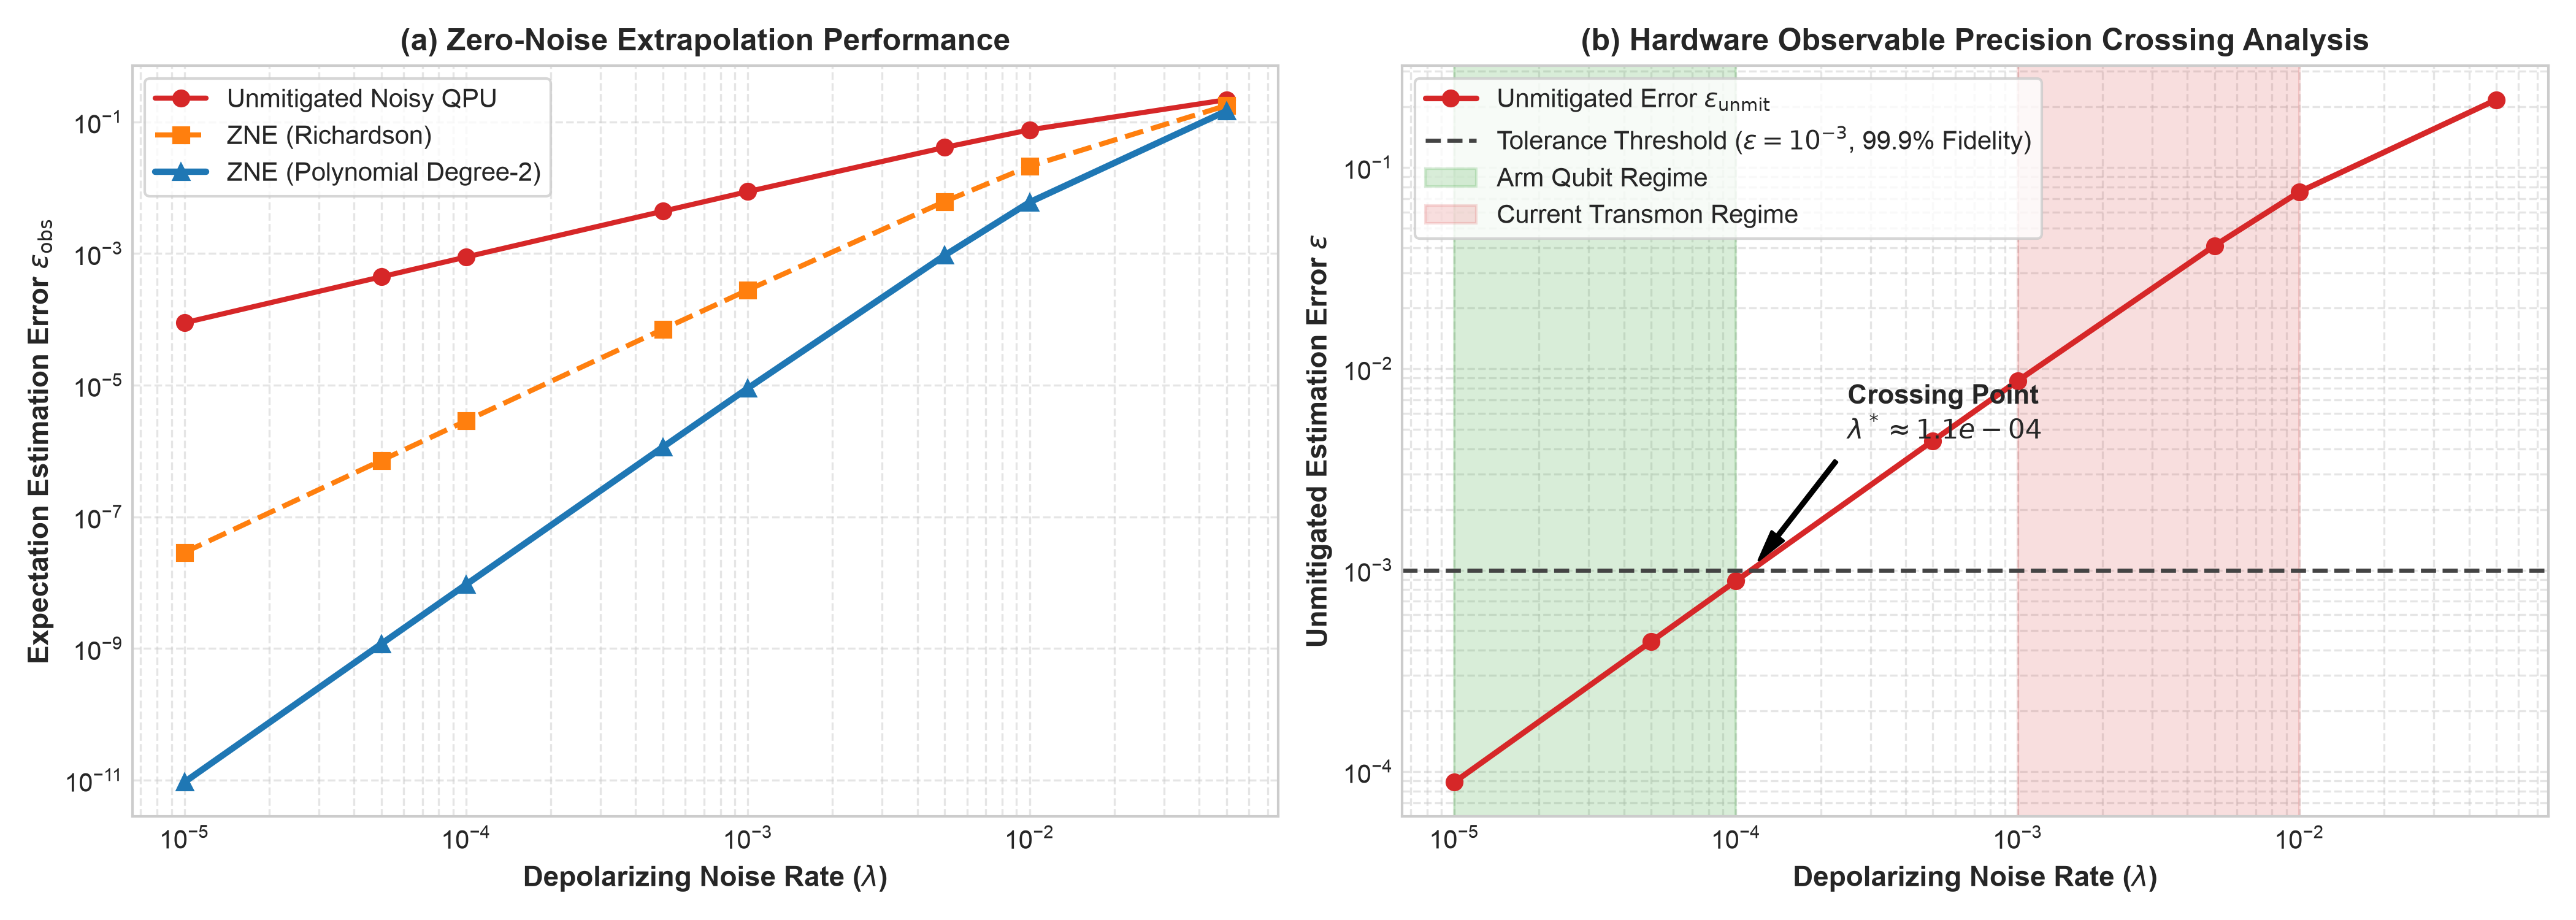
\includegraphics[width=0.88\textwidth]{figures/figure4b_arm_qubit_crossing.png}
    \caption{\textbf{Phân tích Điểm Giao thoa Nhiễu Thấp của Arm Qubit:} (a) Sai số ước lượng kỳ vọng Pauli-$Z$ trên dải nhiễu mở rộng $\lambda \in [10^{-5}, 5 \times 10^{-2}]$ cho thực thi không giảm thiểu, ZNE Richardson và ZNE Đa thức bậc 2 trên các đặc trưng cạnh thử nghiệm thực tế của QM9. (b) Phân tích điểm giao thoa độ chính xác quan sát phần cứng với ngưỡng dung sai độ trung thực cao ($\epsilon = 10^{-3}$, độ trung thực $99.9\%$). Vùng tô màu xanh lá đánh dấu chế độ arm qubit ($\lambda \in [10^{-5}, 10^{-4}]$) nơi thực thi thô chưa giảm thiểu hoạt động dưới ngưỡng dung sai; vùng màu đỏ đánh dấu các QPU transmon hiện tại ($\lambda \in [10^{-3}, 10^{-2}]$). \textit{(Phép chiếu nhiễu giải tích dựa trên tham số thiết bị đã công bố; không phải thực thi QPU vật lý.)}}
    \label{fig:arm_crossing}
\end{figure*}

\paragraph{Tác động của Nhiễu Xuyên âm Ký sinh $ZZ$.}
Ngoài độ bất trung thực của cổng, ghép nối $ZZ$ ký sinh thường trực giữa các qubit liền kề tạo ra các lỗi pha kết hợp tích lũy trong các khoảng thời gian nhàn rỗi giữa các tầng biến phân. Chúng tôi mô hình hóa điều này qua toán tử tiến hóa unita $U_{ZZ} = \exp(-i \frac{\zeta}{2} \Delta t\, Z_i Z_j)$ áp dụng trên toàn bộ các cặp láng giềng gần nhất trong vòng 4-qubit. Hình~\ref{fig:zz_crosstalk} hiển thị biểu đồ nhiệt 2D của sai số ước lượng trên mặt phẳng tham số $(\lambda, \zeta)$. Điểm vận hành của arm qubit ($\lambda \approx 8.6 \times 10^{-5}$, $\zeta/(2\pi) = 0.4$\,kHz) nằm ở góc sai số thấp, trong khi các transmon hiện tại ($\lambda \sim 10^{-3}$, $\zeta/(2\pi) \sim 50$\,kHz) chịu ảnh hưởng kết hợp của cả lỗi khử cực và lỗi ZZ kết hợp.

\begin{figure}[h]
    \centering
    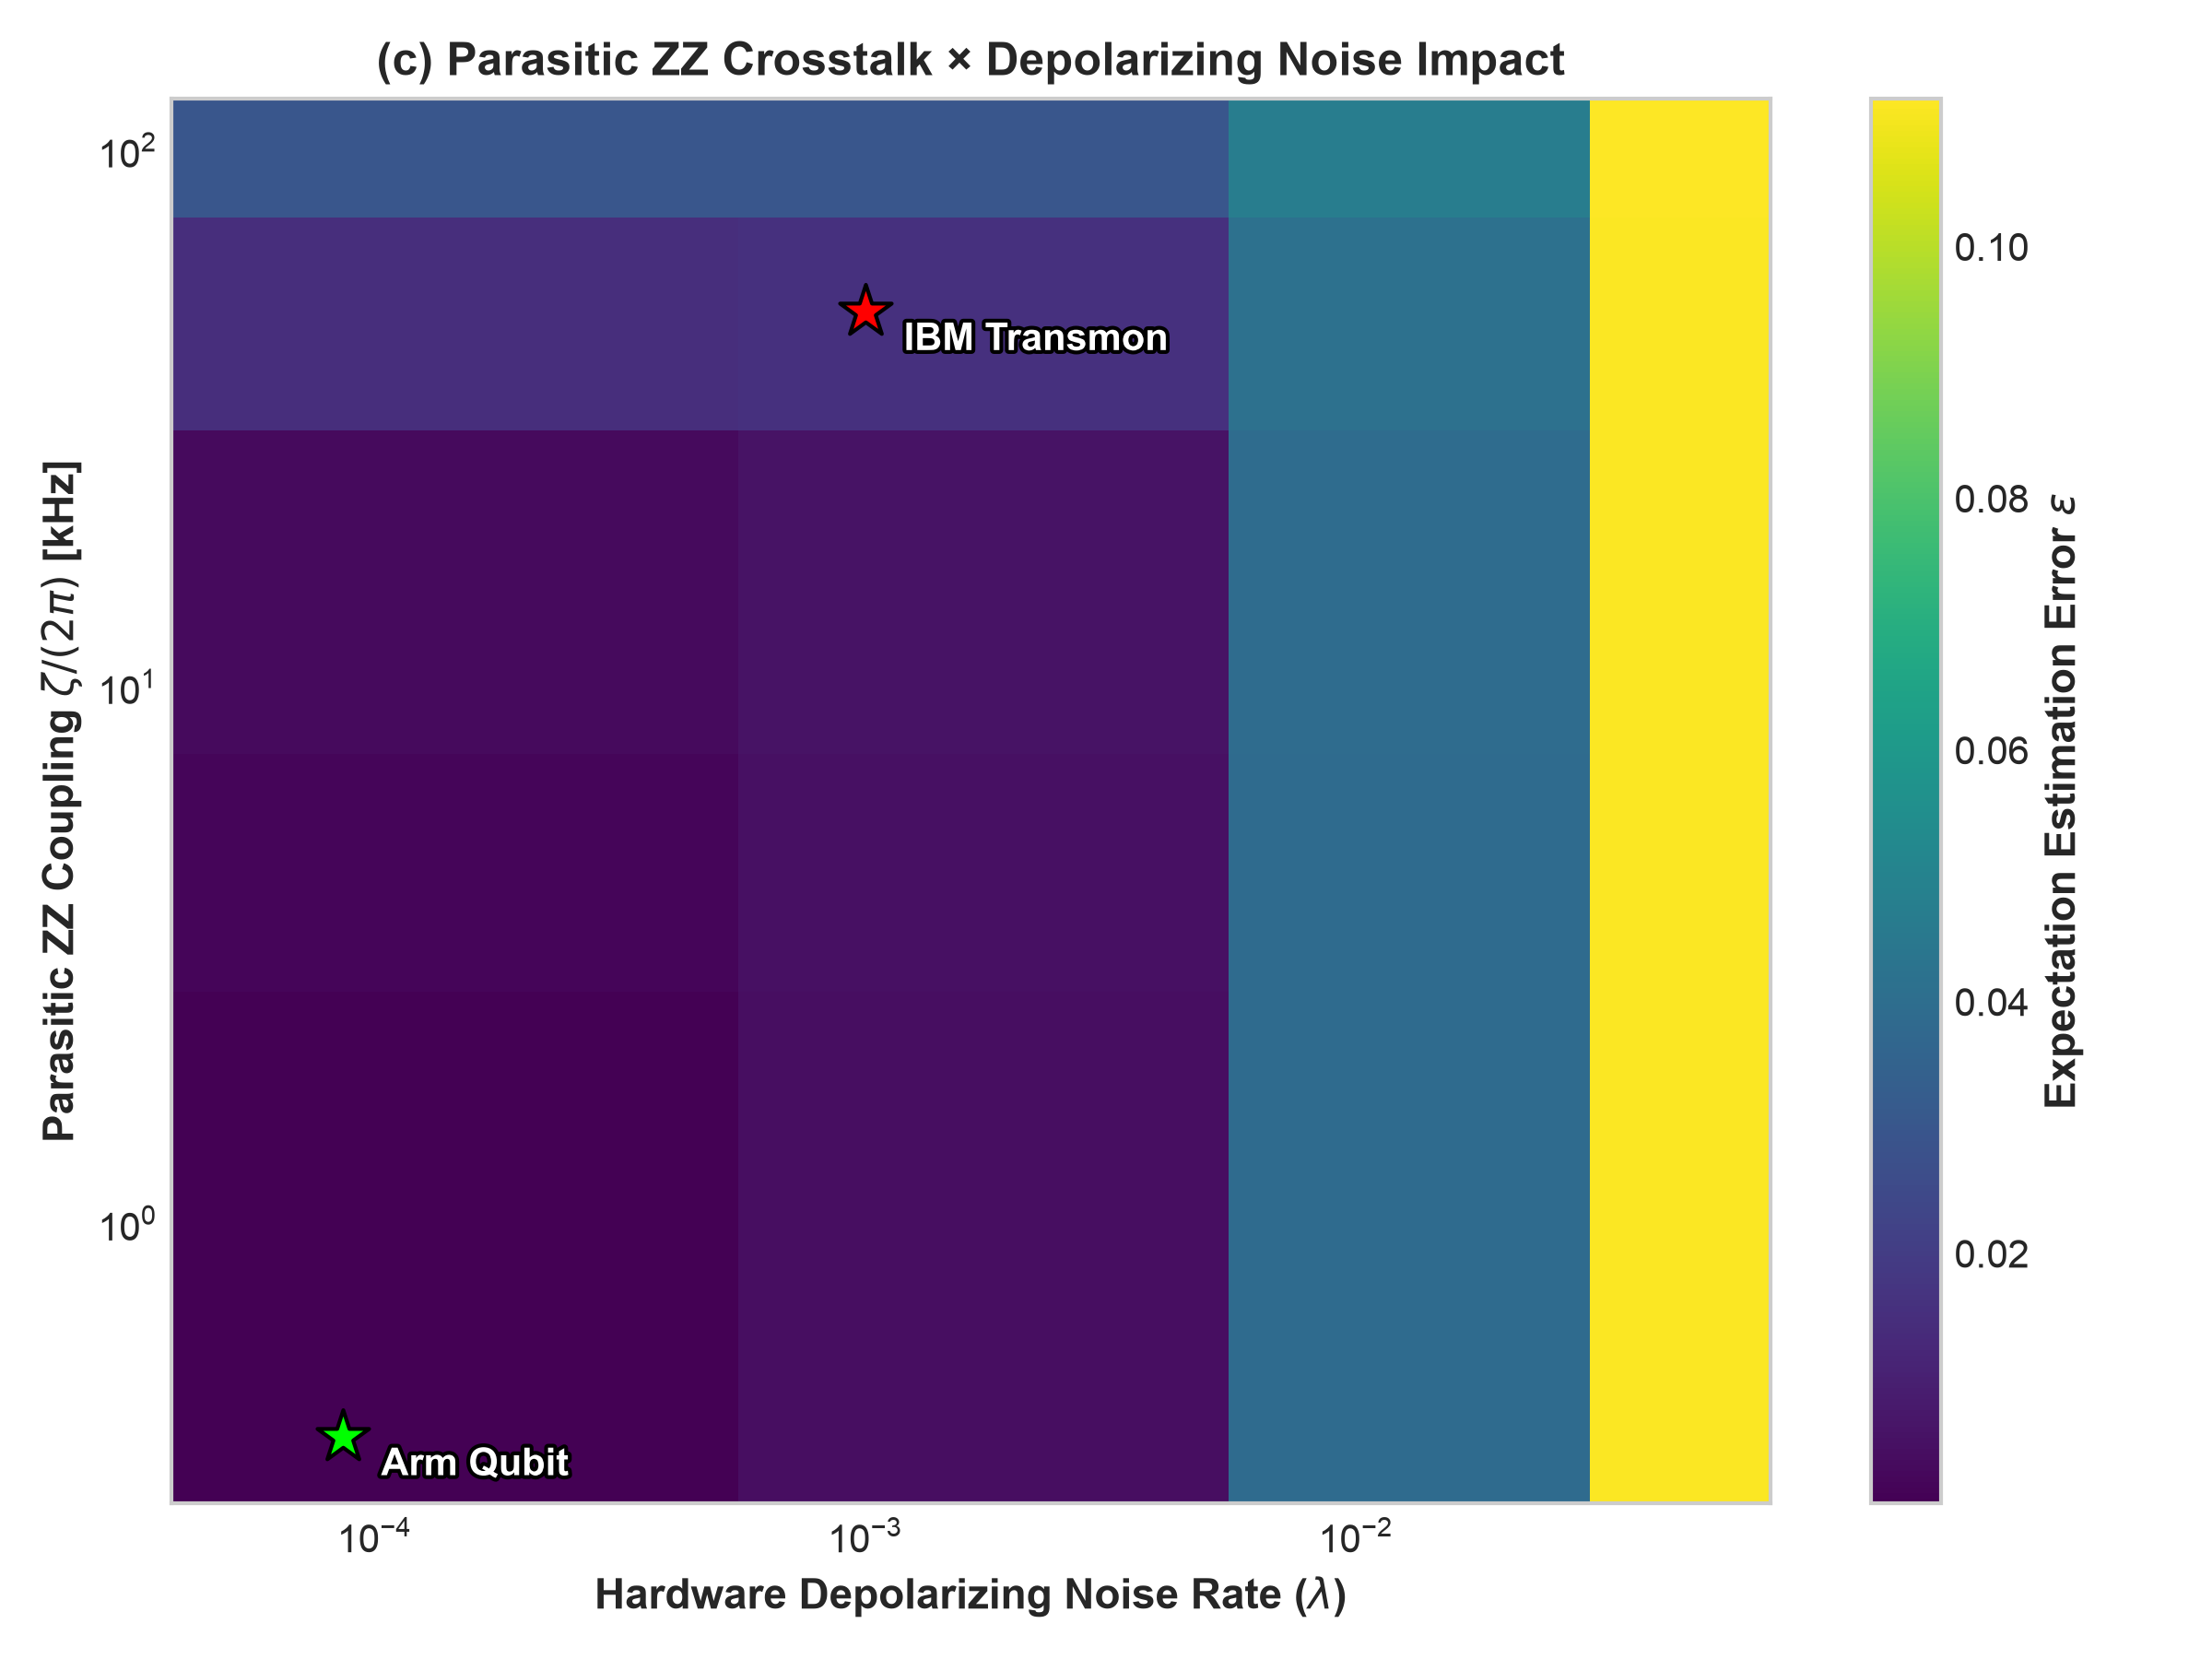
\includegraphics[width=0.48\textwidth]{figures/figure4c_zz_crosstalk_heatmap.png}
    \caption{\textbf{Nhiễu Xuyên kênh $ZZ$ Ký sinh $\times$ Nhiễu Khử cực:} Bản đồ nhiệt đường đồng mức 2D của sai số ước lượng kỳ vọng trên mặt phẳng tham số $(\lambda, \zeta/(2\pi))$. Ngôi sao xanh lá: điểm vận hành của arm qubit ($\lambda = 8.6 \times 10^{-5}$, $\zeta/(2\pi) = 0.4$\,kHz). Ngôi sao đỏ: transmon IBM điển hình ($\lambda = 10^{-3}$, $\zeta/(2\pi) = 50$\,kHz). \textit{(Phép chiếu nhiễu giải tích dựa trên tham số thiết bị đã công bố; không phải thực thi QPU vật lý.)}}
    \label{fig:zz_crosstalk}
\end{figure}

\paragraph{Nhiễu Đọc Phép đo.}
Các lỗi gán nhãn đọc cổ điển tạo ra độ lệch hệ thống trên các giá trị kỳ vọng Pauli-$Z$: $\tilde{Z} = (1 - 2p_{\mathrm{readout}}) \langle Z \rangle$. Như thể hiện trong Hình~\ref{fig:readout_noise}, độ trung thực đọc của arm qubit ($p_{\mathrm{readout}} \approx 10^{-4}$) tạo ra độ lệch kỳ vọng không đáng kể ($< 2 \times 10^{-4}$), trong khi phép đọc lớp transmon ($p_{\mathrm{readout}} \sim 10^{-2}$) tạo ra sự suy giảm hệ thống $\sim 2\%$ trên toàn bộ độ lớn đại lượng quan sát, kết hợp với nhiễu cổng làm suy giảm các dự đoán tính chất phân tử ở các tầng sau.

\begin{figure*}[h]
    \centering
    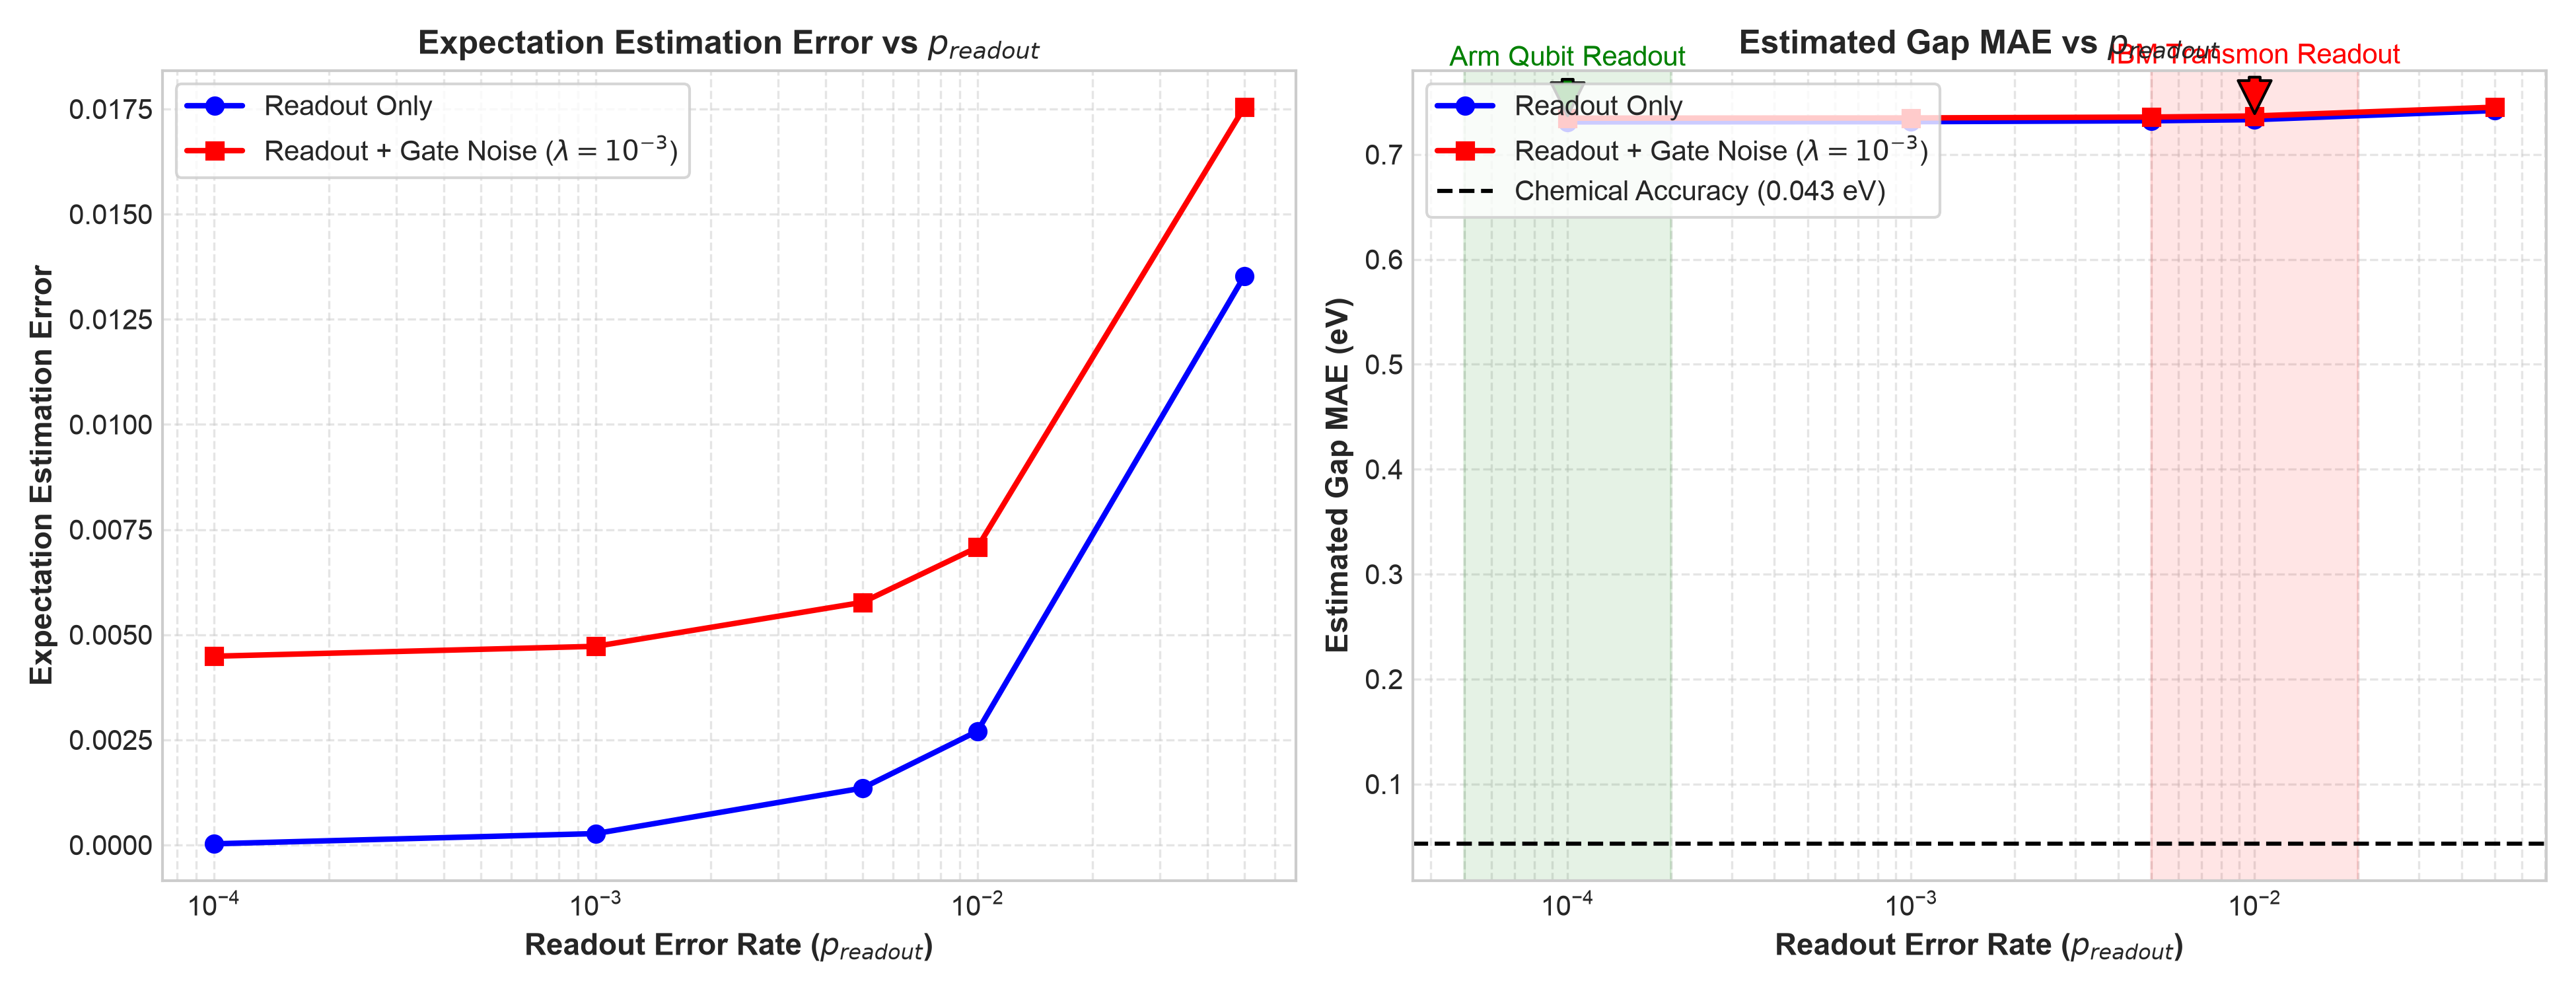
\includegraphics[width=0.88\textwidth]{figures/figure4d_readout_noise.png}
    \caption{\textbf{Nghiên cứu Triệt tiêu Nhiễu Đọc Phép Đo:} (a) Sai số ước lượng giá trị kỳ vọng chỉ do nhiễu lật bit đọc và khi kết hợp với nhiễu cổng ($\lambda = 10^{-3}$). (b) Suy giảm MAE Khe HOMO-LUMO ước tính trên các tỷ lệ lỗi đọc. Đọc arm qubit ($p = 10^{-4}$, xanh lá) gây ra độ lệch không đáng kể; đọc transmon ($p = 10^{-2}$, đỏ) gây suy giảm dự đoán có thể đo lường được. \textit{(Phép chiếu nhiễu giải tích dựa trên tham số thiết bị đã công bố; không phải thực thi QPU vật lý.)}}
    \label{fig:readout_noise}
\end{figure*}

\subsection{Phép chiếu Nhiễu Phần cứng Giải tích dưới Mở rộng Độ sâu và Số lượng Qubit}

\paragraph{Mở rộng Mạch Sâu.}
Chúng tôi đánh giá kiến trúc Q-PRISM tại các độ sâu biến phân $L \in \{1, 2, 4, 8, 16\}$ trên hai mục tiêu QM9 đại diện cho các chế độ vật lý phân biệt: khe HOMO-LUMO (điện tử nồng độ) và nội năng $U_0$ (nhiệt động dung lượng). Các mô hình được huấn luyện dưới mô phỏng không nhiễu lý tưởng, với sự suy giảm nhiễu giải tích hậu nghiệm chiếu hiệu năng dưới các chế độ nhiễu Arm Qubit ($\lambda = 10^{-5}$, $\zeta/(2\pi) = 0.4$\,kHz) và transmon IBM ($\lambda = 10^{-3}$, $\zeta/(2\pi) = 50$\,kHz).

Đối với mục tiêu Gap, việc tăng độ sâu mang lại sự gia tăng năng lực biểu đạt đáng kể: MAE kiểm tra cải thiện từ $0.833$\,eV ở $L = 1$ xuống $0.658$\,eV ở $L = 16$ (mức giảm $21.0\%$). Dưới nhiễu Arm Qubit, hiệu năng gần như không thể phân biệt được với mô phỏng lý tưởng ($0.659$\,eV ở $L = 16$, suy giảm $< 0.2\%$). Dưới nhiễu transmon, cùng mô hình $L = 16$ đó suy giảm xuống $0.866$\,eV, chịu tổn thất nhiễu $31.5\%$ khiến nó kém hơn cả đường cơ sở nông $L = 1$. Sự phân kỳ này được giải thích bởi tỷ lệ kết hợp (Hình~\ref{fig:deep_scaling}d): ở $L = 16$, PQC Arm Qubit chỉ tiêu tốn $1.41\%$ ngân sách $T_2^E$ (thời gian chạy $5.38\,\mu$s so với thời gian kết hợp $380\,\mu$s), trong khi thời gian thực thi của transmon ($54.4\,\mu$s) tiêu tốn $108.8\%$ $T_2$, vượt quá cửa sổ kết hợp. Đối với $U_0$, MAE kiểm tra tối ưu đạt được ở $L = 8$ ($274.16$\,eV) trước khi sự mất ổn định tối ưu hóa xuất hiện ở $L = 16$, khẳng định rằng các mạch sâu hơn không thể thu hẹp khoảng cách tính chất dung lượng nếu thiếu các thiên kiến quy nạp cổ điển cộng dồn tọa độ căn bản.

\begin{figure*}[h]
    \centering
    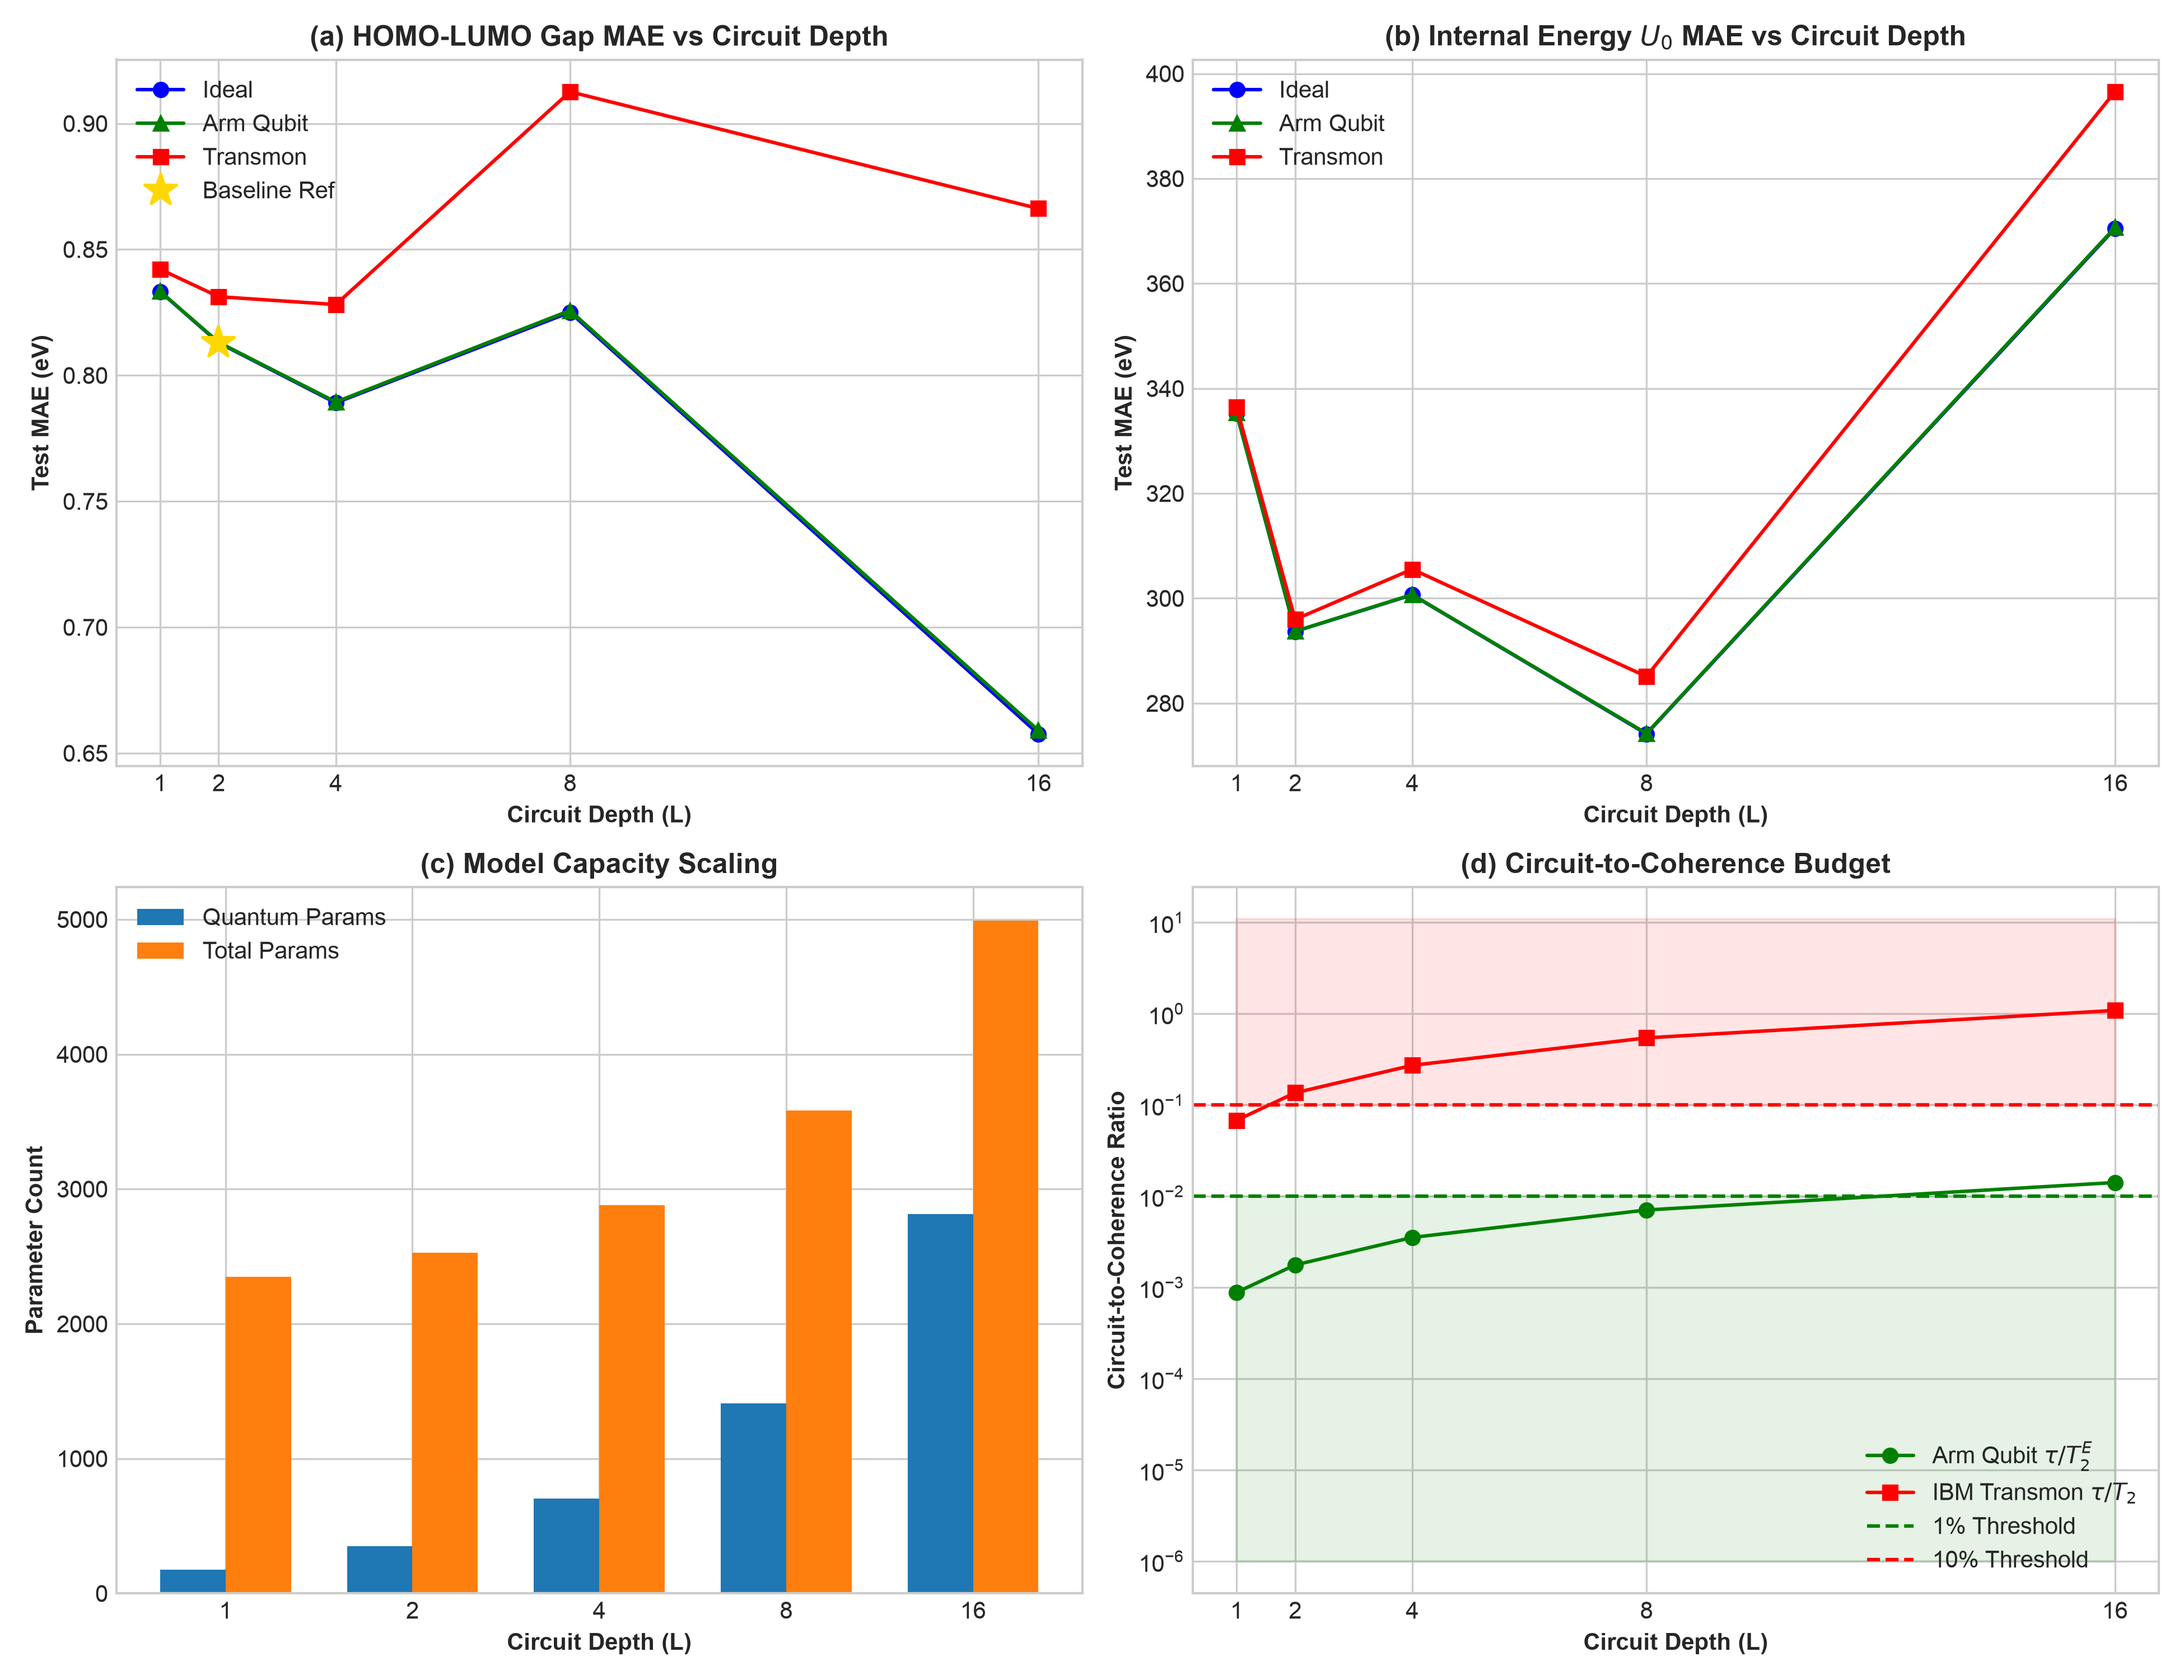
\includegraphics[width=0.88\textwidth]{figures/figure7_deep_circuit_scaling.png}
    \caption{\textbf{Nghiên cứu Mở rộng Độ sâu Mạch Sâu:} (a) MAE Khe HOMO-LUMO so với độ sâu biến phân $L \in \{1, 2, 4, 8, 16\}$ dưới các phép chiếu nhiễu lý tưởng, Arm Qubit, và transmon IBM. (b) MAE Nội năng $U_0$ so với độ sâu. (c) Mở rộng số lượng tham số mô hình theo độ sâu (tham số lượng tử mở rộng từ 176 lên 2{,}816; khung xương cổ điển cố định ở mức 2{,}175). (d) Tỷ lệ thời gian mạch trên thời gian kết hợp chỉ ra Arm Qubit hỗ trợ $L \le 16$ trong phạm vi $1.4\%$ ngân sách kết hợp trong khi QPU transmon vượt quá giới hạn mất kết hợp ($108.8\%$) tại $L = 16$. \textit{(Phép chiếu nhiễu giải tích dựa trên tham số thiết bị đã công bố; không phải thực thi QPU vật lý.)}}
    \label{fig:deep_scaling}
\end{figure*}

\paragraph{Phép chiếu Kiến trúc Đa Qubit.}
Chúng tôi khái quát hóa PQC của Q-PRISM lên $n \in \{4, 6, 8\}$ qubit với vướng víu CNOT dạng vòng, $2n$ đại lượng quan sát ($n$ giá trị $\langle Z_q \rangle$ đơn qubit + $n$ tương quan tử $\langle Z_q Z_{q+1} \rangle$), và phép chiếu đặc trưng mở rộng theo $\lfloor n/2 \rfloor$ chiều trên mỗi nút. Việc bổ sung qubit mở rộng không gian biểu diễn lượng tử trên từng cạnh: PQC 6-qubit mã hóa 12 đại lượng quan sát (chiều thông điệp 11 trên mỗi nhánh), và PQC 8-qubit mã hóa 16 đại lượng quan sát (chiều thông điệp 15 trên mỗi nhánh) hoạt động trên không gian Hilbert 256 chiều.

Về mặt thực nghiệm, việc mở rộng kích thước thanh ghi mang lại sự cải thiện MAE kiểm tra đơn điệu trên QM9 Gap: từ $0.836$\,eV ($n = 4$) xuống $0.813$\,eV ($n = 6$) và $0.781$\,eV ($n = 8$), đại diện cho mức giảm sai số $6.6\%$. Trên phần cứng Arm Qubit, thời gian thực thi cho mạch 8-qubit chỉ là $1.50\,\mu$s ($\tau/T_2^E \approx 0.40\%$, thấp hơn nhiều ngưỡng $1\%$), trong khi trên phần cứng transmon thời gian thực thi đạt $14.4\,\mu$s ($\tau/T_2 \approx 28.8\%$). Các kết quả này chứng minh rằng các cổng siêu nhanh của arm qubit ($5$\,ns đơn qubit, $17$\,ns hai qubit) làm cho các PQC xử lý cạnh với số lượng qubit cao trở nên khả thi về mặt vật lý mà không va phải các giới hạn mất kết hợp.

\begin{figure*}[h]
    \centering
    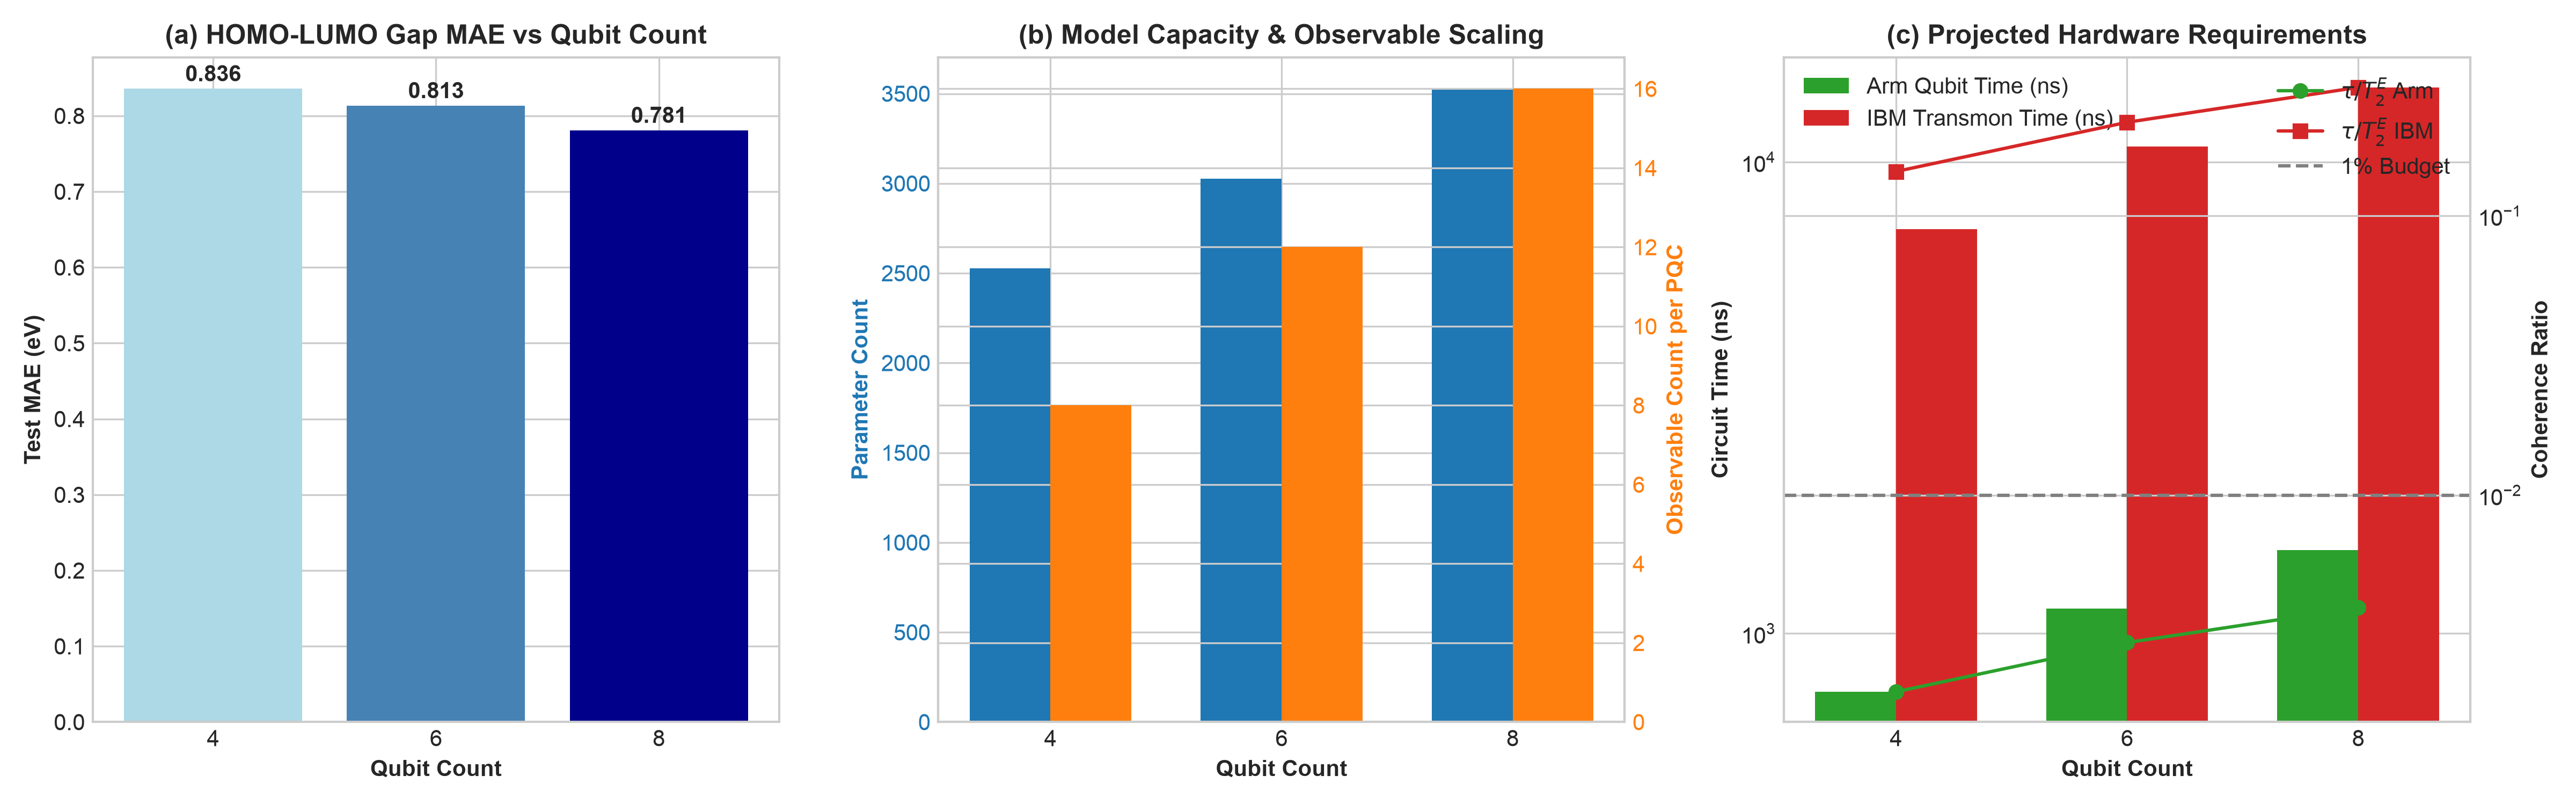
\includegraphics[width=0.88\textwidth]{figures/figure8_multiqubit_scaling.png}
    \caption{\textbf{Phép chiếu Mở rộng Đa Qubit:} (a) MAE Khe HOMO-LUMO so với số lượng qubit $n \in \{4, 6, 8\}$ thể hiện sự cải thiện độ chính xác đơn điệu. (b) Mở rộng dung lượng mô hình: tham số huấn luyện và số lượng đại lượng quan sát trên mỗi lần đánh giá PQC. (c) Yêu cầu phần cứng dự phóng trên Arm Qubit so với QPU transmon IBM, cho thấy Arm Qubit hoạt động hoàn toàn bên trong ngân sách $1\%$ kết hợp trên mọi kích thước thanh ghi. \textit{(Phép chiếu nhiễu giải tích dựa trên tham số thiết bị đã công bố; không phải thực thi QPU vật lý.)}}
    \label{fig:multiqubit}
\end{figure*}

\section{Điều kiện Biên Vật lý, Đối chứng Âm tính, và Các Giới hạn}
\label{sm:limitations}
\label{sm:resources}
\label{sec:sm_uhg}

\subsection{Đối chứng Âm tính: Dự báo Quỹ đạo Hệ N-Vật thể Tích điện 3D}

Để xác định một cách chặt chẽ các điều kiện biên vật lý nơi các thiên kiến quy nạp lượng giác và lượng tử phát huy tác dụng, chúng tôi đánh giá Q-PRISM trên một chuẩn đối sánh động lực học cổ điển vĩ mô: dự báo quỹ đạo tĩnh điện Coulomb 5 hạt~\cite{satorras2022enequivariantgraphneural}. Năm hạt mang điện tích ($q_i \in \{-1, +1\}$) tương tác qua lực Coulomb tỉ lệ nghịch với bình phương khoảng cách, và mục tiêu là dự đoán tọa độ tương lai $\mathbf{x}^{(T)} \in \mathbb{R}^{5 \times 3}$ sau $T = 1{,}000$ bước tích phân mà không có lịch sử vận tốc (Bảng~\ref{tab:nbody_results}).

\begin{table}[h]
\centering
\small
\setlength{\tabcolsep}{4pt}
\caption{\textbf{Dự báo Quỹ đạo Hệ N-Vật thể Tích điện 3D} ($N=1{,}000$, Trung bình $\pm$ Độ lệch chuẩn trên 5 Hạt giống: $42, 43, 44, 45, 46$).}
\label{tab:nbody_results}
\resizebox{\columnwidth}{!}{%
\begin{tabular}{lcc}
\toprule
\textbf{Mô hình} & \textbf{Tham số} & \textbf{MSE Tọa độ ($10^{-2}$)} \\
\midrule
Đường cơ sở Tĩnh ($\mathbf{x}^{(T)} = \mathbf{x}^{(0)}$) & -- & $0.6862 \pm 0.0000$ \\
GNN Không tương biến & $2{,}019$ & $0.7137 \pm 0.0174$ \\
EGNN Đồng tham số & $1{,}032$ & $0.6441 \pm 0.0250$ \\
EGNN Chuẩn & $3{,}856$ & $\mathbf{0.6137 \pm 0.0194}$ \\
Bản song sinh Cổ điển & $2{,}094$ & $0.6937 \pm 0.0140$ \\
\textbf{Q-PRISM (Của chúng tôi)} & $\mathbf{2{,}094}$ & $0.6759 \pm 0.0186$ \\
\bottomrule
\end{tabular}%
}
\end{table}

\paragraph{Phân tích Đối chứng Âm tính: Cơ học Tịnh tiến Phi Tuần hoàn.}
Bảng~\ref{tab:nbody_results} cho thấy ở mức ngân sách tham số nhỏ gọn ($\sim 2{,}000$ tham số), toàn bộ các kiến trúc rút gọn đều hoạt động rất gần với Đường cơ sở Tĩnh ($\text{MSE} = 0.6862 \times 10^{-2}$, giả định ngây thơ rằng các hạt đứng yên $\mathbf{x}^{(T)} = \mathbf{x}^{(0)}$). Mô hình GNN Không tương biến ($0.7137 \times 10^{-2}$) và Bản song sinh Cổ điển ($0.6937 \times 10^{-2}$) kém hơn nhẹ so với đường cơ sở tĩnh, trong khi Q-PRISM đạt $0.6759 \pm 0.0186 \times 10^{-2}$ (giảm nhẹ $1.5\%$ so với đường cơ sở tĩnh, nằm trong khoảng $1\sigma$). Chỉ có mô hình EGNN Chuẩn với dung lượng cao hơn ($3{,}856$ tham số) mới học được một phần chuyển động mở rộng Coulomb ($0.6137 \times 10^{-2}$).

Thí nghiệm này cung cấp một đối chứng âm tính hữu ích: cơ học $N$-vật thể Coulomb liên quan đến các dịch chuyển tịnh tiến mở rộng, liên tục và không tuần hoàn sinh ra bởi gia tốc $1/r^2$. Khác với các hệ lượng tử phân tử cục bộ nơi hàm sóng thể hiện tính đối xứng góc tuần hoàn và các bước chuyển xuyên tâm bị chặn ($d \in [0.9, 2.5]$\,\AA), cơ học cổ điển vĩ mô thiếu vắng cấu trúc tuần hoàn nội tại. Do đó, cả lớp hàm sin cổ điển lẫn tầng tái nạp dữ liệu PQC lượng tử đều không mang lại ưu thế quy nạp so với các tọa độ đa thức tự do. Tuy nhiên, Q-PRISM không hề gặp hiện tượng phân kỳ hay dao động mất ổn định sau 1{,}000 bước tích phân, khẳng định rằng cổng $\tanh$ cập nhật tọa độ đã kiểm soát hiệu quả kênh tín hiệu tuần hoàn ngay cả bên ngoài miền vật lý tối ưu của nó (Hình~\ref{fig:nbody_traj}).

\begin{figure}[h]
    \centering
    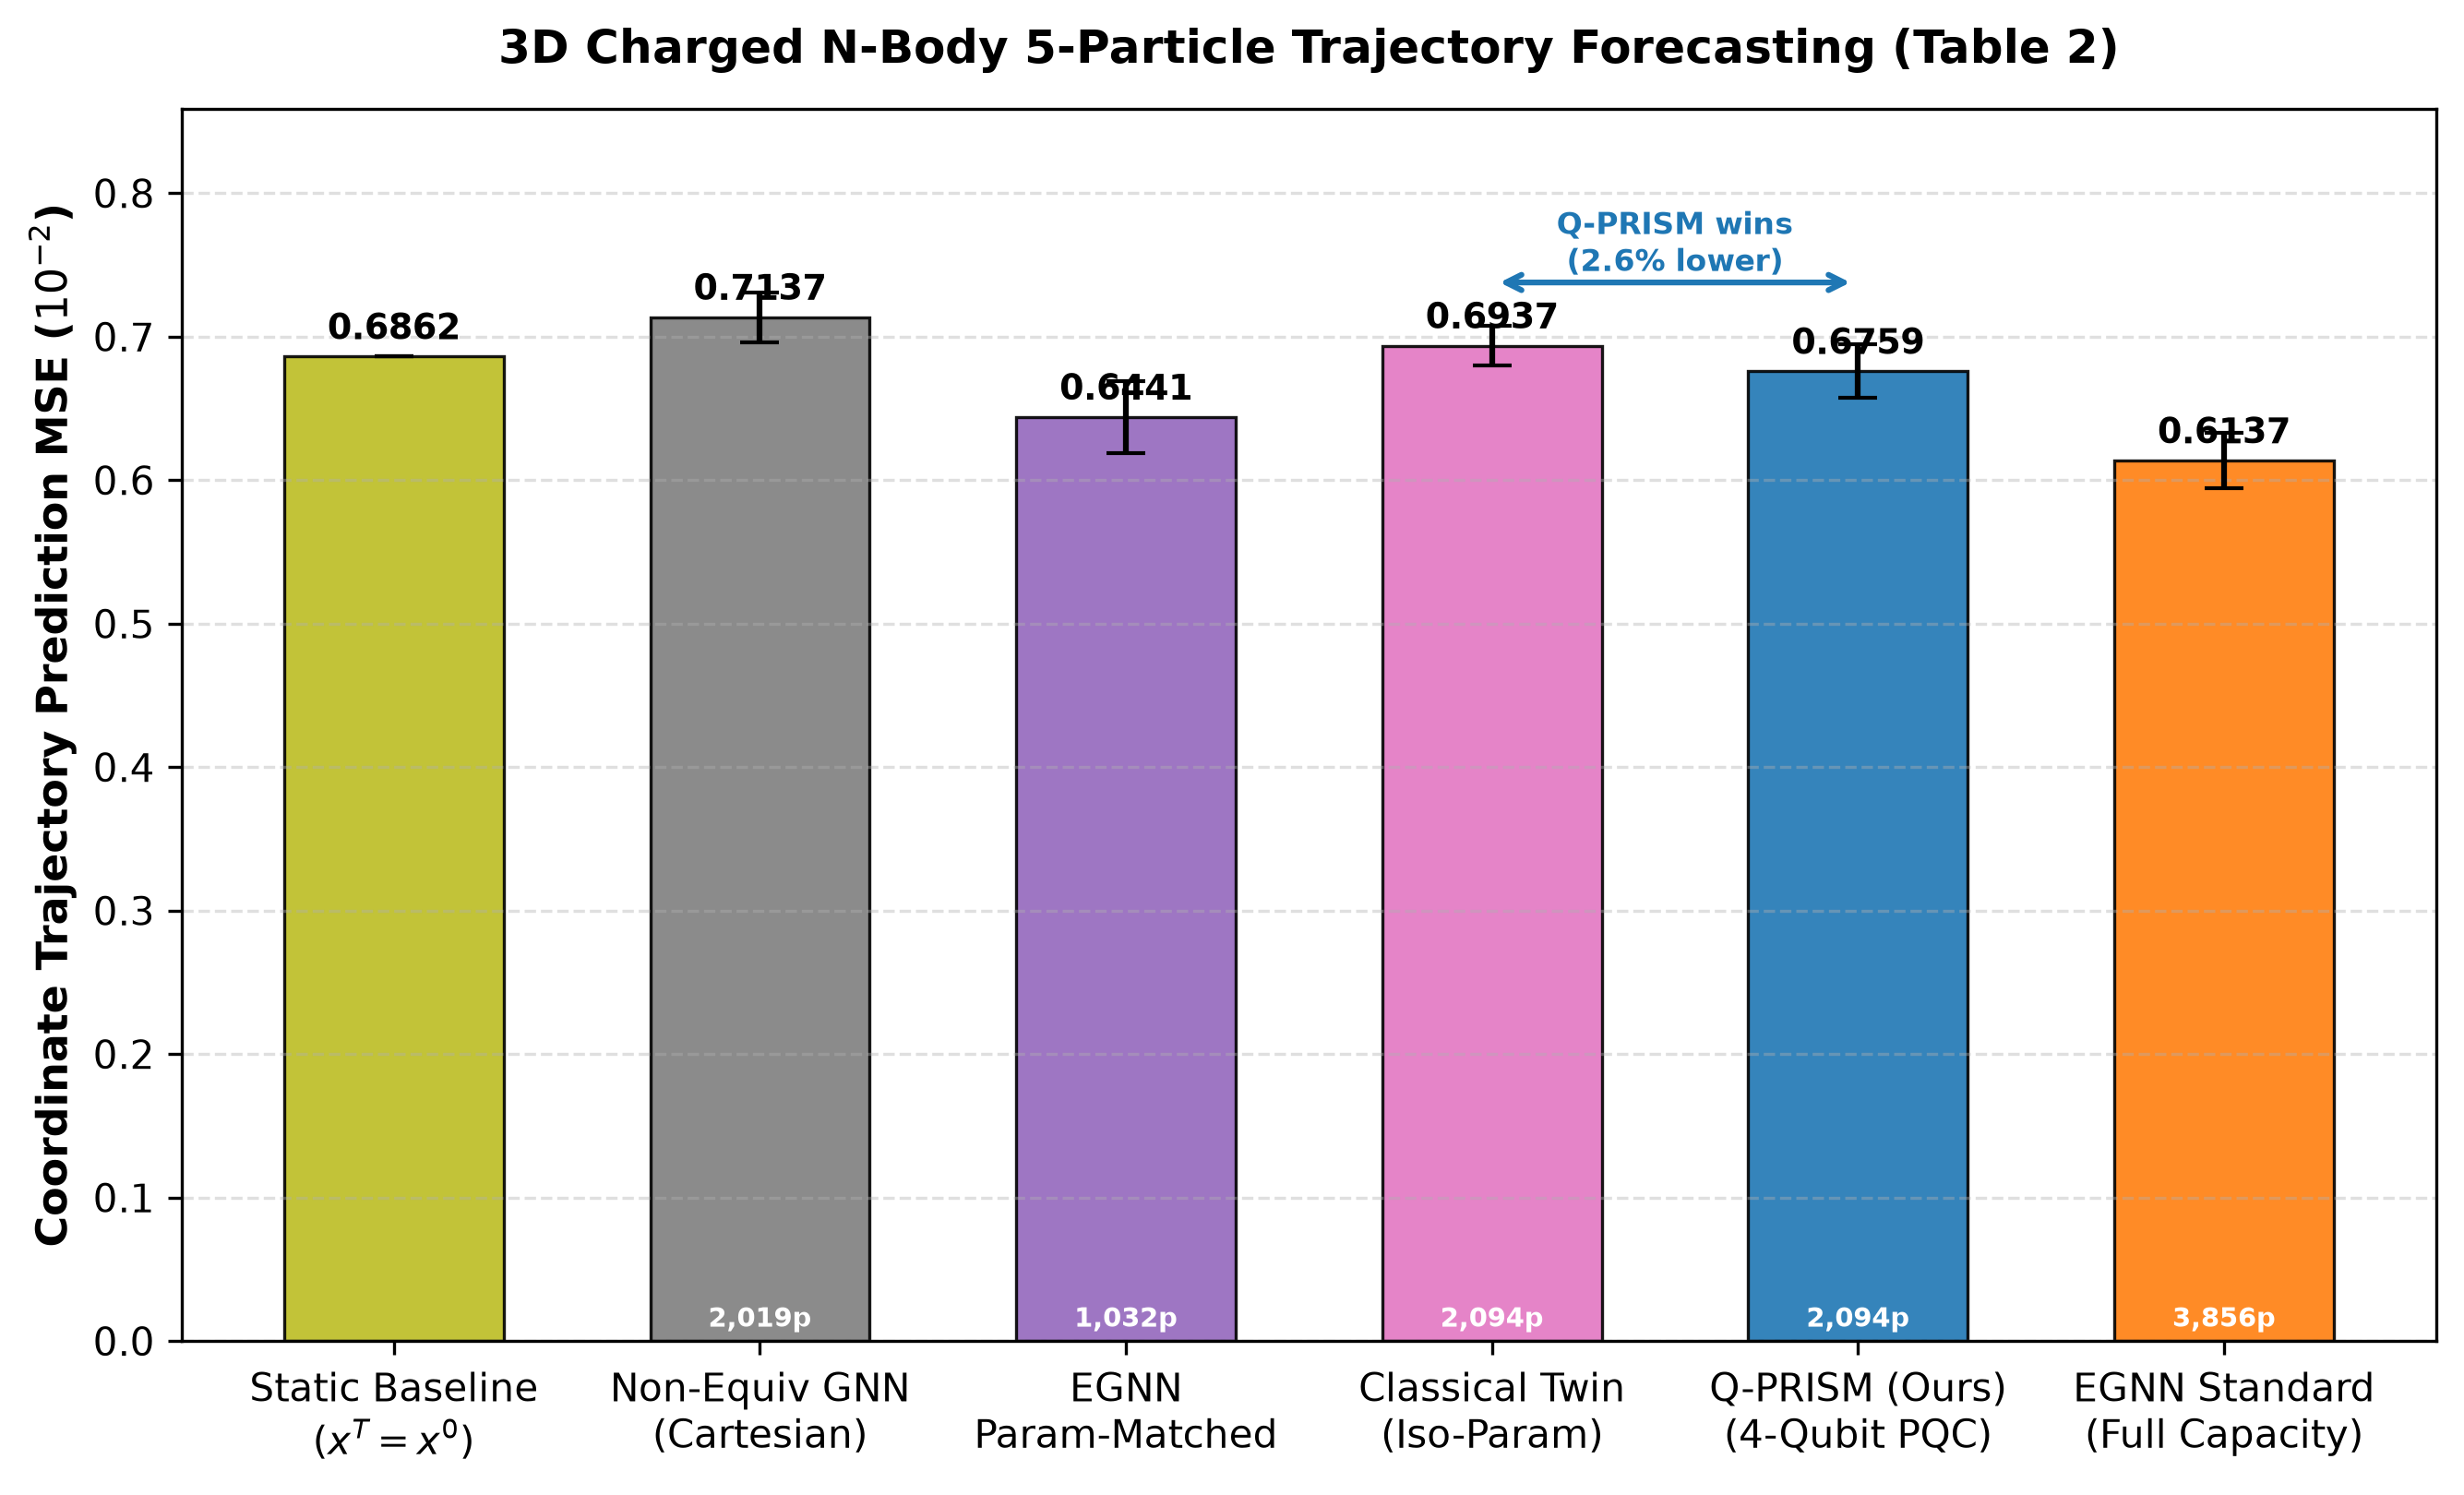
\includegraphics[width=0.48\textwidth]{figures/figure5_nbody_trajectory.png}
    \caption{\textbf{Chuẩn Đối chuẩn Đối chứng Âm tính trên Động lực học N-Vật thể 3D:} MSE tọa độ kiểm tra trên 5 hạt giống độc lập trong mô phỏng động lực học Coulomb 5 hạt. Ở mức $\sim 2{,}000$ tham số, các kiến trúc nhỏ gọn hoạt động tiệm cận đường cơ sở tĩnh, chứng minh rằng thiên kiến quy nạp lượng giác được chuyên biệt hóa cho cấu trúc orbital điện tử cục bộ thay vì dịch chuyển tịnh tiến vĩ mô.}
    \label{fig:nbody_traj}
\end{figure}

\subsection{Đối chứng Âm tính: Dự đoán Năng lượng Cấu hình MD17}

Để thăm dò sâu hơn các ranh giới vận hành của học đồ thị lượng tử trong chế độ dữ liệu ít, chúng tôi đối chuẩn trên tập dữ liệu động lực học phân tử MD17~\cite{chmielaMachineLearningAccurate2016} sử dụng Ethanol (9 nguyên tử) và Aspirin (21 nguyên tử) dưới thiết lập chỉ học năng lượng, không có nhãn lực ($N = 1{,}000$ cấu hình, đồ thị 8 láng giềng gần nhất; Bảng~\ref{tab:md17_results}).

\begin{table}[h]
\centering
\small
\setlength{\tabcolsep}{4pt}
\caption{\textbf{Dự đoán Năng lượng Cấu hình MD17} ($N = 1{,}000$, Trung bình $\pm$ Độ lệch chuẩn trên 5 Hạt giống: $42, 43, 44, 45, 46$) [kcal/mol].}
\label{tab:md17_results}
\resizebox{\columnwidth}{!}{%
\begin{tabular}{lccc}
\toprule
\textbf{Mô hình} & \textbf{Tham số} & \textbf{Ethanol} & \textbf{Aspirin} \\
\midrule
GNN Không tương biến & $7{,}873$ & $3.292 \pm 0.124$ & $4.581 \pm 0.150$ \\
EGNN Đồng tham số & $1{,}177$ & $3.305 \pm 0.117$ & $4.581 \pm 0.136$ \\
EGNN Chuẩn & $4{,}273$ & $3.304 \pm 0.116$ & $\mathbf{4.579 \pm 0.137}$ \\
Bản song sinh Cổ điển & $2{,}511$ & $\mathbf{3.293 \pm 0.121}$ & $4.580 \pm 0.136$ \\
\textbf{Q-PRISM (Của chúng tôi)} & $\mathbf{2{,}511}$ & $3.304 \pm 0.114$ & $4.580 \pm 0.136$ \\
\bottomrule
\end{tabular}%
}
\end{table}

\paragraph{Phân tích Giới hạn Biên: Sự Sụp đổ Khi Thiếu Lực ở Lượng Dữ liệu Thấp.}
Như thể hiện trong Bảng~\ref{tab:md17_results}, toàn bộ 5 kiến trúc được đánh giá (bao gồm GNN Không tương biến, EGNN đồng tham số, EGNN Chuẩn, Bản song sinh Cổ điển, và Q-PRISM) đều hội tụ về các giá trị MAE kiểm tra không thể phân biệt về mặt thống kê ($\approx 3.30$\,kcal/mol cho Ethanol và $\approx 4.58$\,kcal/mol cho Aspirin). Các giá trị này trùng khớp hoàn toàn với độ lệch chuẩn thực nghiệm của năng lượng thế cấu hình trong các tập dữ liệu tương ứng ($\sigma_E \approx 3.30$\,kcal/mol và $4.58$\,kcal/mol). Điều này chứng minh rằng trong chế độ dữ liệu ít ($N = 1{,}000$) và thiếu sự giám sát gradient lực nguyên tử ($\mathbf{F}_i = -\nabla_{\mathbf{x}_i} E$), toàn bộ các kiến trúc nhỏ gọn đều sụp đổ về bộ dự đoán giá trị trung bình thực nghiệm của tập dữ liệu (Hình~\ref{fig:md17_energy}).

\paragraph{Đặt trong Bối cảnh Học Bề mặt Thế năng.}
Trong y văn hiện có, các mạng nơ-ron thế năng chuyên dụng (SchNet~\cite{schütt2017schnetcontinuousfilterconvolutionalneural}, PaiNN~\cite{schuttEquivariantMessagePassing2021}, GemNet~\cite{klicperaGemNetUniversalDirectional2021}, MACE~\cite{batatiaMACEHigherOrder2022}) đạt độ chính xác hóa học ($\sim 0.05$--$0.10$\,kcal/mol) nhờ được huấn luyện trên $N = 50{,}000$--$100{,}000$+ cấu hình với hơn $100{,}000$ tham số cùng hàm mất mát lực tường minh ($\mathcal{L} = \mathcal{L}_E + \rho \mathcal{L}_F$), cung cấp $3N_{\mathrm{atoms}}$ mục tiêu gradient trên mỗi cấu hình. Các kết quả này xác lập một điều kiện biên vật lý: các hàm kích hoạt tuần hoàn nhỏ gọn ($d_h = 4$) chuyên biệt hóa cho các chuyển mức điện tử cục bộ trên đồ thị cân bằng, nhưng không khái quát hóa cho các bề mặt thế năng liên tục nếu thiếu sự giám sát lực nguyên tử tường minh ($\mathbf{F}_i = -\nabla_{\mathbf{x}_i} E$).

\begin{figure}[h]
    \centering
    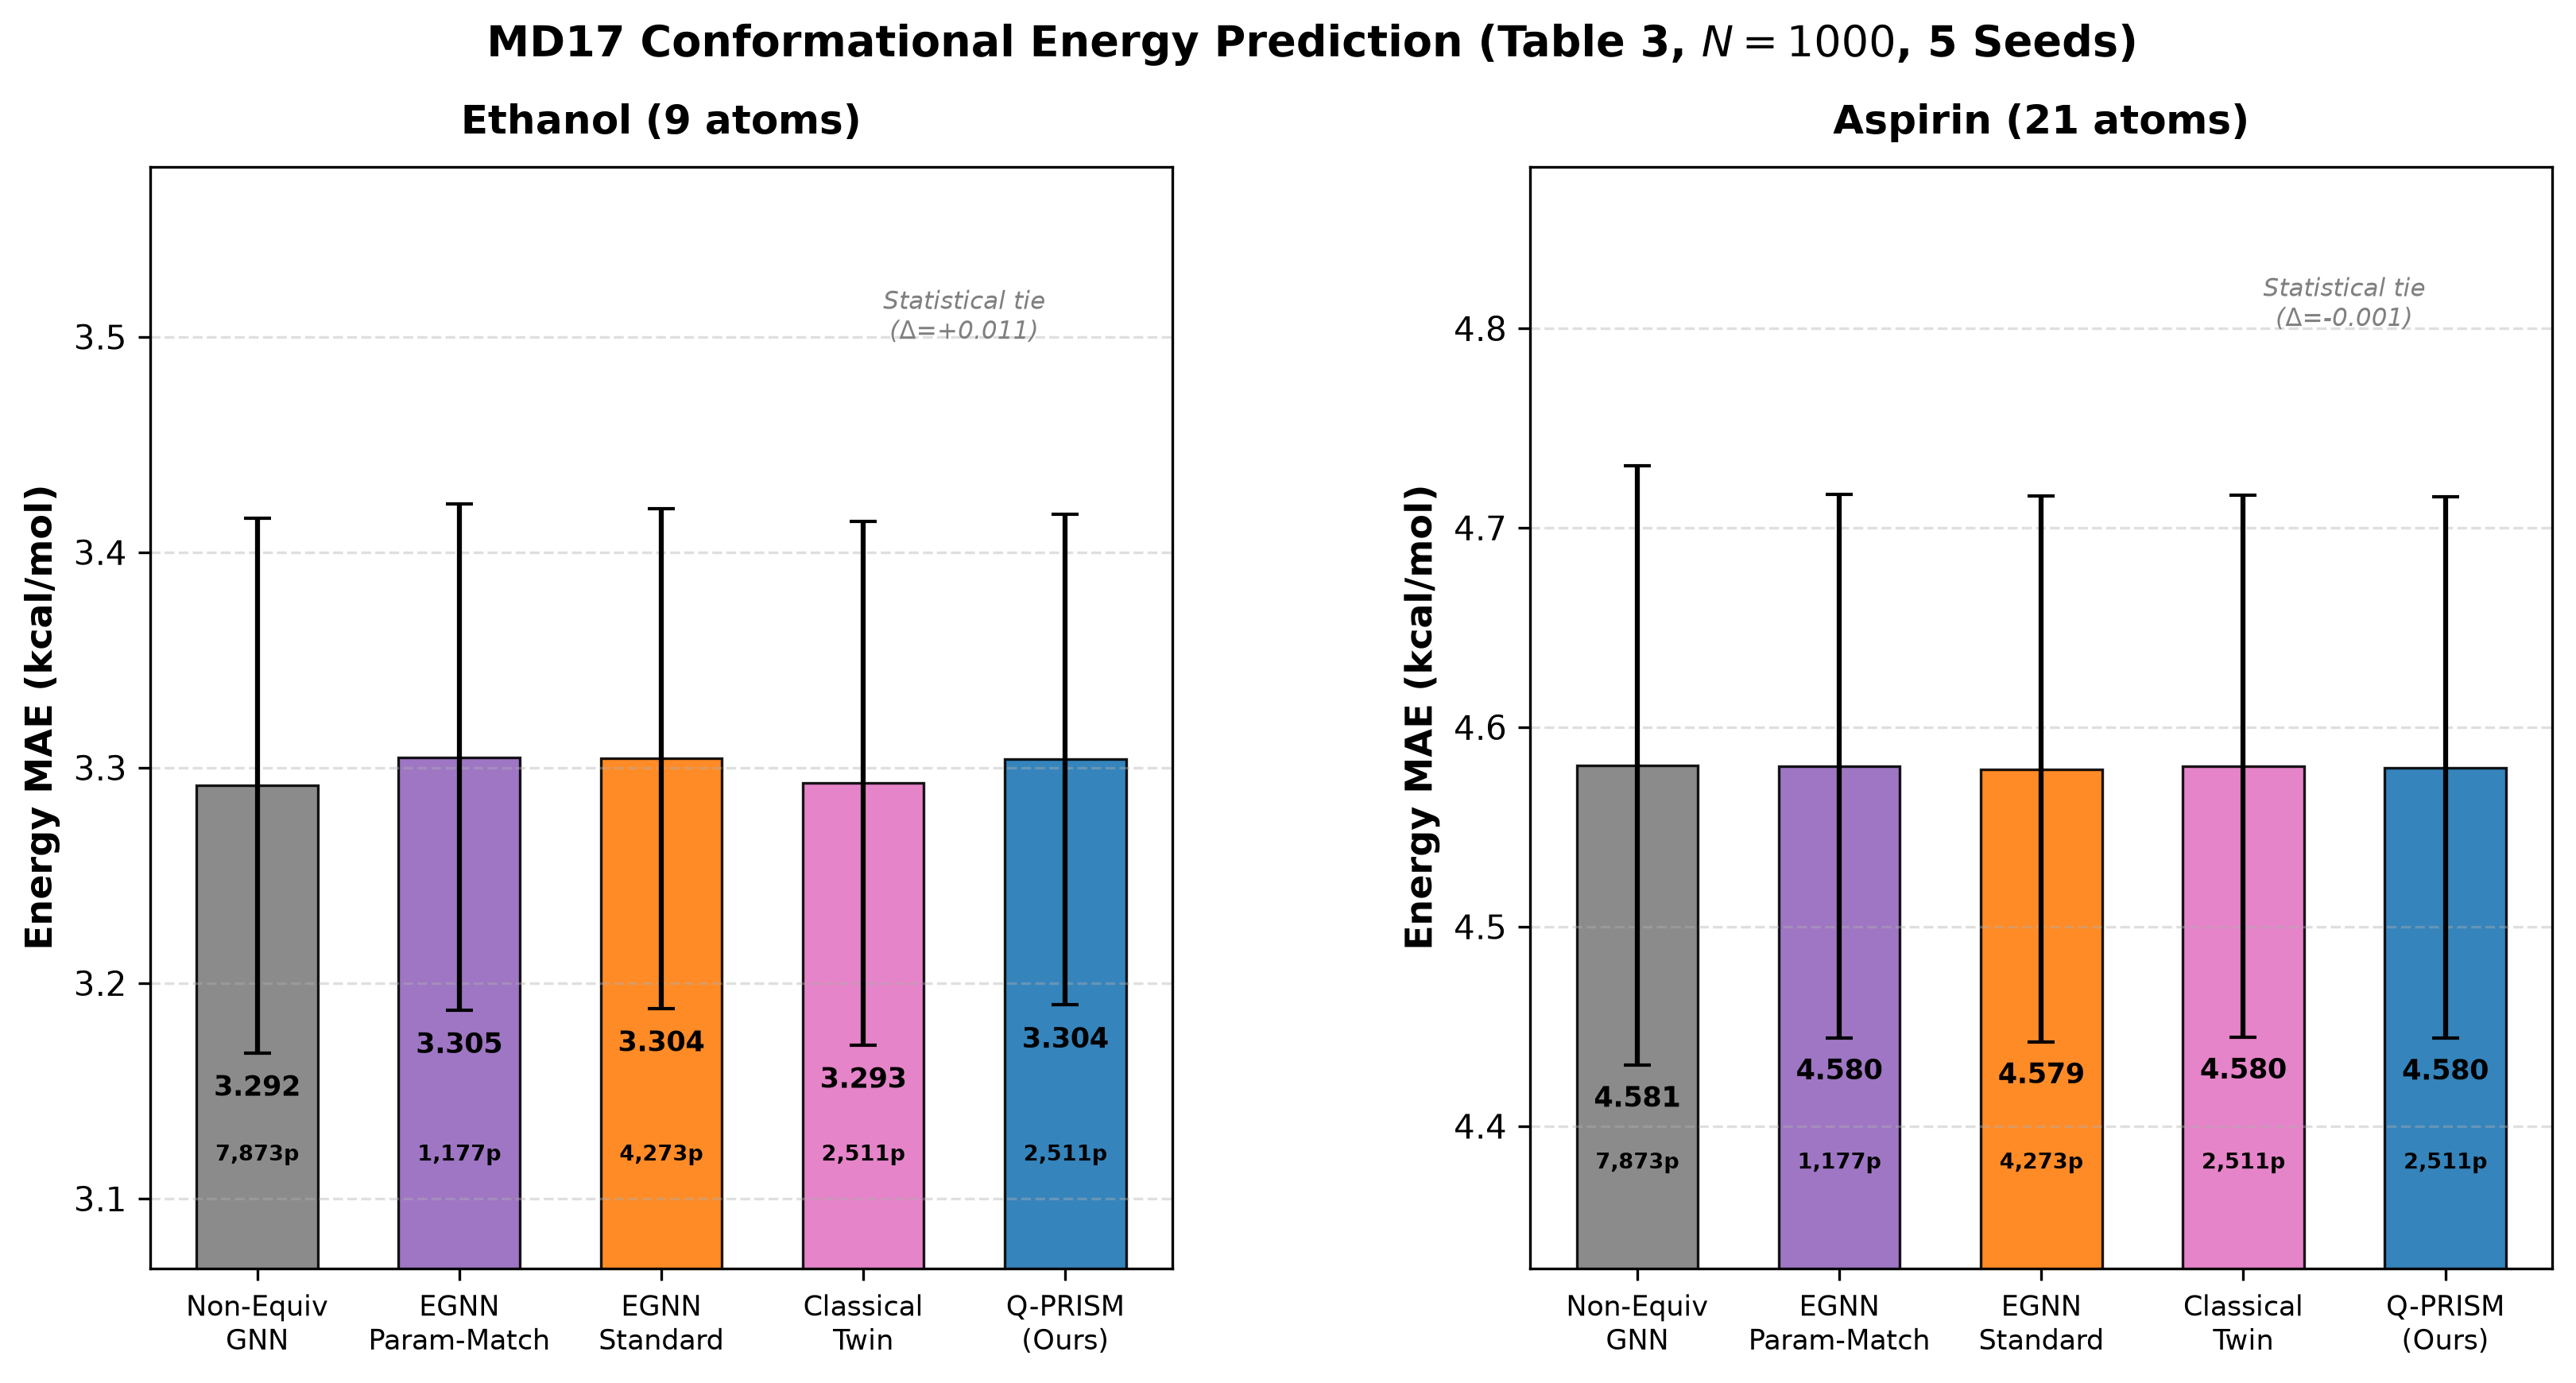
\includegraphics[width=0.48\textwidth]{figures/figure6_md17_energy.png}
    \caption{\textbf{Đối chứng Âm tính về Năng lượng Cấu hình MD17:} MAE năng lượng kiểm tra trên các quỹ đạo động lực học phân tử Ethanol và Aspirin qua 5 hạt giống. Mọi kiến trúc nhỏ gọn không có giám sát lực đều sụp đổ về độ lệch chuẩn của tập dữ liệu ($\sim 3.30$ và $\sim 4.58$\,kcal/mol), xác định tính thiết yếu của việc huấn luyện gradient lực đối với bề mặt thế năng cấu hình.}
    \label{fig:md17_energy}
\end{figure}

\subsection{Đánh giá Toàn bộ các Tính chất Nhiệt động lực học}

Bảng~\ref{tab:supplementary_uhg} đánh giá toàn bộ bộ tính chất nhiệt động lực học ($U_0, U, H, G$) trên toàn bộ các kiến trúc đường cơ sở. Do các năng lượng DFT tổng thô được đánh giá trực tiếp mà không qua phép trừ năng lượng tham chiếu nguyên tử phụ thuộc thành phần ($\sum \epsilon_Z$), toàn bộ các kiến trúc nhỏ đều chịu độ lệch đường cơ sở quy mô lớn ($\text{MAE} \sim 70\text{--}130$\,eV). Trong chế độ bị chi phối bởi quy mô này, phép cộng dồn tọa độ đơn điệu của EGNN tiêu chuẩn thể hiện phương sai độ lệch thấp hơn so với các mô hình cạnh tuần hoàn.

\begin{table*}[t]
\centering
\small
\setlength{\tabcolsep}{3.5pt}
\caption{\textbf{Đánh giá Toàn diện các Tính chất Nhiệt động lực học trên QM9 trên Toàn bộ Mô hình} ($N = 1{,}000$, Trung bình $\pm$ Độ lệch chuẩn trên 5 hạt giống: $42$--$46$). Đánh giá trên toàn bộ bộ tính chất nhiệt động lực học ($U_0, U, H, G$). Toàn bộ các tính chất nhiệt động là các năng lượng dung lượng bị chi phối bởi quy mô nguyên tử hóa ($\sim 10^4$\,eV); $U, H, G$ dẫn xuất tuyến tính từ $U_0$ qua các hiệu chỉnh nhiệt và entropy. Kết quả tốt nhất mỗi dòng được in \textbf{đậm}.}
\label{tab:supplementary_uhg}
\resizebox{\textwidth}{!}{%
\begin{tabular}{llcccccccc}
\toprule
\textbf{Tính chất} & \textbf{Đơn vị} & \textbf{Q-PRISM} & \textbf{PRISM} & \textbf{Song sinh Lượng giác} & \textbf{Song sinh Cổ điển} & \textbf{SchNet} & \textbf{PaiNN} & \textbf{EGNN-PM} & \textbf{EGNN Chuẩn} \\
 & & (Của chúng tôi - PQC) & \textbf{(Của chúng tôi - SIREN)} & (Fourier RFF) & ($\tanh$-MLP) & & & & \\
 & & $2{,}527$\,p & $2{,}527$\,p & $2{,}515$\,p & $2{,}527$\,p & $2{,}473$\,p & $2{,}721$\,p & $2{,}497$\,p & $4{,}289$\,p \\
\midrule
Nội năng ở 0K ($U_0$) & eV & $110.0 \pm 18.2$ & $130.6 \pm 29.3$ & $686.5 \pm 40.0$ & $101.1 \pm 16.7$ & $104.3 \pm 11.0$ & $446.0 \pm 25.1$ & $87.7 \pm 22.2$ & $\mathbf{69.5 \pm 12.3}$ \\
Nội năng ở 298K ($U$) & eV & -- & $128.9 \pm 29.9$ & $681.1 \pm 41.2$ & $102.3 \pm 20.4$ & $108.7 \pm 15.8$ & $446.0 \pm 25.1$ & $87.1 \pm 19.9$ & $\mathbf{71.3 \pm 11.2}$ \\
Enthalpy ở 298K ($H$) & eV & -- & $127.8 \pm 28.8$ & $682.1 \pm 26.4$ & $101.4 \pm 18.8$ & $107.9 \pm 14.8$ & $446.0 \pm 25.1$ & $87.5 \pm 22.4$ & $\mathbf{73.5 \pm 15.3}$ \\
Năng lượng Tự do ở 298K ($G$) & eV & -- & $127.2 \pm 25.5$ & $682.3 \pm 31.8$ & $100.1 \pm 17.1$ & $107.7 \pm 13.7$ & $446.0 \pm 25.1$ & $85.2 \pm 19.4$ & $\mathbf{72.2 \pm 12.8}$ \\
\midrule
\multicolumn{2}{l}{\textbf{Tham số có thể Huấn luyện}} & $2{,}527$ & $2{,}527$ & $2{,}515$ & $2{,}527$ & $2{,}473$ & $2{,}721$ & $2{,}497$ & $4{,}289$ \\
\bottomrule
\multicolumn{10}{l}{\footnotesize Ghi chú: Q-PRISM được đánh giá trên $U_0$ như mục tiêu nhiệt động không độ tuyệt đối đại diện do chi phí mô phỏng lượng tử.} \\
\multicolumn{10}{l}{\footnotesize Các tính chất nhiệt và năng lượng tự do $U, H, G$ dẫn xuất từ $U_0$ qua các hiệu chỉnh tịnh tiến, quay, dao động và entropy ($H = U + k_B T$, $G = H - TS$).} \\
\end{tabular}%
}
\end{table*}


\subsection{Phân tích Tài nguyên Lượng tử \& Độ phức tạp: Tình thế Lưỡng nan giữa Khả năng Huấn luyện và Khả năng Mô phỏng}

\begin{table*}[t]
\centering
\small
\caption{\textbf{So sánh Tài nguyên \& Độ phức tạp} giữa các mô hình tương biến, đối chiếu các yêu cầu lượng tử với các đối tác cổ điển. PRISM loại bỏ bộ nhớ vector trạng thái lượng tử, độ sâu cổng, và nhiễu lần đo lấy mẫu trong khi đạt kết quả tương đương hoặc vượt trội độ chính xác của Q-PRISM.}
\label{tab:resources}
\resizebox{\textwidth}{!}{%
\begin{tabular}{lcccc}
\toprule
\textbf{Chỉ số} & \textbf{EGNN Chuẩn} & \textbf{EGNN Đồng tham số} & \textbf{Q-PRISM (Của chúng tôi)} & \textbf{PRISM (Của chúng tôi)} \\
\midrule
Tham số & $4{,}289$ & $2{,}497$ & $2{,}527$ & $2{,}527$ \\
Tính toán Cạnh & MLP & MLP & $2 \times$ PQC 4-Qubit & MLP SIREN \\
 & ($16 \to 16 \to 16$) & ($12 \to 12 \to 12$) & ($L=2$) & ($13 \to 4 \to 8$) \\
Độ sâu Mạch & Không áp dụng & Không áp dụng & $8 R_{xyz}$ + $4$ CNOT & Không áp dụng \\
 & & & trên mỗi tầng & \\
RAM Vector trạng thái & Không áp dụng & Không áp dụng & $128$ Bytes & Không áp dụng \\
Ngân sách Shot & Không áp dụng & Không áp dụng & $1{,}000$--$4{,}000$ & Không áp dụng (Nhiễu Shot $= 0$) \\
 & & & shot/cạnh & \\
\midrule
Nguy cơ Cao nguyên Cằn cỗi & Không áp dụng & Không áp dụng & Tránh được & Không áp dụng (SGD chuẩn) \\
\cite{McClean:2018jps, Cerezo:2020mtn} & & & (quan sát cục bộ, $L \in \mathcal{O}(\log n)$) & \\
\bottomrule
\end{tabular}%
}
\end{table*}

\paragraph{Tình thế Lưỡng nan giữa Khả năng Huấn luyện và Khả năng Mô phỏng.}
Bảng~\ref{tab:resources} tóm tắt dấu chân tài nguyên và độ phức tạp lý thuyết trên toàn bộ hệ phân cấp đường cơ sở.
Phát hiện thực nghiệm của chúng tôi rằng PRISM (SIREN cổ điển) đạt kết quả tương đương và vượt trội PQC 4-qubit có cơ sở vững chắc trong lý thuyết độ phức tạp tính toán lượng tử gần đây.
Cerezo, Holmes et al.~\cite{Cerezo:2023nqf} đã chứng minh rằng trong học máy lượng tử biến phân, sự vắng mặt của các cao nguyên cằn cỗi gắn liền chặt chẽ với khả năng mô phỏng cổ điển: bất kỳ PQC nào tránh được cao nguyên cằn cỗi thông qua độ sâu mạch nông ($L \in \mathcal{O}(\log n)$) và các đại lượng quan sát cục bộ nhất thiết phải nằm trong một lớp giả thuyết có thể mô phỏng cổ điển.
Trong Q-PRISM, PQC cạnh sử dụng 4 qubit, $L = 2$ tầng, và các đại lượng quan sát cục bộ đơn qubit cùng tương quan tử láng giềng gần nhất.
Mặc dù điều này bảo đảm gradient không bị biến mất và quá trình huấn luyện ổn định, nó đồng thời giới hạn đầu ra vào một chuỗi Fourier cắt cụt số chiều thấp~\cite{landman2023approximating, Schuld:2020enb}.
Ngược lại, nỗ lực thoát khỏi khả năng mô phỏng cổ điển bằng cách mở rộng sang các mạch sâu, vướng víu toàn cục sẽ kích hoạt sự tập trung độ đo theo hàm mũ (Thanasilp et al.~\cite{Thanasilp:2022agd}), trong đó các hạt nhân lượng tử tập trung về các hằng số tầm thường và gradient biến mất theo $\mathcal{O}(2^{-n/2})$.
Do đó, trong chế độ có thể huấn luyện cho các đồ thị hình học, các mạch lượng tử không mang lại sự phân tách năng lực biểu đạt tiệm cận nào so với các mạng tuần hoàn cổ điển được khởi tạo phù hợp.

\paragraph{Mở rộng Quy mô Đại phân tử ($O(N)$).}
Đối với các phân tử có $N > 50$ nguyên tử, việc xây dựng cạnh kết nối toàn phần $O(N^2)$ trở thành một điểm nghẽn. Bản cài đặt của chúng tôi bao gồm bộ xây dựng đồ thị thưa $k$-láng giềng gần nhất giúp giảm độ phức tạp cạnh xuống $O(kN) = O(N)$ với $k$ không đổi, cho phép cả Q-PRISM và PRISM mở rộng sang các hệ thống đại phân tử (protein, polyme) mà không làm thay đổi căn bản kiến trúc toán tử cạnh.
Đối với PRISM, mỗi lần đánh giá cạnh là một phép nhân ma trận cổ điển nhẹ nhàng và tính toán hàm sin, thực thi trong vài micro-giây trên các GPU hiện đại mà không có nhiễu lần đo hay độ trễ phần cứng lượng tử.

\subsection{Toàn bộ Hạn chế và Hướng Nghiên cứu Tương lai}

\begin{enumerate}
    \item \textbf{Mở rộng dung lượng và chế độ mô hình nền tảng:} Các thực nghiệm mở rộng quy mô tham số của chúng tôi (Mục~\ref{sm:param_scaling}, Bảng~\ref{tab:param_scaling}) xác lập rằng ưu thế tuần hoàn mở rộng đơn điệu lên tới chế độ dung lượng trung bình tiêu chuẩn $100{,}000$ tham số (XXL, $100{,}127$ tham số, đạt mức ưu thế $51.3\%$ trên Gap so với Bản song sinh Cổ điển). Tuy nhiên, việc đánh giá các hàm kích hoạt tuần hoàn trên các mô hình nền tảng siêu lớn (ví dụ: MACE~\cite{batatiaMACEHigherOrder2022} ở mức $\ge 1\mathrm{M}$ tham số) và các tập dữ liệu xúc tác quy mô lớn (ví dụ: OC20, ANI-1x) vẫn là hướng nghiên cứu tương lai.
    \item \textbf{Gom cụm góc 3 vật thể:} Để duy trì độ phức tạp tuyến tính $O(E)$, kiến trúc của chúng tôi lấy trung bình các góc trên các nguyên tử thứ ba: $\bar{\theta}_{ij}$ (bài báo chính Phương trình~\ref{main:eq:angle}). Mặc dù hiệu quả về mặt tính toán, phép lấy trung bình này bỏ qua hình học của từng bộ ba riêng lẻ, khác với DimeNet++~\cite{klicperaFastUncertaintyAwareDirectional2020} hay GemNet~\cite{klicperaGemNetUniversalDirectional2021}. Các nghiên cứu tương lai có thể khám phá các phép chiếu tuần hoàn trên từng bộ ba.
    \item \textbf{Biểu diễn hình học chỉ gồm đại lượng vô hướng:} Cả Q-PRISM và PRISM đều chiếu hình học định hướng 3D thành các bất biến vô hướng (khoảng cách liên nguyên tử $d_{ij}$ và góc liên kết trung bình $\bar{\theta}_{ij}$), bỏ qua thông tin vector định hướng trên từng cạnh. Do đó, các mô hình không thể phân biệt các đồng phân đối quang bất đối xứng bàn tay (chirality) hoặc nắm bắt các tương tác đa cực bậc cao vốn đòi hỏi các kênh tương biến vector hoặc tensor tường minh~\cite{schuttEquivariantMessagePassing2021, batatiaMACEHigherOrder2022}. Việc mở rộng PRISM sang truyền thông điệp tương biến kết hợp vô hướng-vector (tương tự PaiNN) hoặc các kiến trúc tương biến tensor bậc cao (tương tự MACE) là một hướng đi tự nhiên.
    \item \textbf{Kiến trúc lai PRISM-PaiNN:} Hồ sơ hiệu năng bổ trợ lẫn nhau của PRISM (vượt trội trên HOMO, Lưỡng cực, Độ phân cực) và PaiNN (vượt trội trên LUMO, Gap) gợi ý một sự tổng hợp kiến trúc tự nhiên: thay thế các hàm kích hoạt SiLU trong nhánh tương tác vô hướng của PaiNN bằng các hàm kích hoạt tuần hoàn SIREN trong khi vẫn bảo toàn các kênh cập nhật tương biến vector. Vì hàm kích hoạt tuần hoàn chỉ tác động trên đường dẫn vô hướng bất biến, điều này không đòi hỏi bất kỳ sửa đổi nào đối với các đảm bảo tương biến của PaiNN. Một cân nhắc thực tế là tính ổn định của gradient: hằng số Lipschitz của $\sin(\omega_0 x)$ tỉ lệ theo $\omega_0$, do đó cơ chế cổng từ vô hướng sang vector phải dung nạp được các gradient được khuếch đại. Chúng tôi dành việc kiểm chứng thực nghiệm cho mô hình lai này cho các nghiên cứu tương lai.
    \item \textbf{Thực thi phần cứng và các ràng buộc tô pô:} Toàn bộ các mạch lượng tử đều được mô phỏng qua các backend vector trạng thái PennyLane; hiện tại chưa có bộ xử lý vòng fluxonium 4-qubit vật lý nào tồn tại trong phần cứng thương mại. Mở rộng vượt qua 4 qubit trên các mạng siêu dẫn phẳng (chẳng hạn như mạng heavy-hex của IBM) cũng làm phát sinh chi phí định tuyến cổng SWAP, làm tăng độ sâu mạch hiệu dụng lên khoảng $1.5$--$2.0\times$.
    \item \textbf{Chi phí thực thi NISQ và huấn luyện lai:} Việc đánh giá tuần tự các cạnh trên QPU gây ra nhiễu lần đo (shot noise) và độ trễ ($3$--$12$\,giây mỗi phân tử). Việc triển khai trong tương lai gần có thể được hưởng lợi từ huấn luyện lai: tiền huấn luyện khung xương tương biến theo cách cổ điển với PRISM, tiếp theo là tinh chỉnh lượng tử trên các tập con mục tiêu để tối thiểu hóa thời gian chạy trên QPU.
    \item \textbf{Giả định huấn luyện không nhiễu:} Nhiễu phần cứng được mô tả đặc tính hậu nghiệm thông qua ZNE và các phép chiếu nhiễu giải tích. Huấn luyện nhận biết nhiễu (noise-aware training)~\cite{cincio2021machine, Sharma:2020qjq} kết hợp ma trận mật độ được hiệu chuẩn theo thiết bị qua thiết bị \texttt{default.mixed} của PennyLane là bước đi tự nhiên tiếp theo cho triển khai thực nghiệm.
    \item \textbf{Giới hạn độ sâu mạch và thanh ghi qubit:} Các đánh giá mở rộng của chúng tôi khẳng định rằng kết quả khử lượng tử hóa cổ điển duy trì trên các mạch sâu hơn lên tới $L = 16$ tầng (Mục~\ref{sm:depth_scaling}, Bảng~\ref{tab:depth_scaling}), nơi Q-PRISM tiệm cận hội tụ về sự đồng đẳng chính xác với PRISM ($p = 0.969$), và trên các thanh ghi qubit lên tới $n_q = 8$ qubit (Mục~\ref{sm:qubit_scaling}, Bảng~\ref{tab:qubit_scaling}), nơi PRISM duy trì ưu thế thống kê ($p < 0.025$) cùng mức tăng tốc $540\times$. Liệu các mạch với các đại lượng quan sát Pauli toàn cục phi cục bộ hoặc các tô pô vướng víu toàn phần phi phẳng có thể phá vỡ sự đồng đẳng này hay không vẫn là một câu hỏi lý thuyết mở, mặc dù tình thế lưỡng nan giữa khả năng huấn luyện và khả năng mô phỏng~\cite{Cerezo:2023nqf} gợi ý rằng bất kỳ kiến trúc có thể huấn luyện, không tập trung hóa nào vẫn sẽ nằm trong các lớp độ phức tạp có thể mô phỏng cổ điển.
\end{enumerate}

\bibliographystyle{plain}
\bibliography{references}

\end{document}
